\documentclass[11pt,twoside,twocolumn]{usgsreport}
\usepackage{usgsfonts}
\usepackage{usgsgeo}
\usepackage{usgsidx}
\usepackage[figuretoc,tabletoc]{usgsreporta}

\usepackage{amsmath}
\usepackage{algorithm}
\usepackage{algpseudocode}
\usepackage{bm}
\usepackage{calc}
\usepackage{natbib}
\usepackage{graphicx}
\usepackage{longtable}

%Do not allow a page break to result in a line appearing by itself 
% https://tex.stackexchange.com/questions/4152/how-do-i-prevent-widow-orphan-lines 
\usepackage[all]{nowidow}

\makeindex
\usepackage{setspace}
% uncomment to make double space 
%\doublespacing
\usepackage{etoolbox}
\usepackage{verbatim}

% set up the listings package for highlighting block definitions and input files
\usepackage{listings}
\usepackage{xcolor}
\lstset{
  basicstyle=\footnotesize\ttfamily\color{black},
  numbers=none,
  columns=flexible,
  backgroundcolor=\color{yellow!10},
%  frame=tlbr,
  moredelim=**[is][\color{red}]{@}{@},
}
\lstdefinestyle{blockdefinition}{
  moredelim=**[is][\color{blue}]{@}{@},
}
%usage: \lstinputlisting[style=blockdefinition]{./mf6ivar/tex/gwf-chd-dimensions.dat}
\lstdefinestyle{inputfile}{
  morecomment=[l]\#,
  backgroundcolor=\color{gray!10},
}
%usage: \lstinputlisting[style=inputstyle]{file.dat}

\usepackage[hidelinks]{hyperref}
\hypersetup{
    pdftitle={MODFLOW 6 -- Description of Input and Output},
    pdfauthor={MODFLOW 6 Development Team},
    pdfsubject={numerical simulation groundwater flow},
    pdfkeywords={groundwater, MODFLOW, simulation},
    pdflang={en-US},
    bookmarksnumbered=true,     
    bookmarksopen=true,         
    bookmarksopenlevel=1,       
    colorlinks=true,
    allcolors={blue},          
    pdfstartview=Fit,           
    pdfpagemode=UseOutlines,
    pdfpagelayout=TwoPageRight
}

\graphicspath{{./Figures/}}
\newcommand{\modflowversion}{6.0.00}
\newcommand{\modflowdate}{August 10, 2017}
\newcommand{\currentmodflowversion}{Version \modflowversion---\modflowdate}


\newcommand{\mli}[1]{\mathit{#1}}

\renewcommand{\cooperator}
{the \textusgs\ Water Availability and Use Science Program}
\renewcommand{\reporttitle}
{MODFLOW 6 -- Description of Input and Output}
\renewcommand{\coverphoto}{coverimage.jpg}
\renewcommand{\GSphotocredit}{Binary computer code illustration.}
\renewcommand{\reportseries}{}
\renewcommand{\reportnumber}{}
\renewcommand{\reportyear}{2017}
\ifdef{\reportversion}{\renewcommand{\reportversion}{\currentmodflowversion}}{}
\renewcommand{\theauthors}{MODFLOW 6 Development Team}
\renewcommand{\thetitlepageauthors}{\theauthors}
%\renewcommand{\theauthorslastfirst}{}
\renewcommand{\reportcitingtheauthors}{\theauthors}
\renewcommand{\colophonmoreinfo}{}
\renewcommand{\theoffice}{Office of Groundwater \\ U.S. Geological Survey \\ Mail Stop 411 \\ 12201 Sunrise Valley Drive \\ Reston, VA 20192 \\ (703) 648-5001}
\renewcommand{\reportbodypages}{}
\urlstyle{rm}
\renewcommand{\reportwebsiteroot}{https://doi.org/10.5066/}
\renewcommand{\reportwebsiteremainder}{F76Q1VQV}
%\renewcommand{\doisecretary}{RYAN K. ZINKE}
%\renewcommand{\usgsdirector}{William H. Werkheiser}
%\ifdef{\usgsdirectortitle}{\renewcommand{\usgsdirectortitle}{Acting Director}}{}
\ifdef{\usgsissn}{\renewcommand{\usgsissn}{}}{}
\renewcommand{\theconventions}{}
\definecolor{coverbar}{RGB}{0, 47, 87}
\renewcommand{\bannercolor}{\color{coverbar}}
%\renewcommand{\thePSC}{the MODFLOW 6 Development Team}
%\renewcommand{\theeditor}{Christian D. Langevin}
%\renewcommand{\theillustrator}{Jeffrey Corbett}
%\renewcommand{\thefirsttypesetter}{Joseph D. Hughes}
%\renewcommand{\thesecondtypesetter}{Cian Dawson}
\newcommand{\customcolophon}{
Publishing support provided by the U.S. Geological Survey \\
\theauthors
\newline \newline
For information concerning this publication, please contact:
\newline \newline
Office of Groundwater \\ U.S. Geological Survey \\ Mail Stop 411 \\ 12201 Sunrise Valley Drive \\ Reston, VA 20192 \\ (703) 648--5001 \\
https://water.usgs.gov/ogw/
}


\renewcommand{\reportrefname}{References Cited}

\newcommand{\programname}{MODFLOW 6}
\newcommand{\mf}{MODFLOW~6~}
\newcommand{\mfdot }{MODFLOW~6.~}
\newcommand{\mfcomma }{MODFLOW~6,~}
\newcommand{\mfpar }{(MODFLOW~6)~}
\usepackage{placeins}
\usepackage{float}
\floatstyle{plain}
\newfloat{exampleinput}{H}{exi}
\floatname{exampleinput}{}

\newcommand{\inreferences}{%
\renewcommand{\theequation}{R--\arabic{equation}}%
\setcounter{equation}{0}%
\renewcommand{\thefigure}{R--\arabic{figure}}%
\setcounter{figure}{0}%
\renewcommand{\thetable}{R--\arabic{table}}%
\setcounter{table}{0}%
\renewcommand{\thepage}{R--\arabic{page}}%
\setcounter{page}{1}%
}

\newcounter{appendixno}
\setcounter{appendixno}{0}
\newcommand{\inappendix}{%
\addtocounter{appendixno}{1}%
\renewcommand{\theequation}{\Alph{appendixno}--\arabic{equation}}%
\setcounter{equation}{0}%
\renewcommand{\thefigure}{\Alph{appendixno}--\arabic{figure}}%
\setcounter{figure}{0}%
\renewcommand{\thetable}{\Alph{appendixno}--\arabic{table}}%
\setcounter{table}{0}%
\renewcommand{\thepage}{\Alph{appendixno}--\arabic{page}}%
\setcounter{page}{1}%
}

\makeatletter
\patchcmd{\@verbatim}
  {\verbatim@font}
  {\verbatim@font\footnotesize}
  {}{}
\makeatother

\begin{document}
%\makefrontcover

\ifdef{\makefrontcoveralt}{\makefrontcoveralt}{\makefrontcover}
\ifdef{\makefrontmatterabv}{\makefrontmatterabv}{\makefrontmatter}

%\makefrontmatter

\onecolumn
\pagestyle{body}
\RaggedRight
\hbadness=10000
\pagestyle{body}
\setlength{\parindent}{1.5pc}


\newcommand{\packagename}[2]{\texttt{PACKAGENAME packagename}---keyword and name of this instance of the {#1} Package. \texttt{packagename} must be provided as a string, with no more than 16 characters. If not provided, then this {#1} Package instance will be given the name {#2}\_ibcnum, where ibcnum is the sequential {#1} Package number as determined by the order in the GWF Name File.}

\newcommand{\auxname}[1]{\texttt{AUXILIARY auxname [auxname2 [auxname3] ...]}---defines a list of one or more auxiliary variables, with the names \texttt{auxname}, \texttt{auxname2}, and so forth.  There is no limit on the number of auxiliary variables that can be provided on this line; however, lists of information provided in subsequent blocks must have a column of data for each auxiliary variable defined here.   Comments cannot be provided anywhere on this line as they will be interpreted as auxiliary variable names.  Auxiliary variables may not be used by the {#1} model, but they will be available for use by other parts of the program.  The ``AUX'' keyword can be used as a substitute for ``AUXILIARY''. The program will terminate with an error if auxiliary variables are specified on more than one line in the options block.}  

\newcommand{\auxmultname}[1]{\texttt{AUXMULTNAME auxnamemult}---name of auxiliary variable to be used as multiplier of {#1}.}

\newcommand{\boundnames}[1]{\texttt{BOUNDNAMES}---keyword to indicate that boundary names may be provided with the list of {#1} cells.}

\newcommand{\boundnamesnotlayered}[1]{\texttt{BOUNDNAMES}---keyword to indicate that boundary names may be provided with the list of {#1} cells. Incompatible with the READASARRAYS option.}

%\newcommand{\layered}{\texttt{LAYERED}---keyword to indicate that input will be read as arrays. Invalid for an unstructured grid (DISU).}

\newcommand{\printinput}[1]{\texttt{PRINT\_INPUT}---keyword to indicate that the list of {#1} information will be written to the listing file immediately after it is read.}

\newcommand{\printflows}[1]{\texttt{PRINT\_FLOWS}---keyword to indicate that the list of {#1} flow rates will be printed to the listing file for every stress period in which ``BUDGET PRINT'' is specified in Output Control.  If there is no Output Control option and \texttt{PRINT\_FLOWS} is specified, then flow rates are printed for the last time step of each stress period.}

\newcommand{\saveflows}[1]{\texttt{SAVE\_FLOWS}---keyword to indicate that {#1} flow terms will be written to the file specified with ``BUDGET SAVE FILE'' in Output Control.}

\newcommand{\timeseries}[0]{\texttt{TIMESERIESFILE time-series-filename}---defines a time-series file defining time series that can be used to assign time-varying values. See the ``Time-Variable Input'' section for instructions on using the time-series capability.}

\newcommand{\timearrayseries}{\texttt{TIMEARRAYSERIESFILE time-array-series-filename}---defines a time-array-series file defining a time-array series that can be used to assign time-varying values. See the ��Time-Variable Input�� section for instructions on using the time-array series capability.}

\newcommand{\timearrayserieslayered}{\texttt{TIMEARRAYSERIESFILE time-array-series-filename}---name of a time-array-series file defining a time-array series that can be used to assign time-varying values when input is read in array form. See the ��Time-Variable Input�� section for instructions on using the time-array series capability. Valid only when the READASARRAYS option is used.}

\newcommand{\maxbound}[1]{\texttt{MAXBOUND maxbound}---keyword and integer value specifying the maximum number of {#1} cells that will be specified for use during any stress period.}

\newcommand{\iper}[1]{\texttt{BEGIN PERIOD iper}---keywords and integer value specifying the starting stress period number for which the following list of {#1} cells will apply.  The list of {#1} cells specified in this block will remain active with their specified head values until a new ``BEGIN PERIOD'' block is detected.}

\newcommand{\cellid}[0]{\texttt{cellid}---is the cell identifier, and depends on the type of grid that is used for the simulation.  For a structured grid that uses the DIS input file, \texttt{cellid} is the layer, row, and column.   For a grid that uses the DISV input file, \texttt{cellid} is the layer and cell2d number.  If the model uses the unstructured discretization (DISU) input file, then \texttt{cellid} is the node number for the cell.}

\newcommand{\xyzaux}[1]{\texttt{x,y,z}---represents the values of the auxiliary variables for each {#1}. The values of auxiliary variables must be present for each {#1}. The values must be specified in the order of the auxiliary variables specified in the OPTIONS block.  If the package supports time series and the Options block includes a TIMESERIESFILE entry (see the ``Time-Variable Input'' section), values can be obtained from a time series by entering the time-series name in place of a numeric value.}

\newcommand{\boundname}[1]{\texttt{boundname}---name of the {#1} cell.  \texttt{boundname} is an ASCII character variable that can contain as many as 40 characters.  If \texttt{boundname} contains spaces in it, then the entire name must be enclosed within single quotes.}

\newcommand{\newtonopt}[1]{\texttt{NEWTON}---keyword that activates the Newton-Raphson formulation for the {#1} Package.}

\newcommand{\obsopt}[1]{\texttt{OBS8 observation-input-filename}---keyword and name of input file to define observations for the {#1} package. See the ``Observation utility'' section for instructions for preparing observation input files. Table \ref{table:obstype} lists observation type(s) supported by the {#1} package.}

\newcommand{\mover}[1]{\texttt{MOVER}---keyword to indicate that this instance of the {#1} Package can be used with the Water Mover (MVR) Package.  When the \texttt{MOVER} option is specified, additional memory is allocated within the package to store the available, provided, and received water.}



%Introduction for input instructions
\SECTION{Introduction}
\mf is a command line executable program that reads input from ASCII text files, and optionally from binary files.  \mf writes simulation output to ASCII text and binary files.  \mf itself, like its predecessors, does not provide any graphical output, though users may decide to adopt a Graphical User Interface (GUI) for preparing model input and visualizing model output.  This document provides details on the format of the input files and the format of the output files.  Details on the numerical methods and the underlying theory for MODFLOW 6 are described in separate reports \citep{modflow6framework, modflow6gwf, modflow6xt3d}.  Instructions for preparing the input or visualizing the output is beyond the scope of this report.


%Instructions for running a simulation
\SECTION{Running a Simulation}
\mf is run from the command line by entering the name of the \mf executable program.  If the run is successful, it will conclude with a statement about normal termination.

{\small
\begin{verbatim}
                                  MODFLOW Version 6
                U.S. GEOLOGICAL SURVEY MODULAR HYDROLOGIC MODEL
                             Version 0.9.00 04/07/2017

 Run start date and time (yyyy/mm/dd hh:mm:ss): 2017/03/31 14:10:29

 Writing simulation list file: mfsim.lst
 Using Simulation name file: mfsim.nam
 Solving:  Stress period:     1    Time step:     1
 Run end date and time (yyyy/mm/dd hh:mm:ss): 2017/03/31 14:10:30
 Elapsed run time:  0.655 Seconds

 Normal termination of simulation.
\end{verbatim}
}

\noindent \mf requires that a simulation name file (described in a subsequent section titled ``Simulation Name File'') be present in the working directory.  This simulation name file must be named ``mfsim.nam''.  If the mfsim.nam file is not located in the present working directory, then \mf will terminate with the following error.  

{\small
\begin{verbatim}
                                  MODFLOW Version 6
                U.S. GEOLOGICAL SURVEY MODULAR HYDROLOGIC MODEL
                             Version 0.9.00 04/07/2017

 Run start date and time (yyyy/mm/dd hh:mm:ss): 2017/03/31 14:15:27

 Writing simulation list file: mfsim.lst

ERROR REPORT:

 *** ERROR OPENING FILE "mfsim.nam" ON UNIT 1001
       SPECIFIED FILE STATUS: OLD
       SPECIFIED FILE FORMAT: FORMATTED
       SPECIFIED FILE ACCESS: SEQUENTIAL
       SPECIFIED FILE ACTION: READ
         IOSTAT ERROR NUMBER: 29
  -- STOP EXECUTION (openfile)
 Stopping due to error(s)
\end{verbatim}
}

During execution \mf creates a simulation output file, called a listing file, with the name ``mfsim.lst''.  This file contains general simulation information, including information about exchanges between models, timing, and solver progress.  Separate listing files are also written for each individual model.  These listing files contains the details for the specific models.

In the event that \mf encounters an error, the error message is written to the command line window as well as to the simulation listing file.  The error message will also contain the name of the file that was being read when the error occurred, if possible.  This information can be used to diagnose potential causes of the error.  


%General form of input instructions
\SECTION{Form of Input Instructions}
\mf differs from its predecessors in the form of the input.  Whereas previous MODFLOW versions read numerical values, arrays, and lists in a highly structured form, \mf reads information in the form of blocks and keywords.  \mf also reads arrays and lists of information, but these arrays and lists are tagged with identifying block names or keywords.  \mf will terminate with an error if it detects an unrecognized block or keyword.

\subsection{Block and Keyword Input} 

Input to \mf is provided within blocks.  A block is a section of an ASCII input file that begins with a line that has ``BEGIN'' followed by the name of the block and ends with a line the begins with ``END'' followed by the name of the block.  \mf will terminate with an error if blocks do not begin and end with the same name, or if a ``BEGIN'' or ``END'' line is missing.  Information within a block differs depending on the part of \mf that reads the block.  In general, keywords are used within blocks to turn options on or specify the type of information that follows the keyword.  If an unrecognized keyword is encountered in a block, \mf will terminate with an error.

The keyword approach is adopted in \mf to improve readability of the \mf input files, enhance discovery of errors in input files, and improve support for backward compatibility by allowing the program to expand in functionality while allowing previously developed models to be run with newer versions of the program.

Within these user instructions, keywords are shown in capital letters to differentiate them from other input that is provided by the user.  For example, ``BEGIN'' and ``END'' are recognized by \mf, and so they are capitalized.  Also, line indentation is used within these user instructions to help with readability of the blocks.  Typically, lines within a block are indented two spaces to accentuate that the lines are part of the block.  This indentation is not enforced by the program, but users are encouraged to use it within their own input files to improve readability.

Unless stated otherwise in this user guide, information contained within a block can be listed in any order.  If the same keyword is provided more than once, then the program will use the last information provided by that keyword.

Comment lines and blanks lines are also allowed within most blocks and within most input files.  Valid comment characters include ``\#'' ``!'', and ``//''.  Comments can also be placed at the end of some input lines, after the required information.  Comments are not allowed at the end of some lines if the program is required to read an arbitrary number of non-keyword items.  Comments included at the end of the line must be separated from the rest of the line by at least one space.

Unless otherwise noted in the input instructions, multiple blocks of the same name cannot be specified in a single input file.  The block order within the input file must follow the order presented in the input instructions.  Each input file typically begins with an OPTIONS block, which is generally not required, followed by one or more data blocks.

The following is an example of how the input instructions for a block are presented in this document.  
\begin{lstlisting}[style=blockdefinition]
BEGIN OPTIONS
  [AUXILIARY <auxiliary(naux)>]
  [PRINT_INPUT]
  [MAXIMUM_ITERATION <maxsfrit>]
END OPTIONS
\end{lstlisting}
This example shows the items that may be specified with this OPTIONS block.  Optional items are enclosed between ``['' and ``]'' symbols, and these optional items can be nested as shown with the ``\texttt{[AUXILIARY <auxiliary(naux)>]}'' item.  The ``\texttt{<}'' and ``\texttt{>}'' symbols indicate a variable that must be provided by the user.  In this case, \texttt{auxiliary} is an array of size \texttt{naux}.  Because there are bracket symbols around the entire item, the user it not required to specify anything for this item.  Likewise, the user may or may not invoke the ``\texttt{PRINT\_INPUT}'' option.  Lastly, the user can specify ``\texttt{MAXIMUM\_ITERATION}'' followed by a numeric value for ``\texttt{maxsfrit}''.  If the user does not specify an optional item, then a default condition will apply.  Behavior of the default condition is described in the input instructions for that item.

\vspace{6pt}\noindent A valid user input block for OPTIONS might be:

\begin{lstlisting}[style=inputfile]
#This is my options block
BEGIN OPTIONS
  AUXILIARY temperature salinity
  MAXIMUM_ITERATION 10
END OPTIONS
\end{lstlisting}

\noindent The following is another valid user input block for OPTIONS:

\begin{lstlisting}[style=inputfile]
#This is an alternative options block
BEGIN OPTIONS
  # Assign two auxiliary variables
  AUXILIARY temperature salinity
  # Specify the maximum iteration
  MAXIMUM_ITERATION 10
  #specify the print input option
  PRINT_INPUT
END OPTIONS
#done with the options block
\end{lstlisting}

\subsection{Specification of Block Information in OPEN/CLOSE File} 
For most blocks, information can be read from a separate text file.  In this case, all of the information for the block must reside in the text file.  The file name is specified using the OPEN/CLOSE keyword as the first and only entry in the block as follows:

\begin{lstlisting}[style=inputfile]
#This is an alternative options block
BEGIN OPTIONS
  OPEN/CLOSE myoptblock.txt
END OPTIONS
\end{lstlisting}

\noindent When MODFLOW encounters the OPEN/CLOSE keyword, the program opens the specified file on unit 99 and continues processing the information in the file as if it were within the block itself.  When the program reaches the end of the file, the file is closed, and the program returns to reading the original package file.  The next line after the OPEN/CLOSE line must end the block.

Some blocks do not support the OPEN/CLOSE capability.  A list of all of the blocks, organized by component and input file type, are listed in a table in appendix A.  This table also indicates the blocks that do not support the OPEN/CLOSE capability.

\subsection{File Name Input}
Some blocks may require that a file name be entered.  Although spaces within a file name are not generally recommended, they can be specified if the entire file name is enclosed within single quotes, which means that the file name itself cannot have a single quote within it.  On Windows computers, file names are not case sensitive, and thus, ``model.dis'' can be referenced within the input files as ``MODEL.DIS''.  On some other operating systems, however, file names are case sensitive and the case used in the input instructions must exactly reflect the case used to name the file.

\subsection{Lengths of Character Variables}
Character variables, which are used to store names of models, packages, observations and other objects, are limited in the number of characters that can be used. Table \ref{table:characterlength} lists the limit used for each type of character variable.

\FloatBarrier
\begin{table}[H]
\caption{Character variable maximum sizes}
\small
\begin{center}
\begin{tabular*}{\columnwidth}{l l l}
\hline
\hline
\textbf{Size limit name} & \textbf{Size} & \textbf{Variable(s) affected} \\
\hline
LENAUXNAME & 16 & Auxiliary variable names \\
LENBOUNDNAME & 40 & Boundary names \\
LENMODELNAME & 16 & Model names \\
LENOBSNAME & 40 & Observation names \\
LENPACKAGENAME & 16 & Package names \\
LENSOLUTIONNAME & 16 & Solution names \\
LENTIMESERIESNAME & 24 & Time-series and time-array-series names \\
\hline
\end{tabular*}
\label{table:characterlength}
\end{center}
\normalsize
\end{table}

\FloatBarrier


%Simulation name file
\newpage
\SECTION{Simulation Name File}
The simulation name file is read from a file in the current working directory with the name ``mfsim.nam''.  Input within the simulation name file is provided through the following input blocks, which must be listed in the order shown below.  The options block itself is optional.  All other blocks are required.

\vspace{5mm}
\subsection{Structure of Blocks}
\lstinputlisting[style=blockdefinition]{./mf6ivar/tex/sim-nam-options.dat}
\lstinputlisting[style=blockdefinition]{./mf6ivar/tex/sim-nam-timing.dat}
\lstinputlisting[style=blockdefinition]{./mf6ivar/tex/sim-nam-models.dat}
\lstinputlisting[style=blockdefinition]{./mf6ivar/tex/sim-nam-exchanges.dat}
\lstinputlisting[style=blockdefinition]{./mf6ivar/tex/sim-nam-solutiongroup.dat}

\vspace{5mm}
\subsection{Explanation of Variables}
\begin{description}
% DO NOT MODIFY THIS FILE DIRECTLY.  IT IS CREATED BY mf6ivar.py 

\item \texttt{CONTINUE}---keyword flag to indicate that the simulation should continue even if one or more solutions do not converge.

\item \texttt{NOCHECK}---keyword flag to indicate that the model input check routines should not be called prior to each time step. Checks are performed by default.

\item \texttt{memory\_print\_option}---is a flag that controls printing of detailed memory manager usage to the end of the simulation list file.  \texttt{NONE} means do not print detailed information. \texttt{SUMMARY} means print only the total memory for each simulation component. \texttt{ALL} means print information for each variable stored in the memory manager. \texttt{NONE} is default if \texttt{memory\_print\_option} is not specified.

\item \texttt{tdis6}---is the name of the Temporal Discretization (TDIS) Input File.

\item \texttt{mtype}---is the type of model to add to simulation.

\item \texttt{mfname}---is the file name of the model name file.

\item \texttt{mname}---is the user-assigned name of the model.  The model name cannot exceed 20 characters.  If the model name has spaces within it, then it must be enclosed in double quotation marks.  The model name is case insensitive; any lowercase letters are converted and stored as upper case letters.

\item \texttt{exgtype}---is the exchange type.

\item \texttt{exgfile}---is the input file for the exchange.

\item \texttt{exgmnamea}---is the name of the first model that is part of this exchange.

\item \texttt{exgmnameb}---is the name of the second model that is part of this exchange.

\item \texttt{group\_num}---is the group number of the solution group

\item \texttt{mxiter}---is the maximum number of outer iterations for this solution group.  The default value is 1.

\item \texttt{slntype}---is the type of solution.  The Integrated Model Solution (IMS6) is the only supported option in this version.

\item \texttt{slnfname}---name of file containing solution input.

\item \texttt{slnmnames}---is the array of model names to add to this solution.



\end{description}

\begin{table}[h]
\caption{Model types available in Version \modflowversion}
\small
\begin{center}
\begin{tabular*}{\columnwidth}{l l}
\hline
\hline
Mtype & Type of Model \\
\hline
GWF6 & Groundwater Flow Model \\
\hline 
\end{tabular*}
\label{table:mtype}
\end{center}
\normalsize
\end{table}

\begin{table}[h]
\caption{Exchange types available in Version \modflowversion}
\small
\begin{center}
\begin{tabular*}{\columnwidth}{l p{15cm}}
\hline
\hline
Exgtype & Type of Exchange \\
\hline
GWF6-GWF6 & Exchange between two Groundwater Flow Models \\
\hline 
\end{tabular*}
\label{table:exgtype}
\end{center}
\normalsize
\end{table}

\vspace{5mm}
\subsection{Example Input File}
\lstinputlisting[style=inputfile]{./mf6ivar/examples/sim-nam-example.dat}



%Simulation timing
\newpage
\SECTION{Temporal Discretization (TDIS) Package}
Timing for all models of the simulation is controlled by the Temporal Discretization (TDIS) Package.  Input to the TDIS Package is read from the filename specified for TDIS in the TIMING input block of the simulation name file.

\vspace{5mm}
\subsection{Structure of Blocks}
\lstinputlisting[style=blockdefinition]{./mf6ivar/tex/sim-tdis-options.dat}
\lstinputlisting[style=blockdefinition]{./mf6ivar/tex/sim-tdis-dimensions.dat}
\lstinputlisting[style=blockdefinition]{./mf6ivar/tex/sim-tdis-perioddata.dat}

\vspace{5mm}
\subsection{Explanation of Variables}
\begin{description}
% DO NOT MODIFY THIS FILE DIRECTLY.  IT IS CREATED BY mf6ivar.py 

\item \texttt{time\_units}---is the time units of the simulation.  This is a text string that is used as a label within model output files.  Values for time\_units may be ``unknown'',  ``seconds'', ``minutes'', ``hours'', ``days'', or ``years''.  The default time unit is ``unknown''.

\item \texttt{start\_date\_time}---is the starting date and time of the simulation.  This is a text string that is used as a label within the simulation list file.  The value has no affect on the simulation.  The recommended format for the starting date and time is described at https://www.w3.org/TR/NOTE-datetime.

\item \texttt{nper}---is the number of stress periods for the simulation.

\item \texttt{perlen}---is the length of a stress period.

\item \texttt{nstp}---is the number of time steps in a stress period.

\item \texttt{tsmult}---is the multiplier for the length of successive time steps. The length of a time step is calculated by multiplying the length of the previous time step by TSMULT. The length of the first time step, $\Delta t_1$, is related to PERLEN, NSTP, and TSMULT by the relation $\Delta t_1= perlen \frac{tsmult - 1}{tsmult^{nstp}-1}$.



\end{description}

\vspace{5mm}
\subsection{Example Input File}
\lstinputlisting[style=inputfile]{./mf6ivar/examples/sim-tdis-example.dat}



%GWF Model Input Instructions
\newpage
\SECTION{Groundwater Flow (GWF) Model Input}
This section describes the data files for a \mf Groundwater Flow (GWF) Model.  A GWF Model is added to the simulation by including a GWF entry in the MODELS block of the simulation name file.

There are three types of spatial discretization approaches that can be used with the GWF Model.  Input for a GWF Model may be entered in a structured form, like for previous MODFLOW versions, in that users specify cells using their layer, row, and column indices.  Users may also work with a layered grid in which cells are defined using vertices.  In this case, users specify cells using the layer number and the cell number.  Lastly, GWF Models may be entered as fully unstructured models, in which cells are specified using only their cell number.  Once a spatial discretization approach has been selected, then all input with cell indices must be entered accordingly.

The GWF Model is designed to permit input to be gathered, as it is needed, from many different files.  Likewise, results from the model calculations can be written to a number of output files. The GWF Model Listing File is a key file to which the GWF model output is written.  As \mf runs, information about the GWF Model is written to the GWF Model Listing File, including much of the input data (as a record of the simulation) and calculated results.  Details about the files used by each package are provided in this section on the GWF Model Instructions.

\mf is further designed to allow the user to control the amount, type, and frequency of information to be output. Much of the output will be written to the Simulation and GWF Model Listing Files, but some model output can be written to other files.  The Listing Files can become very large for common models.  Text editors are useful for examining the Listing File. The GWF Model Listing File includes a summary of the input data read for all packages.  In addition, the GWF Model Listing File optionally contains calculated head controlled by time step, and the overall volumetric budget controlled by time step. The Listing Files also contain information about solver convergence and error messages.  Output to other files can include head and cell-by-cell flow terms for use in calculations external to the model or in user-supplied applications such as plotting programs.

The GWF Model reads a file called the Name File, which specifies most of the files that will be used in a simulation. Several files are always required whereas other files are optional depending on the simulation. The Output Control Package receives instructions from the user to control the amount and frequency of output.  Details about the Name File and the Output Control Package are described in this section.

\subsection{Information for Existing MODFLOW Users}
\mf contains most of the functionality of MODFLOW-2005, MODFLOW-NWT, MODFLOW-USG, and MODFLOW-LGR.  To the existing MODFLOW user, however, \mf will feel different from previous MODFLOW versions.  Some packages have been divided, renamed, or removed, and some capabilities, which previously caused confusion or were implemented due to computer memory limitations, are no longer supported (for example, ``quasi-3d confining units'' are not supported in the GWF Model).  The form of the input files for \mf is different from previous MODFLOW versions in that input files are now divided into blocks, and keywords are used to specify options and input variables.  Extensive testing was used as part of the development process to ensure that \mf simulation results are identical to the results from previous MODFLOW versions.  In some cases, it was not possible to exactly replicate the simulation results from previous MODFLOW versions.  In those cases, the differences could be explained by an option that is no longer supported, or because of slight differences in the underlying formulation.  

The following list, which is repeated from \cite{modflow6gwf}, summarizes the major differences between the GWF Model in \mf and previous versions of MODFLOW.  This list is intended for those with a general understanding of the capabilities in previous versions of MODFLOW.

\begin{enumerate}

\item The GWF Model in \mf supports three alternative input packages for specifying the grid used to discretize the groundwater system.  
\begin{itemize}
\item The Discretization (DIS) Package defines a grid based on layers, rows, and columns.  In this report, this type of grid is referred to as a ``regular MODFLOW grid'' because it corresponds to traditional MODFLOW grids.  An interior cell in a regular MODFLOW grid is connected to four adjacent cells in the same layer, to one overlying cell, and to one underlying cell.
\item The Discretization by Vertices (DISV) Package defines a grid using a list of ($x$, $y$) vertex pairs and the number of layers.  A list of vertices is provided by the user to define a two-dimensional horizontal grid in plan view.  This list of vertices may define a regular MODFLOW grid, or they may define more complex grids, such as grids consisting of triangles, hexagons, or Voronoi polygons, for example.  This same two-dimensional horizontal grid applies to each layer in the model.  Cells defined using the DISV Package are referenced by layer number and by the cell number within the horizontal grid.  Within a layer, a cell may be horizontally connected to any number of surrounding cells in that layer.  In the vertical direction a cell can be connected to only one overlying cell and only one underlying cell.  Grids defined with the DISV Package are considered to be unstructured.
\item The unstructured Discretization (DISU) Package is the most flexible of the three packages and is patterned after the unstructured grid implemented in MODFLOW-USG.  For each cell, the user specifies a list of connected cells and the connection properties.  When the DISU Package is used, cells are referenced only by their cell number; unlike the MODFLOW-USG approach, there is no concept of a layer in the DISU Package in \mfcomma but cells may still overlie or underlie one another.  
\end{itemize}

\item For the layered grid types supported in the GWF Model (DIS and DISV), cells can be permanently excluded from the grid for the simulation.  Input values (such as hydraulic conductivity) are still required for these excluded cells, and the program will write special codes or zero values for output, but the program does not allocate memory or store values for excluded cells during run time.  In this case, the matrix equations are formulated for a reduced system in which only the included cells are numbered.  Users can also mark excluded cells as ``vertical pass-through cells.''  When these vertical pass-through cells are encountered, the program connects the cells overlying and underlying the pass-through cell.  This capability allows ``pinched'' cells to be removed from the solution.  These options to exclude cells or exclude them as pass-through cells are available for the DIS and DISV Packages through specification of the IDOMAIN array; the IDOMAIN capability is not available for the DISU Package.

\item There is no longer a Basic Package input file.  Initial head values are specified using an Initial Conditions (IC) Package, and constant heads are specified using the Time Varying Specified Head (CHD) Package.  Cells that are permanently excluded from the simulation can be eliminated using the IDOMAIN capability entered through the DIS or DISV Packages.  For a cell that may transition from inactive (``dry'') to active (``wet'') during a simulation, the user can start the cell as inactive by assigning an initial head below the cell bottom.

\item The Newton-Raphson formulations and accompanying upstream weighting schemes implemented in MODFLOW-NWT and MODFLOW-USG for handling dry or nearly dry cells have been synthesized into a single formulation.  The Newton-Raphson formulation in the GWF Model for \mf remains an optional alternative to the standard formulation used in most previous MODFLOW versions. Much of this report is focused on systematically explaining standard and Newton-Raphson formulations for the GWF Model and its packages.

\item Information on temporal discretization, such as number of stress periods, period lengths, number of time steps, and time step multipliers, is specified at the simulation level, rather than for an individual model.  This information is provided in the Timing Module, which controls the temporal discretization and applies to all models within a simulation.  The Timing Module is part of the \mf framework and is described separately in \cite{modflow6framework}.

\item Aquifer properties used to calculate hydraulic conductance are specified in the Node Property Flow (NPF) Package.  In \mfcomma the NPF Package calculates intercell conductance values, manages cell wetting and drying, and adds Newton-Raphson terms for intercell flow expressions.  The NPF Package allows individual cells to be designated as confined or convertible; this was not an option in previous MODFLOW versions as the designation was by layer.  The NPF Package also has several options for simulating drainage problems and problems involving perched aquifers where an active cell overlies a partially saturated cell.  The default NPF Package behavior (in which none of these options are set) is the most stable for typical groundwater problems.  The default NPF Package behavior does not correspond to the default behavior for other MODFLOW internal flow packages.  The NPF Package does not support quasi-3D confining units.  The NPF Package replaces the Layer Property Flow (LPF), Block-Centered Flow (BCF), and Upstream Weighting (UPW) Packages from previous MODFLOW versions.  Capabilities of the Hydrogeologic Unit Flow (HUF) Package \citep{anderman2000modflow, anderman2003modflow} are not supported in the GWF Model of \mf.

\item Aquifer storage properties are specified in the Storage (STO) Package.  If the STO Package is excluded for a model, then the model represents steady-state conditions.  If the STO Package is included, users can specify steady-state or transient conditions by stress period as needed.  Compressible storage contributions are no longer approximated as zero for unconfined layers; contributions from pore drainage and compressible storage are separated in the model output.

\item The Horizontal Flow Barrier (HFB) Package \citep{hsieh1993hfb, modflow2005} in \mf allows barrier properties and locations to change by stress period.  The capability to change barriers by stress period was not supported in previous MODFLOW versions.

\item The GWF Model in \mf allows multiple stress packages of the same type to be specified for a single GWF Model.  This capability is also available in MODFLOW-CDSS \citep{banta2011modflow}.  Package entries written to the budget file and budget terms in the listing file are written separately for each package.

\item Input of boundary conditions for simulation in multiple stress periods is entered differently than for previous MODFLOW versions. Boundary conditions are specified for a stress period in a ``PERIOD'' block. These boundary conditions remain active at their specified values until a subsequent ``PERIOD'' block is encountered or the end of the simulation is reached.  Individual entries within the ``PERIOD'' block can be specified as a time-series entry.  Values for these variables, which may correspond to a well pumping rate or a drain conductance, for example, are interpolated from a time-series dataset, for each time step, using several different interpolation options.

\item The Flow and Head Boundary (FHB) Package \citep{leake1997documentation, modflow2005} is not supported in \mf; however, its capabilities can be replicated using the WEL Package, the CHD Package, and the new time-series capability.

\item There is one Evapotranspiration (EVT) Package for \mf. The \mf EVT Package contains the functionality of the MODFLOW-2005 EVT Package, the Segmented Evapotranspiration (ETS) Package \citep{modflowdrtpack}, and the Riparian Evapotranspiration (RIP-ET) Package \citep{modflowripetpack}.

\item A new Multi-Aquifer Well (MAW) Package replaces the Multi-Node Well (MNW1 and MNW2) Packages \citep{halford2002, konikow2009}. The new package does not contain all of the options available in MNW1 and MNW2, but it does contain the most commonly used ones.  It also has new capabilities for simulating flowing wells. The MAW Package is solved as part of the matrix solution and is tightly coupled with the GWF Model. This tight coupling with the GWF Model may substantially improve convergence for simulations of groundwater flow to multi-aquifer wells.

\item Most capabilities of the Stream (STR) and Streamflow Routing (SFR) Packages \citep{prudic1989str, modflowsfr1pack, modflowsfr2pack} are included in \mf as a new SFR Package.  The new SFR Package contains all of the functionality of the SFR Package in MODFLOW-2005 with the following exceptions: (a) the concept of a ``segment'' has been eliminated, (b) only rectangular cross sections are supported for stream reaches, and (c) unsaturated zone flow beneath stream reaches cannot be simulated.

\item A new Lake (LAK) Package replaces the existing MODFLOW Lake Packages \citep{modflowlak3pack}. In addition to being able to represent lakes that are incised into the model grid, the new LAK Package can also represent sub-grid scale lakes that are conceptualized as being on top of the model.  The new package contains most of the capabilities available in previous LAK Packages.  The LAK Package documented here does not represent unsaturated zone flow beneath a lake or support for the coalescing lake option described in \cite{modflowlak3pack}. 

\item A new Unsaturated Zone Flow (UZF) Package, based on the one described by \cite{UZF}, is included in the GWF Model of \mfdot The new UZF Package allows the UZF capabilities to be applied to only selected cells of the GWF model. The new UZF Package also supports a multi-layer option, which allows for vertical heterogeneity in unsaturated zone properties.

\item A new Water Mover (MVR) Package is included in \mfdot  The MVR Package can be used to transfer water from individual ``provider'' features of selected packages (WEL, DRN, RIV, GHB, MAW, SFR, LAK, and UZF) to individual ''receiver'' features of the advanced packages (MAW, SFR, LAK, and UZF).  Simple rules are used to determine how much of the available water is moved from the provider to the receiver, which allows management controls to be represented. 

\item \mf contains a flexible new Observation (OBS) capability, which allows the user to define many different types of continuous-in-time or point-in-time observations.  The new OBS capability replaces the Observation Process \citep{hill2000modflow}, the Gage Package, and the HYDMOD capability \citep{hanson1999documentation} in previous MODFLOW versions.  Flow, head, and drawdown observations can be obtained for the GWF Model.  Flow and other package-specific observations, such as the head in a multi-aquifer well or lake stage, for example, can also be obtained.  These observed values can be used subsequently with a parameter estimation program or they can be used to make time-series plots of a wide range of simulated values.  The new OBS capability does not support specification of field-measured observations, calculation of residuals, or interpolation within a grid, as was supported in previous versions of the MODFLOW OBS Process.

\item The GWF Model described in this report does not support the following list of packages and capabilities.  Support for some of these capabilities may be added in future \mf versions.
  \begin{itemize}
    \item Interbed Storage Package \citep{leake1991documentation},
    \item Subsidence Package \citep{hoffmann2003modflow},
    \item Subsidence and Aquifer-System Compaction Package for Water-Table Aquifers \citep{leake2007modflow},
    \item Drain with Return Flow Package \citep{modflowdrtpack}
    \item Reservoir Package \citep{fenske1996documentation},
    \item Seawater Intrusion Package \citep{bakker2013documentation},
    \item Surface-Water Routing Process \citep{hughes2012documentation},
    \item Connected Linear Network Process \citep{modflowusg},
    \item Parameter Value File \citep{modflow2005}, and
    \item Link to the MT3DMS Contaminant Transport Model \citep{zheng2001modflow}.
  \end{itemize}

\end{enumerate}

In addition to this list of major differences, there are other differences between \mf and previous MODFLOW versions in terms of the input and output files and the way users interact with the program.  These differences include:

\begin{enumerate}

\item The \mf program begins by reading a simulation name file.  The simulation name file must be named ``mfsim.nam.''

\item All real variables in \mf are declared as double precision floating point numbers.  Real variables written to binary output files are also written in double precision.

\item Unit numbers are no longer specified by the user.  Unit numbers are determined automatically by \mf based upon user-provided file names.

\item The GWF Model name file contains a list of packages that are active for the model.  Names for output files are not specified in the name file.  Names for output files, such as the head and budget files are specified in the OC Package.

\item The EXTERNAL option for reading arrays and lists is no longer supported; however, the OPEN/CLOSE option is still supported.  The SFAC option for lists is no longer supported; however, many packages allow for specification of an auxiliary variable which can serve as a multiplier on a column of values in the list.

\item The CHD Package contains new flexibility.  Cells can transition between constant-head cells and active cells during the simulation.  This was not allowed in previous MODFLOW versions.  Also, the CHD Packages no longer performs linear interpolation between a starting (shead) and ending head (ehead).  Only a single head value is provided for each constant-head cell.  The capability to linearly interpolate a head value for each time step within a stress period is available through the use of time series.

\item There are two different forms of input for the RCH and EVT Packages: array-based input and list-based input.  For models that use DIS Package, the RCH and EVT input can be provided as arrays, which is consistent with previous MODFLOW versions.  To use array input, the user must specify the READASARRAYS keyword in the options block.  The READASARRAYS option can also be used for models that use the DISV Package.  If the READASARRAYS option is not specified, then input to the RCH and EVT Packages is provided in list form.  List-based input is the only option supported when the DISU Package is used.

List-based input offers several advantages over the array-based input for specifying recharge and evapotranspiration.  First, multiple list entries can be specified for a single cell.  This makes it possible to divide a cell into multiple areas, and assign a different recharge or evapotranspiration rate for each area (perhaps based on land use or some other criteria).  In this case, the user would likely specify an auxiliary variable to serve as a multiplier.  This multiplier would be calculated by the user and provided in the input file as the fractional cell are for the individual recharge entries.  Another advantage to using list-based input for specifying recharge is that ``boundnames'' can be specified.  Boundnames work with the Observations capability and can be used to sum recharge or evapotranspiration rates for entries with the same boundname.  A disadvantage of the list-based input is that one cannot easily assign recharge or evapotranspiration rates to the entire model without specifying a list of model cells.  For this reason \mf also supports array-based input.

\item Calculation and reporting of drawdown for the model grid is no longer supported, as this calculation is easily performed as a postprocessing step.  Calculation of drawdown is supported as an observation type by the OBS Package; 
drawdown is calculated as the difference between the starting head specified in the IC Package and the calculated head.

\item There are differences in the output files created by \mfcomma such as:
\begin{itemize}

\item A separate listing file is written for the simulation.  This simulation listing file contains information about the simulation, including solver information.  Separate listing files are written for each GWF Model that is part of the simulation.

\item Unformatted head files written by \mf are consistent with those written by previous MODFLOW versions; however, all real values are written in double precision.

\item The budget file written by the GWF Model is always written in ``compact'' form (as opposed to full three-dimensional arrays) and uses new method codes, which allow model and package names to be written to the file.  Simulated intercell flows are always written in a compressed sparse row format, even for regular MODFLOW grids.

\item Information about the GWF Model grid is written to a separate file, called a ``binary grid file'' each time the model runs.  The binary grid file can be used by postprocessing programs for subsequent analysis.  The format of the binary grid file is described in a section on ``Binary Output Files.''

\end{itemize}


\end{enumerate}


\subsection{Array Input (READARRAY)}
Some GWF Model packages require arrays of information to be provided by the user.  This information is read using a generic READARRAY capability in \mfdot  Within this user guide, variables that are read with READARRAY are marked accordingly, as shown in example input instructions for a DATA block.  

\begin{lstlisting}[style=blockdefinition]
BEGIN DATA
  ARRAY1
    <array1(nval)> -- READARRAY
END DATA
\end{lstlisting}

\noindent In this example, the uppercase ARRAY1 is a text string that is recognized by the program.  While reading through the DATA block, the program would recognize ARRAY1, and would then use READARRAY to fill \texttt{array1} with \texttt{nval} values.

\subsubsection{READARRAY Control Line}

READARRAY works similar to the array readers in previous MODFLOW versions.  It begins by reading a control line.  The control line has one of three forms shown below, and is limited to a length of 999 characters.

\begin{lstlisting}[style=blockdefinition]
1. CONSTANT <constant> 
\end{lstlisting}
With CONSTANT, all values in the array are set equal to \texttt{constant}. 

\begin{lstlisting}[style=blockdefinition]
2. INTERNAL [FACTOR <factor>] [IPRN <iprn>] 
\end{lstlisting}
With INTERNAL, the individual array elements will be read from the same file that contains the control line. 

\begin{lstlisting}[style=blockdefinition]
3. OPEN/CLOSE <fname> [FACTOR <factor>] [(BINARY)] [IPRN <iprn>]
\end{lstlisting}
With OPEN/CLOSE, the array will be read from the file whose name is specified by \texttt{fname}. This file will be opened just prior to reading the array and closed immediately after the array is read. A file that is read using this control line can contain only a single array. 

\subsubsection{READARRAY Variable Descriptions}

\begin{description}

\item \texttt{<constant>}---is a real number constant for real arrays and an integer constant for integer arrays. The \texttt{constant} value is assigned to the entire array. 

\item \texttt{FACTOR <factor>}---are a keyword and a real number factor for real arrays and an integer factor for integer arrays. The individual elements of the array are multiplied by \texttt{factor} after they are read. If \texttt{factor} is specified as 0, then it is changed to 1.

\item \texttt{(BINARY)}---is an option that indicates the OPEN/CLOSE file contains array data in binary (unformatted) form. A binary file that can be read by MODFLOW may be created in only two ways. The first way is to use MODFLOW to create the file by saving heads in a binary file. This is commonly done when the user desires to use computed heads from one simulation as initial heads for a subsequent simulation. The other way to create a binary file is to write a special program that generates a binary file.  If the program is written in Fortran, then the program should be compiled using a Fortran compiler that is compatible with the compiler used to compile MODFLOW. ``(BINARY)'' can be specified only when using U2DDBL or U2DINT, and only when the control line is OPEN/CLOSE.

\item \texttt{IPRN <iprn>}---are a keyword and a flag that indicates whether the array being read should be written to the Listing File after the array has been read and a code for indicating the format that should be used when the array is written. The format codes are the same as for MODFLOW-2005. IPRN is set to zero when the specified value exceeds those defined. If IPRN is less than zero or if the keyword and flag are omitted, the array will not be printed.

\end{description}

\begin{longtable}{p{2cm} p{2cm} p{2cm} p{2cm}}
\caption{IPRN Code and corresponding print formats for array readers.  These print codes determine how the user-provided array is written to the list file} 
\tabularnewline
\hline
\hline
\textbf{IPRN} & \textbf{Real} & \textbf{Integer} \\
\hline
\endhead
\hline
\endfoot
0 & 10G11.4 & 10I11 \\
1 & 11G10.3 & 60I1 \\
2 & 9G13.6 & 40I2 \\
3 & 15F7.1 & 30I3 \\
4 & 15F7.2 & 25I4 \\
5 & 15F7.3 & 20I5 \\
6 & 15F7.4 & 10I11 \\
7 & 20F5.0 & 25I2 \\
8 & 20F5.1 & 15I4 \\
9 & 20F5.2 & 10I6 \\
10 & 20F5.3 &  \\
11 & 20F5.4 &  \\
12 & 10G11.4 & \\
13 & 10F6.0 &  \\
14 & 10F6.1 &  \\
15 & 10F6.2 &  \\
16 & 10F6.3 &  \\
17 & 10F6.4 &  \\
18 & 10F6.5 &  \\
19 & 5G12.5 &  \\
20 & 6G11.4 &  \\
21 & 7G9.2 &  \\
%\label{table:ndim}
\end{longtable}


\subsubsection{READARRAY Examples}

The following examples use free-format control lines for reading an array. The example array is a real array consisting of 4 rows with 7 columns per row: 

\begin{lstlisting}[style=inputfile]
CONSTANT 5.7      This sets an entire array to the value "5.7". 
INTERNAL FACTOR 1.0 IPRN 3            This reads the array values from the 
 1.2 3.7 9.3 4.2 2.2 9.9 1.0      file that contains the control line. 
 3.3 4.9 7.3 7.5 8.2 8.7 6.6      Thus, the values immediately follow the 
 4.5 5.7 2.2 1.1 1.7 6.7 6.9      control line. 
 7.4 3.5 7.8 8.5 7.4 6.8 8.8 
OPEN/CLOSE inp.txt FACTOR 1.0 IPRN 3    Read array from formatted file "inp.dat". 
OPEN/CLOSE inp.bin FACTOR 1.0 IPRN 3     Read array from binary file "inp.bin". 
OPEN/CLOSE test.dat FACTOR 1.0 IPRN 3     Read array from file "test.dat". 
\end{lstlisting}


Some arrays define information that is required for the entire model grid, or part of a model grid.  This type of information is provided in a special type of data block called a ``GRIDDATA'' block.  For example, hydraulic conductivity is required for every cell in the model grid.  Hydraulic conductivity is read from a ``GRIDDATA'' block in the NPF Package input file.  For GRIDDATA arrays with one value for every cell in the model grid, the arrays can optionally be read in a LAYERED format, in which an array is provided for each layer of the grid.  Alternatively, the array can be read for the entire model grid.  As an example, consider the GRIDDATA block for the IC Package shown below:

\lstinputlisting[style=blockdefinition]{./mf6ivar/tex/gwf-ic-griddata.dat}

Here, the initial heads for the model are provided in the \texttt{strt} array.  If the optional LAYERED keyword is present, then a separate array is provided for each layer.  If the LAYERED keyword is not present, then the entire starting head array is read at once.  The LAYERED keyword may be useful to discretization packages of type DIS and DISV, which support the concept of layers.  Models defined with the DISU Package are not layered.

For a structured DIS model, the READARRAY utility is used to read arrays that are dimensioned to the full size of the grid (of size \texttt{nlay*nrow*ncol}). This utility first reads an array name, which associates the input to be read with the desired array.  For these arrays, an optional keyword ``LAYERED'' can be located next to the array name.  If ``LAYERED'' is detected, then a control line is provided for each layer and the array is filled with values for each model layer.  If the ``LAYERED'' keyword is absent, then a single control line is used and the entire array is filled at once.

For example, the following block shows one way the starting head array (STRT) could be specified for a model with 4 layers.  Following the array name and the ``LAYERED'' keyword are four control lines, one for each layer.

\begin{lstlisting}[style=inputfile]
  STRT LAYERED
     CONSTANT 10.0  #layer 1
     CONSTANT 10.0  #layer 2
     CONSTANT 10.0  #layer 3
     CONSTANT 10.0  #layer 4
\end{lstlisting}

In this next example, the ``LAYERED'' keyword is absent.  In this case, the control line applies to the entire \texttt{strt} array.  One control line is required, and a constant value of 10.0 will be assigned to STRT for all cells in the model grid.

\begin{lstlisting}[style=inputfile]
  STRT
     CONSTANT 10.0  #applies to all cells in the grid
\end{lstlisting}

\subsection{List Input}
Some items consist of several variables, such as layer, row, column, stage, and conductance, for example.  List input refers to a block of data with a separate item on each line.  For some common list types, the first set of variables is a cell identifier (denoted as \texttt{cellid} in this guide), such as layer, row, and column. With lists, the input data for each item must start on a new line. All variables for an item are assumed to be contained in a single line.  Each input variable has a data type, which can be Double Precision, Integer, or Character. Integers are whole numbers and must not include a decimal point or exponent. Double Precision numbers can include a decimal point and an exponent. If no decimal point is included in the entered value, then the decimal point is assumed to be at the right side of the value. Any printable character is allowed for character variables. 

Variables starting with the letters I-N are most commonly integers; however, in some instances, a character string may start with the letters I-N. Variables starting with the letters A-H and O-Z are primarily double precision numbers; however, these variable names may also be used for character data.  In \mf all variables are explicitly declared within the source code, as opposed to the implicit type declaration in previous MODFLOW versions.  This explicit declaration means that the variable type can be easily determined from the source code.

Free formatting is used throughout the input instructions.  With free format, values are not required to occupy a fixed number of columns in a line. Each value can occupy one or more columns as required to represent the value; however, the values must still be included in the prescribed order. One or more spaces, or a single comma optionally combined with spaces, must separate adjacent values. Also, a numeric value of zero must be explicitly represented with 0 and not by one or more spaces when free format is used, because detecting the difference between a space that represents 0 and a space that represents a value separator is not possible. Free format is similar to Fortran's list directed input.

Two capabilities included in Fortran's list-directed input are not included in the free-format input implemented in \mfdot Null values in which input values are left unchanged from their previous values are not allowed. In general, MODFLOW's input values are not defined prior to their input.  A ``/'' cannot be used to terminate an input line without including values for all the variables; data values for all required input variables must be explicitly specified on an input line.  For character data, MODFLOW's free format implementation is less stringent than the list-directed input of Fortran. Fortran requires character data to be delineated by apostrophes. MODFLOW does not require apostrophes unless a blank or a comma is part of a character variable.

As an example of a list, consider the PERIOD block for the GHB Package.  The input format is  shown below:

\lstinputlisting[style=blockdefinition]{./mf6ivar/tex/gwf-ghb-period.dat}

Each line represents a separate item, which consists of variables.  In this case, the first variable of the item, \texttt{cellid} is an array of size \texttt{ncelldim}.  The next two variables of the item are \texttt{bhead} and \texttt{cond}.  Lastly, the item has two optional variables, \texttt{aux} and \texttt{boundname}.  Three of the variables shown in the list are colored in blue.  Variables that are colored in blue mean that they can be represented with a time series.  The time series capability is described in the section on Time-Variable Input in this document.  

The following is simple example of a PERIOD block for the GHB Package, which shows how a list is entered by the user.

\begin{lstlisting}[style=inputfile]
BEGIN PERIOD 1
#      lay       row       col     stage      cond
         1        13         1     988.0     0.038
         1        14         9    1045.0     0.038
END PERIOD
\end{lstlisting}

As described earlier in the section on ``Block and Keyword Input,'' block information can be read from a separate text file.  To activate reading a list from separate text file, the first and only entry in the block must be a control line of the following form:  

\begin{lstlisting}[style=blockdefinition]
  OPEN/CLOSE <fname>
\end{lstlisting}

\noindent where \texttt{fname} is the name of the file containing the list.  Lists for the stress packages (CHD, WEL, DRN, RIV, GHB, RCH, and EVT) have an additional BINARY option.  The BINARY  option is not supported for the advanced stress packages (LAK, MAW, SFR, UZF).  The BINARY options is specified as follows:

\begin{lstlisting}[style=blockdefinition]
  OPEN/CLOSE <fname> [(BINARY)]
\end{lstlisting}

If the (BINARY) keyword is found on the control line, then the file is opened as an unformatted file on unit 99, and the list is read.  There are a number of requirements for using the (BINARY) option for lists.  All stress package lists begin with integer values for the \texttt{cellid} (layer, row, and column, for example).  These values must be represented as integer numbers in the unformatted file.  Also, all auxiliary data must be included in the binary file; auxiliary data must be represented as double precision numbers.  Lastly, the (BINARY) option does not support entry of \texttt{boundname}, and so the BOUNDNAMES option should not be activated in the OPTIONS block for the package.  

\subsection{Units of Length and Time}
The GWF Model formulates the groundwater flow equation without using prescribed length and time units. Any consistent units of length and time can be used when specifying the input data for a simulation. This capability gives a certain amount of freedom to the user, but care must be exercised to avoid mixing units.  The program cannot detect the use of inconsistent units.  For example, if hydraulic conductivity is entered in units of feet per day and pumpage as cubic meters per second, the program will run, but the results will be meaningless. Other processes generally are expected to work with consistent length and time units; however, other processes could conceivably place restrictions on which units are supported.

The user can set flags that specify the length and time units (see the input instructions for the Timing Module and Spatial Discretization Files), which may be useful in various parts of MODFLOW.  For example, the program will label the table of simulation time with time units if the time units are specified by the optional TIME\_UNITS label, which can be set in the TDIS Package.  If the time units are not specified, the program still runs, but the table of simulation time does not indicate the time units. An optional LENGTH\_UNITS label can be set in the Discretization Package. Situations in other processes may require that the length or time units be specified.  In such situations, the input instructions will state the requirements. Remember that specifying the unit flags does not enforce consistent use of units.  The user must insure that consistent units are used in all input data.

\subsection{Steady-State Simulations}
A steady-state simulation is represented by a single stress period having a single time step with the storage term set to zero. Setting the number and length of stress periods and time steps is the responsibility of the Timing Module of the \mf framework. The length of the stress period and time step will not affect the head solution because the time derivative is not calculated in a steady-state problem. Setting the storage term to zero is the responsibility of the Storage Package. Most other packages need not "know" that a simulation is steady state.

A GWF Model also can be mixed transient and steady state because each stress period can be designated transient or steady state.  Thus, a GWF Model can start with a steady-state stress period and continue with one or more transient stress periods.  The settings for controlling steady-state and transient options are in the Storage Package.  If the Storage Package is not specified for a GWF Model, then the storage terms are zero and the GWF Model will be steady state.

\subsection{Volumetric Budget}
A summary of all inflows (sources) and outflows (sinks) of water is called a water budget.  The water budget for the GWF Model is termed a volumetric budget because volumes of water and volumetric flow rates are involved; thus strictly speaking, a volumetric budget is not a mass balance, although this term has been used in other model reports.  \mf calculates a water budget for the overall model as a check on the acceptability of the solution, and to provide a summary of the sources and sinks of water to the flow system.  The water budget is printed to the GWF Model Listing File for selected time steps.

Numerical solution techniques for simultaneous equations do not always result in a correct answer; in particular, iterative solvers may stop iterating before a sufficiently close approximation to the solution is attained.  A water budget provides an indication of the overall acceptability of the solution.  The system of equations solved by the model actually consists of a flow continuity statement for each model cell.  Continuity should also exist for the total flows into and out of the model---that is, the difference between total inflow and total outflow should equal the total change in storage.  In the model program, the water budget is calculated independently of the equation solution process, and in this sense may provide independent evidence of a valid solution.

The total budget as printed in the output does not include internal flows between model cells---only flows into or out of the model as a whole. For example, flow to or from rivers, flow to or from constant-head cells, and flow to or from wells are all included in the overall budget terms.  Flow into and out of storage is also considered part of the overall budget inasmuch as accumulation in storage effectively removes water from the flow system and storage release effectively adds water to the flow---even though neither process, in itself, involves the transfer of water into or out of the ground-water regime.  Each hydrologic package calculates its own contribution to the budget.

For every time step, the budget subroutine of each hydrologic package calculates the rate of flow into and out of the system due to the process simulated by the package.  The inflows and outflows for each component of flow are stored separately.  Most packages deal with only one such component of flow.  In addition to flow, the volumes of water entering and leaving the model during the time step are calculated as the product of flow rate and time-step length.  Cumulative volumes, from the beginning of the simulation, are then calculated and stored.

The GWF Model uses the inflows, outflows, and cumulative volumes to write the budget to the Listing File at the times requested by the model user.  When a budget is written, the flow rates for the last time step and cumulative volumes from the beginning of simulation are written for each component of flow.  Inflows are written separately from outflows.  Following the convention indicated above, water entering storage is treated as an outflow (that is, as a loss of water from the flow system) while water released from storage is treated as an inflow (that is, a source of water to the flow system).  In addition, total inflow and total outflow are written, as well as the difference between total inflow and outflow.  The difference is then written as a percentage error, calculated using the formula:

\begin{equation}
D = \frac{100 (IN-OUT)}{(IN + OUT) / 2}
\end{equation}

\noindent where $D$ is the percentage error term, $IN$ is the total inflow to the system, and $OUT$ is the total outflow.

If the model equations are solved correctly, the percentage error should be small.  In general, flow rates may be taken as an indication of solution validity for the time step to which they apply, while cumulative volumes are an indication of validity for the entire simulation up to the time of the output.  The budget is written to the GWF Model Listing File at the end of each stress period whether requested or not.

\subsection{Cell-By-Cell Flows}
In some situations, calculating flow terms for various subregions of the model is useful.  To facilitate such calculations, provision has been made to save flow terms for individual cells in a separate binary file so they can be used in computations external to the model itself.  These individual cell flows are referred to here as ``cell-by-cell'' flow terms and are of four general types: (1) cell-by-cell stress flows, or flows into or from an individual cell caused by one of the external stresses represented in the model, such as evapotranspiration or recharge; (2) cell-by-cell storage terms, which give the rate of accumulation or depletion of storage in an individual cell; and (3) internal cell-by-cell flows, which are actually the flows across individual cell faces---that is, between adjacent model cells.  These four kinds of cell-by-cell flow terms are discussed further in subsequent paragraphs.  To save any of these cell-by-cell terms, two flags in the model input must be set.  The input to the Output Control file indicates the time steps for which cell-by-cell terms are to be saved. In addition, each hydrologic package includes an option called SAVE\_FLOWS that must be set if the cell-by-cell terms computed by that package are to be saved.  Thus, if the appropriate option in the Evapotranspiration Package input is set, cell-by-cell evapotranspiration terms will be saved for each time step for which the saving of cell-by-cell flow is requested through the Output Control Option.  Only flow values are saved in the cell-by-cell files; neither water volumes nor cumulative water volumes are included.  The flow dimensions are volume per unit time, where volume and time are in the same units used for all model input data.  The cell-by-cell flow values are stored in unformatted form to make the most efficient use of disk space; see the Budget File section toward the end of this user guide for information on how the data are written to a file.

The cell-by-cell storage term gives the net flow to or from storage in a variable-head cell.  The net storage for each cell in the grid is saved in transient simulations if the appropriate flags are set.  Withdrawal from storage in the cell is considered positive, whereas accumulation in storage is considered negative.

The cell-by-cell constant-head flow term gives the flow into or out of an individual constant-head cell (specified with the CHD Package).  This term is always associated with the constant-head cell itself, rather than with the surrounding cells that contribute or receive the flow.  A constant-head cell may be surrounded by as many as six adjacent variable-head cells for a regular grid or any number of cells for the other grid types.  The cell-by-cell calculation provides a single flow value for each constant-head cell, representing the algebraic sum of the flows between that cell and all of the adjacent variable-head cells.  A positive value indicates that the net flow is away from the constant-head cell (into the variable-head part of the grid); a negative value indicates that the net flow is into the constant-head cell.

The internal cell-by-cell flow values represent flows across the individual faces of a model cell.  Flows between cells are written in the compressed row storage format, whereby the flow between cell $n$ and each one of its connecting $m$ neighbor cells are contained in a single one-dimensional array.  Flows are positive for the cell in question.  Thus the flow reported for cell $n$ and its connection with cell $m$ is opposite in sign to the flow reported for cell $m$ and its connection with cell $n$.  These internal cell-by-cell flow values are useful in calculations of the groundwater flow into various subregions of the model, or in constructing flow vectors.

Cell-by-cell stress flows are flow rates into or out of the model, at a particular cell, owing to one particular external stress.  For example, the cell-by-cell evapotranspiration term for cell $n$ would give the flow out of the model by evapotranspiration from cell $n$.  Cell-by-cell stress flows are considered positive if flow is into the cell, and negative if out of the cell.

\newpage
\subsection{GWF Model Name File}
The GWF Model Name File specifies the options and packages that are active for a GWF model.  The Name File contains two blocks: OPTIONS  and PACKAGES. The length of each line must be 299 characters or less. The lines in each block can be in any order.  Files listed in the PACKAGES block must exist when the program starts. 

Comment lines are indicated when the first character in a line is one of the valid comment characters.  Commented lines can be located anywhere in the file. Any text characters can follow the comment character. Comment lines have no effect on the simulation; their purpose is to allow users to provide documentation about a particular simulation. 

\vspace{5mm}
\subsubsection{Structure of Blocks}
\lstinputlisting[style=blockdefinition]{./mf6ivar/tex/gwf-nam-options.dat}
\lstinputlisting[style=blockdefinition]{./mf6ivar/tex/gwf-nam-packages.dat}

\vspace{5mm}
\subsubsection{Explanation of Variables}
\begin{description}
\input{./mf6ivar/tex/gwf-nam-desc.tex}
\end{description}

\begin{table}[H]
\caption{Ftype values described in this report.  The \texttt{Pname} column indicates whether or not a package name can be provided in the name file}
\small
\begin{center}
\begin{tabular*}{\columnwidth}{l l l}
\hline
\hline
Ftype & Input File Description & \texttt{Pname}\\
\hline
LIST & Listing File \\
DIS6 & Rectilinear Discretization Input File \\
DISV6 & Discretization by Vertices Input File \\
DISU6 & Unstructured Discretization Input File \\
IC6 & Initial Conditions Package \\
OC6 & Output Control Option \\
NPF6 & Node Property Flow Package \\ 
STO6 & Storage Package \\
HFB6 & Horizontal Flow Barrier Package\\
CHD6 & Time-Variant Specified Head Option & * \\
WEL6 & Well Package & * \\
DRN6 & Drain Package & * \\
RIV6 & River Package & * \\
GHB6 & General-Head Boundary Package & * \\
RCH6 & Recharge Package & * \\
EVT6 & Evapotranspiration Package & * \\
MAW6 & Multi-Aquifer Well Package & * \\
SFR6 & Streamflow Routing Package & * \\
LAK6 & Lake Package & * \\
UZF6 & Unsaturated Zone Flow Package & * \\
MVR6 & Water Mover Package \\
GNC6 & Ghost-Node Correction Package \\
OBS6 & Observations Option \\
\hline 
\end{tabular*}
\label{table:ftype}
\end{center}
\normalsize
\end{table}

\vspace{5mm}
\subsubsection{Example Input File}
\lstinputlisting[style=inputfile]{./mf6ivar/examples/gwf-nam-example.dat}



\newpage
\subsection{Structured Discretization (DIS) Input File}
Discretization information for structured grids is read from the file that is specified by ``DIS6'' as the file type.  Only one discretization input file (DISU6, DISV6 or DIS6) can be specified for a model.

\vspace{5mm}
\subsubsection{Structure of Blocks}
\lstinputlisting[style=blockdefinition]{./mf6ivar/tex/gwf-dis-options.dat}
\lstinputlisting[style=blockdefinition]{./mf6ivar/tex/gwf-dis-dimensions.dat}
\lstinputlisting[style=blockdefinition]{./mf6ivar/tex/gwf-dis-griddata.dat}

\vspace{5mm}
\subsubsection{Explanation of Variables}
\begin{description}
\input{./mf6ivar/tex/gwf-dis-desc.tex}
\end{description}

\vspace{5mm}
\subsubsection{Example Input File}
\lstinputlisting[style=inputfile]{./mf6ivar/examples/gwf-dis-example.dat}


\newpage
\subsection{Discretization with Vertices (DISV) Input File}
Discretization information for DISV grids is read from the file that is specified by ``DISV6'' as the file type.  Only one discretization input file (DISV6, DISU6 or DIS6) can be specified for a model.

The approach for numbering cell and cell vertices for the DISV Package is shown in figure~\ref{fig:gwf-fig3-2}.  The list of vertices for a cell must be in clockwise order.  Closing of the cell polygon by repeating the first vertex as the last vertex is not required in the present implementation.  Internally within the program, however, the first vertex number is added to the end of the vertex list in order to close the polygon.  Thus, users have the option for whether or not to close cell polygons.

\begin{figure}[ht]
	\centering
	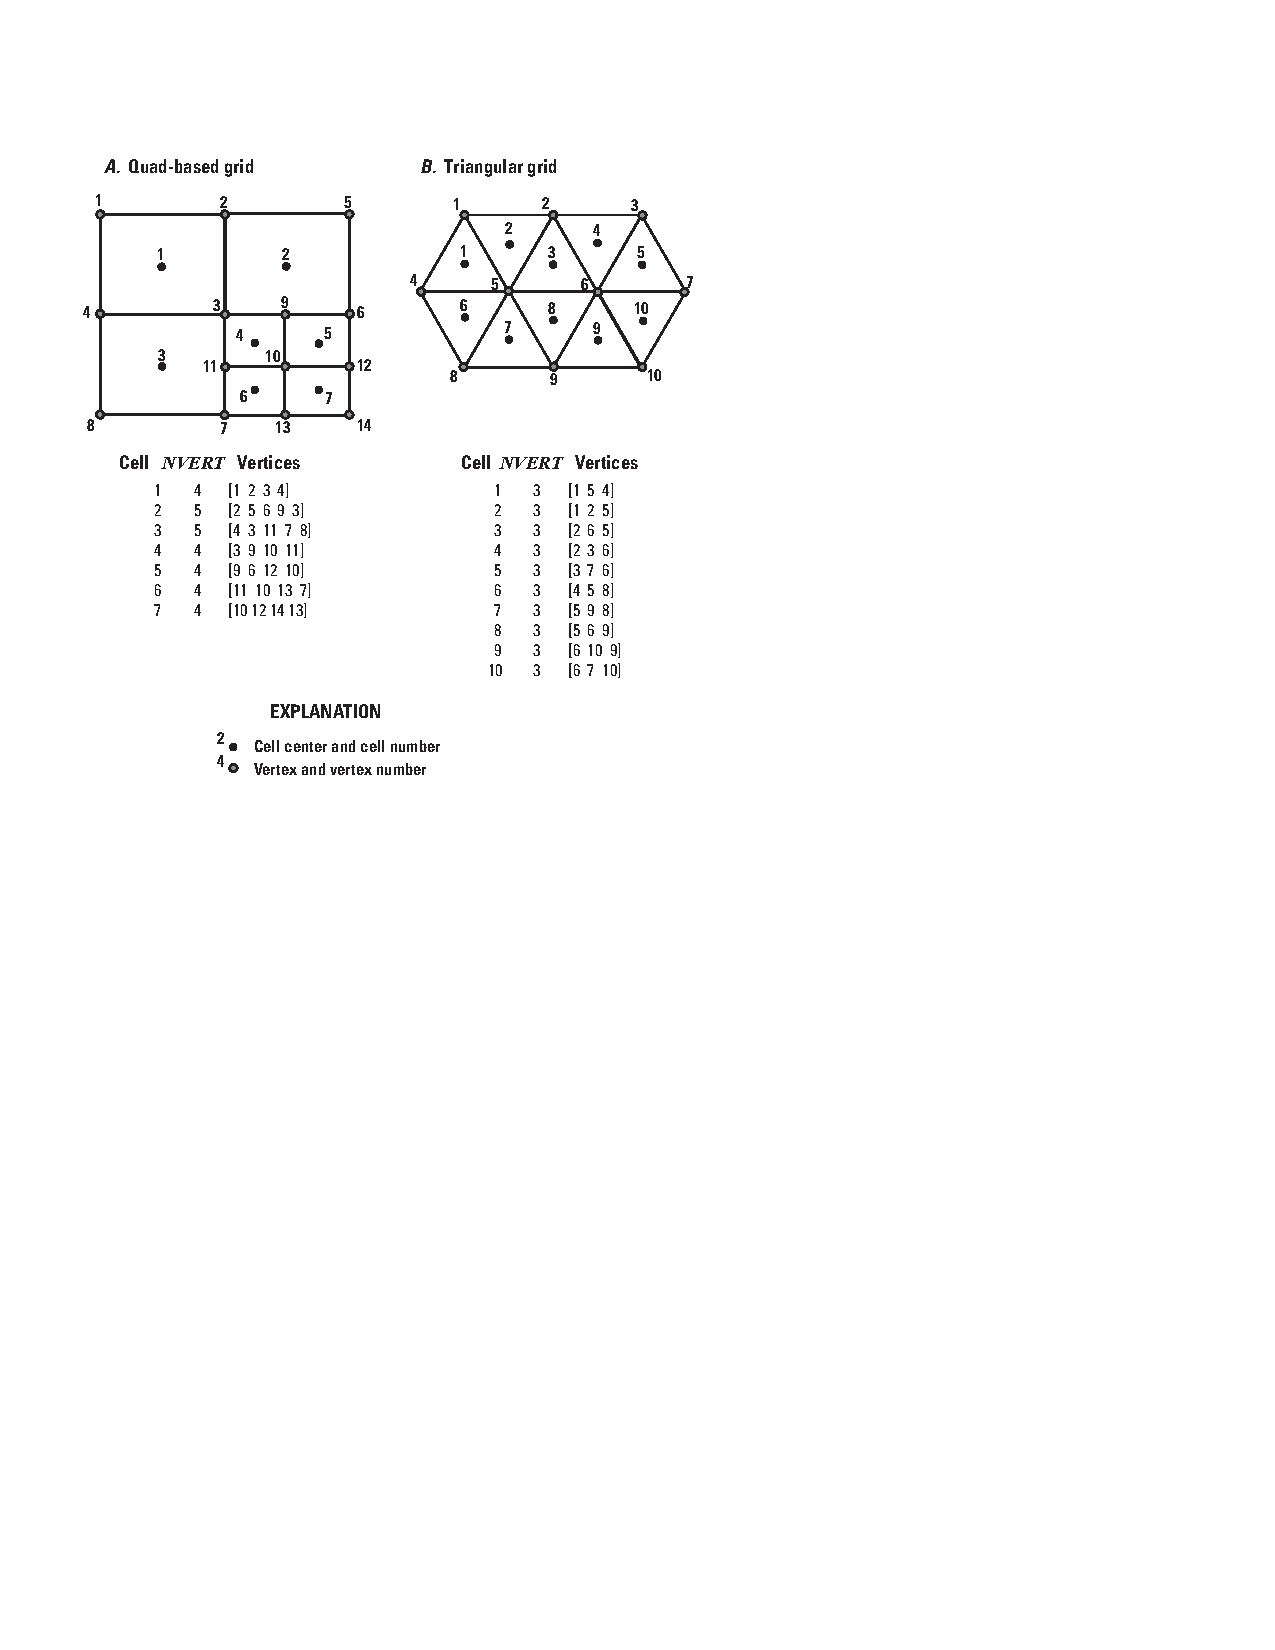
\includegraphics[scale=1.0]{Figures/gwf-fig3-2}
	\caption{Schematic diagram showing the vertices and cells defined using the Discretization by Vertices Package. The list of vertices used to define each cell must be in clockwise order.  From \cite{modflow6gwf}}
	\label{fig:gwf-fig3-2}
\end{figure}


\vspace{5mm}
\subsubsection{Structure of Blocks}
\lstinputlisting[style=blockdefinition]{./mf6ivar/tex/gwf-disv-options.dat}
\lstinputlisting[style=blockdefinition]{./mf6ivar/tex/gwf-disv-dimensions.dat}
\lstinputlisting[style=blockdefinition]{./mf6ivar/tex/gwf-disv-griddata.dat}
\lstinputlisting[style=blockdefinition]{./mf6ivar/tex/gwf-disv-vertices.dat}
\lstinputlisting[style=blockdefinition]{./mf6ivar/tex/gwf-disv-cell2d.dat}

\vspace{5mm}
\subsubsection{Explanation of Variables}
\begin{description}
\input{./mf6ivar/tex/gwf-disv-desc.tex}
\end{description}

\vspace{5mm}
\subsubsection{Example Input File}
\lstinputlisting[style=inputfile]{./mf6ivar/examples/gwf-disv-example.dat}


\newpage
\subsection{Unstructured Discretization (DISU) Input File}
Discretization information for unstructured grids is read from the file that is specified by ``DISU6'' as the file type.  Only one discretization input file (DISU6, DISV6 or DIS6) can be specified for a model.

The shape and position of each cell can be defined using vertices.  This information is optional and is only read if the number of vertices (NVERT) in the DIMENSIONS block is specified and is assigned a value larger than zero.  If the vertices and two-dimensional cell information is provided in this file, then this information is also written to the binary grid file.  Providing this information may be useful for other postprocessing programs that read the binary grid file.

\vspace{5mm}
\subsubsection{Structure of Blocks}
\lstinputlisting[style=blockdefinition]{./mf6ivar/tex/gwf-disu-options.dat}
\lstinputlisting[style=blockdefinition]{./mf6ivar/tex/gwf-disu-dimensions.dat}
\lstinputlisting[style=blockdefinition]{./mf6ivar/tex/gwf-disu-griddata.dat}
\lstinputlisting[style=blockdefinition]{./mf6ivar/tex/gwf-disu-connectiondata.dat}
\lstinputlisting[style=blockdefinition]{./mf6ivar/tex/gwf-disu-vertices.dat}
\lstinputlisting[style=blockdefinition]{./mf6ivar/tex/gwf-disu-cell2d.dat}

\vspace{5mm}
\subsubsection{Explanation of Variables}
\begin{description}
\input{./mf6ivar/tex/gwf-disu-desc.tex}
\end{description}

\vspace{5mm}
\subsubsection{Example Input File}
\lstinputlisting[style=inputfile]{./mf6ivar/examples/gwf-disu-example.dat}



\newpage
\subsection{Initial Conditions (IC) Package}
Initial Conditions (IC) Package information is read from the file that is specified by ``IC6'' as the file type.  Only one IC Package can be specified for a GWF model. 

\vspace{5mm}
\subsubsection{Structure of Blocks}
%\lstinputlisting[style=blockdefinition]{./mf6ivar/tex/gwf-ic-options.dat}
\lstinputlisting[style=blockdefinition]{./mf6ivar/tex/gwf-ic-griddata.dat}

\vspace{5mm}
\subsubsection{Explanation of Variables}
\begin{description}
\input{./mf6ivar/tex/gwf-ic-desc.tex}
\end{description}

\vspace{5mm}
\subsubsection{Example Input File}
\lstinputlisting[style=inputfile]{./mf6ivar/examples/gwf-ic-example.dat}



\newpage
\subsection{Output Control (OC) Option}
Input to the Output Control Option of the Groundwater Flow Model is read from the file that is specified as type ``OC6'' in the Name File. If no ``OC6'' file is specified, default output control is used. The Output Control Option determines how and when heads are printed to the listing file and/or written to a separate binary output file.  Under the default, head and overall budget are written to the Listing File at the end of every stress period. The default printout format for head is 10G11.4.

Output Control data must be specified using words.  The numeric codes supported in earlier MODFLOW versions can no longer be used.

All budget output is saved in the "COMPACT BUDGET" form.  COMPACT BUDGET indicates that the cell-by-cell budget file(s) will be written in a more compact form than is used in the 1988 version of MODFLOW (McDonald and Harbaugh, 1988); however, programs that read these data in the form written by MODFLOW-88 will be unable to read the new compact file. 

For the PRINT and SAVE options of heads, there is no longer an option to specify individual layers.  Whenever one of these arrays is printed or saved, all layers are printed or saved.

\vspace{5mm}
\subsubsection{Structure of Blocks}
\vspace{5mm}

\noindent \textit{FOR EACH SIMULATION}
\lstinputlisting[style=blockdefinition]{./mf6ivar/tex/gwf-oc-options.dat}
\vspace{5mm}
\noindent \textit{FOR ANY STRESS PERIOD}
\lstinputlisting[style=blockdefinition]{./mf6ivar/tex/gwf-oc-period.dat}

\vspace{5mm}
\subsubsection{Explanation of Variables}
\begin{description}
\input{./mf6ivar/tex/gwf-oc-desc.tex}
\end{description}

\vspace{5mm}
\subsubsection{Example Input File}
\lstinputlisting[style=inputfile]{./mf6ivar/examples/gwf-oc-example.dat}


\newpage
\subsection{Observation (OBS) Utility for a GWF Model}
GWF & head & cellid & -- & Head at a specified cell. \\
GWF & drawdown & cellid & -- & Drawdown at a specified cell calculated as difference between starting head and simulated head for the time step. \\
GWF & flow-ja-face & cellid & cellid & Flow between two adjacent cells.

\newpage
\subsection{Node Property Flow (NPF) Package}
Input to the Node Property Flow (NPF) Package is read from the file that has type ``NPF6'' in the Name File.  A single NPF Package is required for each GWF model. 

\vspace{5mm}
\subsubsection{Structure of Blocks}
\lstinputlisting[style=blockdefinition]{./mf6ivar/tex/gwf-npf-options.dat}
\lstinputlisting[style=blockdefinition]{./mf6ivar/tex/gwf-npf-griddata.dat}

\vspace{5mm}
\subsubsection{Explanation of Variables}
\begin{description}
\input{./mf6ivar/tex/gwf-npf-desc.tex}
\end{description}

\vspace{5mm}
\subsubsection{Example Input File}
\lstinputlisting[style=inputfile]{./mf6ivar/examples/gwf-npf-example.dat}



\newpage
\subsection{Horizontal Flow Barrier (HFB) Package}
Input to the Horizontal Flow Barrier (HFB) Package is read from the file that has type ``HFB6'' in the Name File.  Only one HFB Package can be specified for a GWF model.

\vspace{5mm}
\subsubsection{Structure of Blocks}
\vspace{5mm}

\noindent \textit{FOR EACH SIMULATION}
\lstinputlisting[style=blockdefinition]{./mf6ivar/tex/gwf-hfb-options.dat}
\lstinputlisting[style=blockdefinition]{./mf6ivar/tex/gwf-hfb-dimensions.dat}
\vspace{5mm}
\noindent \textit{FOR ANY STRESS PERIOD}
\lstinputlisting[style=blockdefinition]{./mf6ivar/tex/gwf-hfb-period.dat}

\vspace{5mm}
\subsubsection{Explanation of Variables}
\begin{description}
\input{./mf6ivar/tex/gwf-hfb-desc.tex}
\end{description}

\vspace{5mm}
\subsubsection{Example Input File}
\lstinputlisting[style=inputfile]{./mf6ivar/examples/gwf-hfb-example.dat}


\newpage
\subsection{Storage (STO) Package}
Input to the Storage (STO) Package is read from the file that has type ``STO6'' in the Name File.  If the STO Package is not included for a model, then storage changes will not be calculated, and thus, the model will be steady state.  Only one STO Package can be specified for a GWF model.

\vspace{5mm}
\subsubsection{Structure of Blocks}

\vspace{5mm}
\noindent \textit{FOR EACH SIMULATION}
\lstinputlisting[style=blockdefinition]{./mf6ivar/tex/gwf-sto-options.dat}
\lstinputlisting[style=blockdefinition]{./mf6ivar/tex/gwf-sto-griddata.dat}
\vspace{5mm}
\noindent \textit{FOR ANY STRESS PERIOD}
\lstinputlisting[style=blockdefinition]{./mf6ivar/tex/gwf-sto-period.dat}

\vspace{5mm}
\subsubsection{Explanation of Variables}
\begin{description}
\input{./mf6ivar/tex/gwf-sto-desc.tex}
\end{description}

\vspace{5mm}
\subsubsection{Example Input File}
\lstinputlisting[style=inputfile]{./mf6ivar/examples/gwf-sto-example.dat}



\newpage
\subsection{Constant-Head (CHD) Package}

Input to the Constant-Head (CHD) Package is read from the file that has type ``CHD6'' in the Name File.  Any number of CHD Packages can be specified for a single groundwater flow model; however, an error will occur if a CHD Package attempts to make a GWF cell a constant-head cell when that cell has already been designated as a constant-head cell either within the present CHD Package or within another CHD Package.  All single valued variables are free format.  

In previous MODFLOW versions, it was not possible to convert a constant-head cell to an active cell.  Once a cell was designated as a constant-head cell, it remained a constant-head cell until the end of the end of the simulation.  In \mf a constant-head cell will become active again if it is not included as a constant-head cell in subsequent stress periods.

Previous MODFLOW versions allowed specification of SHEAD and EHEAD, which were the starting and ending prescribed heads for a stress period.  Linear interpolation was used to calculate a value for each time step.  In \mf only a single head value can be specified for any constant-head cell in any stress period.  The time-series functionality must be used in order to interpolate values to individual time steps.  

\vspace{5mm}
\subsubsection{Structure of Blocks}
\vspace{5mm}

\noindent \textit{FOR EACH SIMULATION}
\lstinputlisting[style=blockdefinition]{./mf6ivar/tex/gwf-chd-options.dat}
\lstinputlisting[style=blockdefinition]{./mf6ivar/tex/gwf-chd-dimensions.dat}
\vspace{5mm}
\noindent \textit{FOR ANY STRESS PERIOD}
\lstinputlisting[style=blockdefinition]{./mf6ivar/tex/gwf-chd-period.dat}

\vspace{5mm}
\subsubsection{Explanation of Variables}
\begin{description}
\input{./mf6ivar/tex/gwf-chd-desc.tex}
\end{description}

\vspace{5mm}
\subsubsection{Example Input File}
\lstinputlisting[style=inputfile]{./mf6ivar/examples/gwf-chd-example.dat}

\vspace{5mm}
\subsubsection{Available observation types}
CHD Package observations are limited to the simulated constant head flow rate (\texttt{chd}). The data required for the CHD Package observation type is defined in table~\ref{table:gwf-chdobstype}. Negative and positive values for an observation represent a loss from and gain to the GWF model, respectively.

\begin{longtable}{p{2cm} p{2.75cm} p{2cm} p{1.25cm} p{7cm}}
\caption{Available CHD Package observation types} \tabularnewline

\hline
\hline
\textbf{Model} & \textbf{Observation type} & \textbf{ID} & \textbf{ID2} & \textbf{Description} \\
\hline
\endhead

\hline
\endfoot

\input{../Common/gwf-chdobs.tex}
\label{table:gwf-chdobstype}
\end{longtable}

\vspace{5mm}
\subsubsection{Example Observation Input File}
\lstinputlisting[style=inputfile]{./mf6ivar/examples/gwf-chd-example-obs.dat}



\newpage
\subsection{Well (WEL) Package}
Input to the Well (WEL) Package is read from the file that has type ``WEL6'' in the Name File.  Any number of WEL Packages can be specified for a single groundwater flow model.  All single valued variables are free format.

\vspace{5mm}
\subsubsection{Structure of Blocks}
\vspace{5mm}

\noindent \textit{FOR EACH SIMULATION}
\lstinputlisting[style=blockdefinition]{./mf6ivar/tex/gwf-wel-options.dat}
\lstinputlisting[style=blockdefinition]{./mf6ivar/tex/gwf-wel-dimensions.dat}
\vspace{5mm}
\noindent \textit{FOR ANY STRESS PERIOD}
\lstinputlisting[style=blockdefinition]{./mf6ivar/tex/gwf-wel-period.dat}

\vspace{5mm}
\subsubsection{Explanation of Variables}
\begin{description}
\input{./mf6ivar/tex/gwf-wel-desc.tex}
\end{description}

\vspace{5mm}
\subsubsection{Example Input File}
\lstinputlisting[style=inputfile]{./mf6ivar/examples/gwf-wel-example.dat}

\vspace{5mm}
\subsubsection{Available observation types}
Well Package observations include the simulated well rates (\texttt{wel}) and the well discharge that is available for the MVR package (\texttt{to-mvr}). The data required for each WEL Package observation type is defined in table~\ref{table:gwf-welobstype}. The sum of \texttt{wel} and \texttt{to-mvr} is equal to the simulated well discharge rate, which may be less than the specified \texttt{q} if the \texttt{AUTO\_FLOW\_REDUCE} option is enabled. Negative and positive values for an observation represent a loss from and gain to the GWF model, respectively.

\begin{longtable}{p{2cm} p{2.75cm} p{2cm} p{1.25cm} p{7cm}}
\caption{Available WEL Package observation types} \tabularnewline

\hline
\hline
\textbf{Stress Package} & \textbf{Observation type} & \textbf{ID} & \textbf{ID2} & \textbf{Description} \\
\hline
\endhead

\hline
\endfoot

\input{../Common/gwf-welobs.tex}
\label{table:gwf-welobstype}
\end{longtable}

\vspace{5mm}
\subsubsection{Example Observation Input File}
\lstinputlisting[style=inputfile]{./mf6ivar/examples/gwf-wel-example-obs.dat}


\newpage
\subsection{Drain (DRN) Package}
Input to the Drain (DRN) Package is read from the file that has type ``DRN6'' in the Name File.  Any number of DRN Packages can be specified for a single groundwater flow model.  All single valued variables are free format.

\vspace{5mm}
\subsubsection{Structure of Blocks}
\vspace{5mm}

\noindent \textit{FOR EACH SIMULATION}
\lstinputlisting[style=blockdefinition]{./mf6ivar/tex/gwf-drn-options.dat}
\lstinputlisting[style=blockdefinition]{./mf6ivar/tex/gwf-drn-dimensions.dat}
\vspace{5mm}
\noindent \textit{FOR ANY STRESS PERIOD}
\lstinputlisting[style=blockdefinition]{./mf6ivar/tex/gwf-drn-period.dat}

\vspace{5mm}
\subsubsection{Explanation of Variables}
\begin{description}
\input{./mf6ivar/tex/gwf-drn-desc.tex}
\end{description}

\vspace{5mm}
\subsubsection{Example Input File}
\lstinputlisting[style=inputfile]{./mf6ivar/examples/gwf-drn-example.dat}

\vspace{5mm}
\subsubsection{Available observation types}
Drain Package observations include the simulated drain rates (\texttt{drn}) and the drain discharge that is available for the MVR package (\texttt{to-mvr}). The data required for each DRN Package observation type is defined in table~\ref{table:gwf-drnobstype}. The sum of \texttt{drn} and \texttt{to-mvr} is equal to the simulated drain discharge rate for a drain boundary or group of drain boundaries.

\begin{longtable}{p{2cm} p{2.75cm} p{2cm} p{1.25cm} p{7cm}}
\caption{Available DRN Package observation types} \tabularnewline

\hline
\hline
\textbf{Model} & \textbf{Observation type} & \textbf{ID} & \textbf{ID2} & \textbf{Description} \\
\hline
\endhead

\hline
\endfoot

DRN & drn & cellid or boundname & -- & Flow between the groundwater system and a drain boundary or group of drain boundaries. \\
DRN & to-mvr & cellid or boundname & -- & Drain boundary discharge that is available for the MVR package for a drain boundary or a group of drain boundaries.
\label{table:gwf-drnobstype}
\end{longtable}

\vspace{5mm}
\subsubsection{Example Observation Input File}
\lstinputlisting[style=inputfile]{./mf6ivar/examples/gwf-drn-example-obs.dat}


\newpage
\subsection{River (RIV) Package}
Input to the River (RIV) Package is read from the file that has type ``RIV6'' in the Name File.  Any number of RIV Packages can be specified for a single groundwater flow model.  All single valued variables are free format.

\vspace{5mm}
\subsubsection{Structure of Blocks}
\vspace{5mm}

\noindent \textit{FOR EACH SIMULATION}
\lstinputlisting[style=blockdefinition]{./mf6ivar/tex/gwf-riv-options.dat}
\lstinputlisting[style=blockdefinition]{./mf6ivar/tex/gwf-riv-dimensions.dat}
\vspace{5mm}
\noindent \textit{FOR ANY STRESS PERIOD}
\lstinputlisting[style=blockdefinition]{./mf6ivar/tex/gwf-riv-period.dat}

\vspace{5mm}
\subsubsection{Explanation of Variables}
\begin{description}
\input{./mf6ivar/tex/gwf-riv-desc.tex}
\end{description}

\vspace{5mm}
\subsubsection{Example Input File}
\lstinputlisting[style=inputfile]{./mf6ivar/examples/gwf-riv-example.dat}

\vspace{5mm}
\subsubsection{Available observation types}
River Package observations include the simulated river flow rates (\texttt{riv}) and the river discharge that is available for the MVR package (\texttt{to-mvr}). The data required for each RIV Package observation type is defined in table~\ref{table:gwf-rivobstype}. The sum of \texttt{riv} and \texttt{to-mvr} is equal to the simulated river flow rate. Negative and positive values for an observation represent a loss from and gain to the GWF model, respectively.

\begin{longtable}{p{2cm} p{2.75cm} p{2cm} p{1.25cm} p{7cm}}
\caption{Available RIV Package observation types} \tabularnewline

\hline
\hline
\textbf{Stress Package} & \textbf{Observation type} & \textbf{ID} & \textbf{ID2} & \textbf{Description} \\
\hline
\endfirsthead

\hline
\hline
\textbf{Stress Package} & \textbf{Observation type} & \textbf{ID} & \textbf{ID2} & \textbf{Description} \\
\hline
\endhead

\hline
\endfoot

\input{../Common/gwf-rivobs.tex}
\label{table:gwf-rivobstype}
\end{longtable}

\vspace{5mm}
\subsubsection{Example Observation Input File}
\lstinputlisting[style=inputfile]{./mf6ivar/examples/gwf-riv-example-obs.dat}


\newpage
\subsection{General-Head Boundary (GHB) Package}
Input to the General-Head Boundary (GHB) Package is read from the file that has type ``GHB6'' in the Name File.  Any number of GHB Packages can be specified for a single groundwater flow model.  All single valued variables are free format.

\vspace{5mm}
\subsubsection{Structure of Blocks}
\vspace{5mm}

\noindent \textit{FOR EACH SIMULATION}
\lstinputlisting[style=blockdefinition]{./mf6ivar/tex/gwf-ghb-options.dat}
\lstinputlisting[style=blockdefinition]{./mf6ivar/tex/gwf-ghb-dimensions.dat}
\vspace{5mm}
\noindent \textit{FOR ANY STRESS PERIOD}
\lstinputlisting[style=blockdefinition]{./mf6ivar/tex/gwf-ghb-period.dat}

\vspace{5mm}
\subsubsection{Explanation of Variables}
\begin{description}
\input{./mf6ivar/tex/gwf-ghb-desc.tex}
\end{description}

\vspace{5mm}
\subsubsection{Example Input File}
\lstinputlisting[style=inputfile]{./mf6ivar/examples/gwf-ghb-example.dat}

\vspace{5mm}
\subsubsection{Available observation types}
General-Head Boundary Package observations include the simulated general-head boundary flow rates (\texttt{ghb}) and the general-head boundary discharge that is available for the MVR package (\texttt{to-mvr}). The data required for each GHB Package observation type is defined in table~\ref{table:gwf-ghbobstype}. The sum of \texttt{ghb} and \texttt{to-mvr} is equal to the simulated general-head boundary flow rate. Negative and positive values for an observation represent a loss from and gain to the GWF model, respectively.

\begin{longtable}{p{2cm} p{2.75cm} p{2cm} p{1.25cm} p{7cm}}
\caption{Available GHB Package observation types} \tabularnewline

\hline
\hline
\textbf{Stress Package} & \textbf{Observation type} & \textbf{ID} & \textbf{ID2} & \textbf{Description} \\
\hline
\endhead

\hline
\endfoot

\input{../Common/gwf-ghbobs.tex}
\label{table:gwf-ghbobstype}
\end{longtable}

\vspace{5mm}
\subsubsection{Example Observation Input File}
\lstinputlisting[style=inputfile]{./mf6ivar/examples/gwf-ghb-example-obs.dat}


\newpage
\subsection{Recharge (RCH) Package -- List-Based Input}

Input to the Recharge (RCH) Package is read from the file that has type ``RCH6'' in the Name File.  Any number of RCH Packages can be specified for a single groundwater flow model.  All single valued variables are free format. 

Recharge input can be specified using lists or arrays, unless the DISU Package is used.  List-based input must be used if discretization is specified using the DISU Package.  List-based input for recharge is the default, and is described here.  Instructions for specifying array-based recharge are described in the next section. 

List-based input offers several advantages over the array-based input for specifying recharge.  First, multiple list entries can be specified for a single cell.  This makes it possible to divide a cell into multiple areas, and assign a different recharge rate for each area (perhaps based on land use or some other criteria).  In this case, the user would likely specify an auxiliary variable to serve as a multiplier.  This multiplier would be calculated by the user and provided in the input file as the fractional cell are for the individual recharge entries.  Another advantage to using list-based input for specifying recharge is that boundnames can be specified.  Boundnames work with the Observations capability and can be used to sum recharge rates for entries with the same boundname.  A disadvantage of the list-based input is that one cannot easily assign recharge to the entire model without specifying a list of model cells.  For this reason \mf also supports array-based input for recharge.

\vspace{5mm}
\subsubsection{Structure of Blocks}
\vspace{5mm}

\noindent \textit{FOR EACH SIMULATION}
\lstinputlisting[style=blockdefinition]{./mf6ivar/tex/gwf-rch-options.dat}
\lstinputlisting[style=blockdefinition]{./mf6ivar/tex/gwf-rch-dimensions.dat}
\vspace{5mm}
\noindent \textit{FOR ANY STRESS PERIOD}
\lstinputlisting[style=blockdefinition]{./mf6ivar/tex/gwf-rch-period.dat}

\vspace{5mm}
\subsubsection{Explanation of Variables}
\begin{description}
\input{./mf6ivar/tex/gwf-rch-desc.tex}
\end{description}

\vspace{5mm}
\subsubsection{Example Input File}
\lstinputlisting[style=inputfile]{./mf6ivar/examples/gwf-rch-example.dat}

\vspace{5mm}
\subsubsection{Available observation types}
Recharge Package observations are limited to the simulated recharge flow rates (\texttt{rch}). The data required for the RCH Package observation type is defined in table~\ref{table:gwf-rchobstype}. Negative and positive values for an observation represent a loss from and gain to the GWF model, respectively.

\begin{longtable}{p{2cm} p{2.75cm} p{2cm} p{1.25cm} p{7cm}}
\caption{Available RCH Package observation types} \tabularnewline

\hline
\hline
\textbf{Stress Package} & \textbf{Observation type} & \textbf{ID} & \textbf{ID2} & \textbf{Description} \\
\hline
\endhead

\hline
\endfoot

\input{../Common/gwf-rchobs.tex}
\label{table:gwf-rchobstype}
\end{longtable}

\vspace{5mm}
\subsubsection{Example Observation Input File}
\lstinputlisting[style=inputfile]{./mf6ivar/examples/gwf-rch-example-obs.dat}


\newpage
\subsection{Recharge (RCH) Package -- Array-Based Input}

Input to the Recharge (RCH) Package is read from the file that has type ``RCH6'' in the Name File.  Any number of RCH Packages can be specified for a single groundwater flow model.  All single valued variables are free format. 

Recharge input can be specified using lists or arrays.  Array-based input for recharge is activated by providing READASARRAYS within the OPTIONS block.   Instructions for specifying list-based recharge is described in the previous section.  Array-based input for recharge provides a similar approach for providing recharge rates as previous MODFLOW versions.  Array-based input for recharge can be used only with the DIS and DISV Packages.  Array-based input for recharge cannot be used with the DISU Package.

When array-based input is used for recharge, the DIMENSIONS block should not be specified.  The array size is determined from the model grid. 

\vspace{5mm}
\subsubsection{Structure of Blocks}
\vspace{5mm}

\noindent \textit{FOR EACH SIMULATION}
\lstinputlisting[style=blockdefinition]{./mf6ivar/tex/gwf-rcha-options.dat}
\vspace{5mm}
\noindent \textit{FOR ANY STRESS PERIOD}
\lstinputlisting[style=blockdefinition]{./mf6ivar/tex/gwf-rcha-period.dat}

\vspace{5mm}
\subsubsection{Explanation of Variables}
\begin{description}
\input{./mf6ivar/tex/gwf-rcha-desc.tex}
\end{description}

\vspace{5mm}
\subsubsection{Example Input File}
\lstinputlisting[style=inputfile]{./mf6ivar/examples/gwf-rcha-example.dat}



\newpage
\subsection{Evapotranspiration (EVT) Package -- List-Based Input}
Input to the Evapotranspiration (EVT) Package is read from the file that has type ``EVT6'' in the Name File. Any number of EVT Packages can be specified for a single groundwater flow model. All single-valued variables are free format.

Evapotranspiration input can be specified using lists or arrays, unless the DISU Package is used.  List-based input must be used if discretization is specified using the DISU Package.  List-based input for recharge is the default, and is described here.  Instructions for specifying array-based recharge are described in the next section. 

List-based input offers several advantages over the array-based input for specifying evapotranspiration.  First, multiple list entries can be specified for a single cell.  This makes it possible to divide a cell into multiple areas, and assign a different evapotranspiration rate or extinction depth for each area (perhaps based on vegetation type or some other criteria).  In this case, the user would likely specify an auxiliary variable to serve as a multiplier.  This multiplier would be calculated by the user and provided in the input file as the fractional cell are for the individual evapotranspiration entries.  Another advantage to using list-based input for specifying evapotranspiration is that boundnames can be specified.  Boundnames work with the Observations capability and can be used to sum evapotranspiration rates for entries with the same boundname.  A disadvantage of the list-based input is that one cannot easily assign evapotranspiration to the entire model without specifying a list of model cells.  For this reason \mf also supports array-based input for evapotranspiration.

ET input is read in list form, as shown in the PERIOD block below. Each line in the PERIOD block defines all input for one cell. Entries following \texttt{cellid}, in order, define the ET surface (\texttt{etss}), maximum ET flux rate (\texttt{etsr}), extinction depth (\texttt{etsx}), all (\texttt{netseg} -- 1) \texttt{pxdp} values, all (\texttt{netseg} -- 1) \texttt{petm} values, all auxiliary variables (if AUXILIARY option is specified), and boundary name (if BOUNDNAMES option is specified).

\vspace{5mm}
\subsubsection{Structure of Blocks}
\vspace{5mm}

\noindent \textit{FOR EACH SIMULATION}
\lstinputlisting[style=blockdefinition]{./mf6ivar/tex/gwf-evt-options.dat}
\lstinputlisting[style=blockdefinition]{./mf6ivar/tex/gwf-evt-dimensions.dat}
\vspace{5mm}
\noindent \textit{FOR ANY STRESS PERIOD}
\lstinputlisting[style=blockdefinition]{./mf6ivar/tex/gwf-evt-period.dat}

\vspace{5mm}
\subsubsection{Explanation of Variables}
\begin{description}
\input{./mf6ivar/tex/gwf-evt-desc.tex}
\end{description}

\vspace{5mm}
\subsubsection{Example Input File}
\lstinputlisting[style=inputfile]{./mf6ivar/examples/gwf-evt-example.dat}

\vspace{5mm}
\subsubsection{Available observation types}
Evapotranspiration Package observations are limited to the simulated evapotranspiration flow rates (\texttt{evt}). The data required for the EVT Package observation type is defined in table~\ref{table:gwf-evtobstype}. Negative and positive values for an observation represent a loss from and gain to the GWF model, respectively.

\begin{longtable}{p{2cm} p{2.75cm} p{2cm} p{1.25cm} p{7cm}}
\caption{Available EVT Package observation types} \tabularnewline

\hline
\hline
\textbf{Stress Package} & \textbf{Observation type} & \textbf{ID} & \textbf{ID2} & \textbf{Description} \\
\hline
\endhead

\hline
\endfoot

\input{../Common/gwf-evtobs.tex}
\label{table:gwf-evtobstype}
\end{longtable}

\vspace{5mm}
\subsubsection{Example Observation Input File}
\lstinputlisting[style=inputfile]{./mf6ivar/examples/gwf-evt-example-obs.dat}


\newpage
\subsection{Evapotranspiration (EVT) Package -- Array-Based Input}
Input to the Evapotranspiration (EVT) Package is read from the file that has type ``EVT6'' in the Name File. Any number of EVT Packages can be specified for a single groundwater flow model. All single-valued variables are free format.

Evapotranspiration input can be specified using lists or arrays.  Array-based input for evapotranspiration is activated by providing READASARRAYS within the OPTIONS block.   Instructions for specifying list-based evapotranspiration is described in the previous section.  Array-based input for evapotranspiration provides a similar approach for providing evapotranspiration rates as previous MODFLOW versions.  Array-based input for evapotranspiration can be used only with the DIS and DISV Packages.  Array-based input for evapotranspiration cannot be used with the DISU Package.

When array-based input is used for evapotranspiration, the DIMENSIONS block should not be specified.  The array size is determined from the model grid.   Segmented evapotranspiration cannot be used with the READASARRAYS option.

\vspace{5mm}
\subsubsection{Structure of Blocks}
\vspace{5mm}

\noindent \textit{FOR EACH SIMULATION}
\lstinputlisting[style=blockdefinition]{./mf6ivar/tex/gwf-evta-options.dat}
\vspace{5mm}
\noindent \textit{FOR ANY STRESS PERIOD}
\lstinputlisting[style=blockdefinition]{./mf6ivar/tex/gwf-evta-period.dat}

\vspace{5mm}
\subsubsection{Explanation of Variables}
\begin{description}
\input{./mf6ivar/tex/gwf-evta-desc.tex}
\end{description}

\vspace{5mm}
\subsubsection{Example Input File}
\lstinputlisting[style=inputfile]{./mf6ivar/examples/gwf-evta-example.dat}


\newpage
\subsection{Multi-Aquifer Well (MAW) Package}
Input to the Multi-Aquifer Well (MAW) Package is read from the file that has type ``MAW6'' in the Name File.  Any number of MAW Packages can be specified for a single groundwater flow model.  All single valued variables are free format.

\vspace{5mm}
\subsubsection{Structure of Blocks}
\vspace{5mm}

\noindent \textit{FOR EACH SIMULATION}
\lstinputlisting[style=blockdefinition]{./mf6ivar/tex/gwf-maw-options.dat}
\lstinputlisting[style=blockdefinition]{./mf6ivar/tex/gwf-maw-dimensions.dat}
\lstinputlisting[style=blockdefinition]{./mf6ivar/tex/gwf-maw-packagedata.dat}
\lstinputlisting[style=blockdefinition]{./mf6ivar/tex/gwf-maw-connectiondata.dat}
\vspace{5mm}
\noindent \textit{FOR ANY STRESS PERIOD}
\lstinputlisting[style=blockdefinition]{./mf6ivar/tex/gwf-maw-period.dat}

\vspace{5mm}
\subsubsection{Explanation of Variables}
\begin{description}
\input{./mf6ivar/tex/gwf-maw-desc.tex}
\end{description}

\vspace{5mm}
\subsubsection{Example Input File -- Conductance Calculated using Thiem Equation}
\lstinputlisting[style=inputfile]{./mf6ivar/examples/gwf-maw-example1.dat}
\subsubsection{Example Input File -- Conductance Calculated using Screen Geometry}
\lstinputlisting[style=inputfile]{./mf6ivar/examples/gwf-maw-example2.dat}
\subsubsection{Example Input File -- Flowing Well with Conductance Specified}
\lstinputlisting[style=inputfile]{./mf6ivar/examples/gwf-maw-example3.dat}

\vspace{5mm}
\subsubsection{Available observation types}
Multi-Aquifer Well Package observations include well head and all of the terms that contribute to the continuity equation for each multi-aquifer well. Additional LAK Package observations include the conductance for a well-aquifer connection conductance (\texttt{conductance}) and the calculated flowing well-aquifer connection conductance (\texttt{fw-conductance}). The data required for each MAW Package observation type is defined in table~\ref{table:gwf-mawobstype}. Negative and positive values for \texttt{maw} observations represent a loss from and gain to the GWF model, respectively. For all other flow terms, negative and positive values represent a loss from and gain from the MAW package, respectively.

\begin{longtable}{p{2cm} p{2.75cm} p{2cm} p{1.25cm} p{7cm}}
\caption{Available MAW Package observation types} \tabularnewline

\hline
\hline
\textbf{Stress Package} & \textbf{Observation type} & \textbf{ID} & \textbf{ID2} & \textbf{Description} \\
\hline
\endfirsthead

\captionsetup{textformat=simple}
\caption*{\textbf{Table \arabic{table}.}{\quad}Available MAW Package observation types.---Continued} \\

\hline
\hline
\textbf{Stress Package} & \textbf{Observation type} & \textbf{ID} & \textbf{ID2} & \textbf{Description} \\
\hline
\endhead

\hline
\endfoot

\input{../Common/gwf-mawobs.tex}
\label{table:gwf-mawobstype}
\end{longtable}

\vspace{5mm}
\subsubsection{Example Observation Input File}
\lstinputlisting[style=inputfile]{./mf6ivar/examples/gwf-maw-example-obs.dat}


\newpage
\subsection{Streamflow Routing (SFR) Package}
Input to the Streamflow Routing (SFR) Package is read from the file that has type ``SFR6'' in the Name File. Any number of SFR Packages can be specified for a single groundwater flow model; however, water cannot be routed between reaches in separate packages except in cases where the MVR Package is used to route water between separate packages. All single valued variables are free format.

Reach connectivity must be explicitly specified for this version of the SFR Package, unlike the abbreviated SFR Package segment connectivity specified in previous versions of MODFLOW. Explicit specification of reach connectivity has been adopted to facilitate better validation of stream network connectivity by the program. Explicit reach connectivity means that a reach must be specified as an upstream connection for all downstream connections to the reach. Downstream connections for a reach are denoted with a negative reach number. Flow in a reach is unidirectional, always flowing from the upstream end to the downstream end of a reach. An example of the reach connectivity for a hypothetical stream network is shown in figure~\ref{fig:sfr-connectivity}.

\begin{figure}[ht]
	\centering
	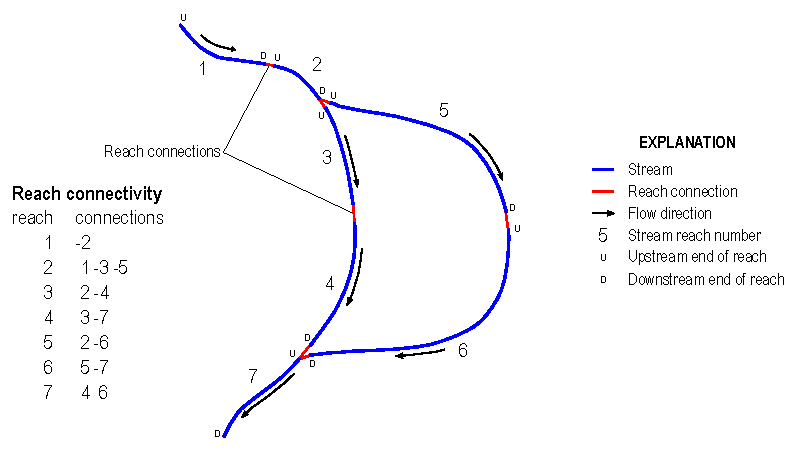
\includegraphics[scale=1.0]{../Figures/sfr-connectivity}
	\caption[Illustration of a simple stream network having seven reaches with a junction having two reaches, a confluence of two reaches, and the resulting reach connectivity]{Simple stream network having seven reaches with a junction having two reaches, a confluence of two reaches, and the resulting reach connectivity. Downstream connections for a reach must include the reach as an upstream connection for all downstream connections to the reach. Downstream connections for a  reach are denoted with a negative reach number}
	\label{fig:sfr-connectivity}
\end{figure}


\vspace{5mm}
\subsubsection{Structure of Blocks}
\vspace{5mm}

\noindent \textit{FOR EACH SIMULATION}
\lstinputlisting[style=blockdefinition]{./mf6ivar/tex/gwf-sfr-options.dat}
\lstinputlisting[style=blockdefinition]{./mf6ivar/tex/gwf-sfr-dimensions.dat}
\lstinputlisting[style=blockdefinition]{./mf6ivar/tex/gwf-sfr-packagedata.dat}
\lstinputlisting[style=blockdefinition]{./mf6ivar/tex/gwf-sfr-connectiondata.dat}
\noindent \textit{IF \texttt{ndv} IS GREATER THAN ZERO FOR ANY REACH}
\lstinputlisting[style=blockdefinition]{./mf6ivar/tex/gwf-sfr-diversions.dat}

\vspace{5mm}
\noindent \textit{FOR ANY STRESS PERIOD}
\lstinputlisting[style=blockdefinition]{./mf6ivar/tex/gwf-sfr-period.dat}

\vspace{5mm}
\subsubsection{Explanation of Variables}
\begin{description}
\input{./mf6ivar/tex/gwf-sfr-desc.tex}
\end{description}

\vspace{5mm}
\subsubsection{Example Input File}
\lstinputlisting[style=inputfile]{./mf6ivar/examples/gwf-sfr-example.dat}

\vspace{5mm}
\subsubsection{Available observation types}
Streamflow Routing Package observations include reach stage and all of the terms that contribute to the continuity equation for each stream reach. Additional SFR Package observations include the sum of inflows from upstream reaches and from mover terms (\texttt{upstream-flow}) and downstream outflow from a reach prior to diversions and the mover package (\texttt{downstream-flow}). The data required for each SFR Package observation type is defined in table~\ref{table:gwf-sfrobstype}. Negative and positive values for \texttt{sfr} observations represent a loss from and gain to the GWF model, respectively. For all other flow terms, negative and positive values represent a loss from and gain from the SFR package, respectively.

\FloatBarrier
\begin{longtable}{p{2cm} p{2.75cm} p{2cm} p{1.25cm} p{7cm}}
\caption{Available SFR Package observation types} \tabularnewline

\hline
\hline
\textbf{Stress Package} & \textbf{Observation type} & \textbf{ID} & \textbf{ID2} & \textbf{Description} \\
\hline
\endfirsthead

\captionsetup{textformat=simple}
\caption*{\textbf{Table \arabic{table}.}{\quad}Available SFR Package observation types.---Continued} \\

\hline
\hline
\textbf{Stress Package} & \textbf{Observation type} & \textbf{ID} & \textbf{ID2} & \textbf{Description} \\
\hline
\endhead


\hline
\endfoot

\input{../Common/gwf-sfrobs.tex}
\label{table:gwf-sfrobstype}
\end{longtable}
\FloatBarrier

\vspace{5mm}
\subsubsection{Example Observation Input File}
\lstinputlisting[style=inputfile]{./mf6ivar/examples/gwf-sfr-example-obs.dat}


\newpage
\subsection{Lake (LAK) Package}
Input to the Lake (LAK) Package is read from the file that has type ``LAK6'' in the Name File.  Any number of LAK Packages can be specified for a single groundwater flow model.  All single valued variables are free format.

\vspace{5mm}
\subsubsection{Structure of Blocks}
\vspace{5mm}

\noindent \textit{FOR EACH SIMULATION}
\lstinputlisting[style=blockdefinition]{./mf6ivar/tex/gwf-lak-options.dat}
\lstinputlisting[style=blockdefinition]{./mf6ivar/tex/gwf-lak-dimensions.dat}
\lstinputlisting[style=blockdefinition]{./mf6ivar/tex/gwf-lak-packagedata.dat}
\noindent \textit{IF \texttt{nlakeconn} IS GREATER THAN ZERO FOR ANY LAKE}
\lstinputlisting[style=blockdefinition]{./mf6ivar/tex/gwf-lak-connectiondata.dat}
\noindent \textit{IF \texttt{ntables} IS GREATER THAN ZERO}
\lstinputlisting[style=blockdefinition]{./mf6ivar/tex/gwf-lak-tables.dat}
\noindent \textit{IF \texttt{noutlets} IS GREATER THAN ZERO FOR ANY LAKE}
\lstinputlisting[style=blockdefinition]{./mf6ivar/tex/gwf-lak-outlets.dat}

\vspace{5mm}
\noindent \textit{FOR ANY STRESS PERIOD}
\lstinputlisting[style=blockdefinition]{./mf6ivar/tex/gwf-lak-period.dat}

\vspace{5mm}
\subsubsection{Explanation of Variables}
\begin{description}
\input{./mf6ivar/tex/gwf-lak-desc.tex}
\end{description}

\vspace{5mm}
\subsubsection{Example Input File}
\lstinputlisting[style=inputfile]{./mf6ivar/examples/gwf-lak-example.dat}

\vspace{5mm}
\subsubsection{Available observation types}
Lake Package observations include lake stage and all of the terms that contribute to the continuity equation for each lake. Additional LAK Package observations include flow rates for individual outlets, lakes, or groups of lakes (\texttt{outlet}); the lake volume (\texttt{volume}); lake surface area (\texttt{surface-area}); wetted area for a lake-aquifer connection (\texttt{wetted-area}); and the conductance for a lake-aquifer connection conductance (\texttt{conductance}). The data required for each LAK Package observation type is defined in table~\ref{table:gwf-lakobstype}. Negative and positive values for \texttt{lak} observations represent a loss from and gain to the GWF model, respectively. For all other flow terms, negative and positive values represent a loss from and gain from the LAK package, respectively.

\begin{longtable}{p{2cm} p{2.75cm} p{2cm} p{1.25cm} p{7cm}}
\caption{Available LAK Package observation types} \tabularnewline

\hline
\hline
\textbf{Stress Package} & \textbf{Observation type} & \textbf{ID} & \textbf{ID2} & \textbf{Description} \\
\hline
\endfirsthead

\captionsetup{textformat=simple}
\caption*{\textbf{Table \arabic{table}.}{\quad}Available LAK Package observation types.---Continued} \tabularnewline

\hline
\hline
\textbf{Stress Package} & \textbf{Observation type} & \textbf{ID} & \textbf{ID2} & \textbf{Description} \\
\hline
\endhead


\hline
\endfoot

\input{../Common/gwf-lakobs.tex}
\label{table:gwf-lakobstype}
\end{longtable}

\vspace{5mm}
\subsubsection{Example Observation Input File}
\lstinputlisting[style=inputfile]{./mf6ivar/examples/gwf-lak-example-obs.dat}

\newpage
\subsection{Lake Table Input File}
Lake tables of stage, volume, and surface area can be specified for individual lakes.  Lake tables are specified by including file names in the LAKE\_TABLES block of the LAK Package.  These file names correspond to a lake table input file.  The format of the lake table input file is described here.  All single valued variables are free format.

\vspace{5mm}
\subsubsection{Structure of Blocks}
\vspace{5mm}

\lstinputlisting[style=blockdefinition]{./mf6ivar/tex/gwf-laktab-dimensions.dat}
\lstinputlisting[style=blockdefinition]{./mf6ivar/tex/gwf-laktab-table.dat}
\vspace{5mm}

\vspace{5mm}
\subsubsection{Explanation of Variables}
\begin{description}
\input{./mf6ivar/tex/gwf-laktab-desc.tex}
\end{description}

\subsubsection{Example Input File}
\lstinputlisting[style=inputfile]{./mf6ivar/examples/gwf-laktab-example.dat}



\newpage
\subsection{Unsaturated Zone Flow (UZF) Package}
Input to the Unsaturated Zone Flow (UZF) Package is read from the file that has type ``UZF6'' in the Name File. All single valued variables are free format.

\vspace{5mm}
\subsubsection{Structure of Blocks}
\vspace{5mm}

\noindent \textit{FOR EACH SIMULATION}
\lstinputlisting[style=blockdefinition]{./mf6ivar/tex/gwf-uzf-options.dat}
\lstinputlisting[style=blockdefinition]{./mf6ivar/tex/gwf-uzf-dimensions.dat}
\lstinputlisting[style=blockdefinition]{./mf6ivar/tex/gwf-uzf-packagedata.dat}

\vspace{5mm}
\noindent \textit{FOR ANY STRESS PERIOD}
\lstinputlisting[style=blockdefinition]{./mf6ivar/tex/gwf-uzf-period.dat}

\vspace{5mm}
\subsubsection{Explanation of Variables}
\begin{description}
\input{./mf6ivar/tex/gwf-uzf-desc.tex}
\end{description}

\vspace{5mm}
\subsubsection{Example Input File}
\lstinputlisting[style=inputfile]{./mf6ivar/examples/gwf-uzf-example.dat}

\vspace{5mm}
\subsubsection{Available observation types}
Unsaturated Zone Flow Package observations include all exchange terms with the GWF model and all of the terms that contribute to the continuity equation for each UZF cell. Additional UZF Package observations include the net infiltration into UZF cells in land-surface cells (\texttt{net-infiltration}) and the water content in UZF cells a specified depth below the top of a UZF cell (\texttt{water-content}). The data required for each UZF Package observation type is defined in table~\ref{table:gwf-uzfobstype}. Negative and positive values for \texttt{uzf-gwrch}, \texttt{uzf-gwd}, \texttt{uzf-gwd-to-mvr}, and \texttt{uzf-gwet} observations represent a loss from and gain to the GWF model, respectively. For all other flow terms, negative and positive values represent a loss from and gain from the UZF package, respectively.

\begin{longtable}{p{2cm} p{2.75cm} p{2cm} p{1.25cm} p{7cm}}
\caption{Available UZF Package observation types} \tabularnewline

\hline
\hline
\textbf{Stress Package} & \textbf{Observation type} & \textbf{ID} & \textbf{ID2} & \textbf{Description} \\
\hline
\endfirsthead

\captionsetup{textformat=simple}
\caption*{\textbf{Table \arabic{table}.}{\quad}Available UZF Package observation types.---Continued} \tabularnewline

\hline
\hline
\textbf{Stress Package} & \textbf{Observation type} & \textbf{ID} & \textbf{ID2} & \textbf{Description} \\
\hline
\endhead

\hline
\endfoot

\input{../Common/gwf-uzfobs.tex}
\label{table:gwf-uzfobstype}
\end{longtable}

\vspace{5mm}
\subsubsection{Example Observation Input File}
\lstinputlisting[style=inputfile]{./mf6ivar/examples/gwf-uzf-example-obs.dat}


\newpage
\subsection{Water Mover (MVR) Package}
The MVR Package can be used to transfer water from a provider to a receiver.  Providers are extraction wells, streamflow routing reaches, lakes and other model features that can be conceptualized as having water available.  The list of packages that can provide water to the MVR Package are:

\begin{itemize}
  \item Well Package
  \item Drain Package
  \item River Package
  \item General-Head Boundary Package
  \item Multi-Aquifer Well Package
  \item Streamflow Routing Package
  \item Unsaturated Zone Flow Package
  \item Lake Package
\end{itemize}

Receivers are package features within the model that solve a continuity equation of inflows, outflows, and change in storage.  These features include multi-aquifer wells, streamflow routing reaches, lakes, and unsaturated zone flow cells.  The list of packages that can receive water is shorter than the provider list, because the WEL, DRN, RIV, and GHB Packages do not represent a continuity equation (boundary stages or elevations are specified by the user).  Therefore, the list of packages that can act as receivers are:

\begin{itemize}
  \item Multi-Aquifer Well Package
  \item Streamflow Routing Package
  \item Unsaturated Zone Flow Package
  \item Lake Package
\end{itemize}

\noindent The program will terminate with an error if the MVR is used with an unsupported package type.

The MVR Package is based on the calculation of available water that can be moved from one package feature to another.  The equations used to determine how much water can be transferred are as follows, where $Q_P$ is the flow rate that can be supported by the provider (the available flow rate), and $Q_R$ is the actual rate of water transferred to the receiver.

\begin{enumerate}
\item A FACTOR can be specified such that 

$Q_R = \alpha Q_P$

\noindent where $\alpha$ is the factor to convert the provider flow rate to the receiver flow rate.

\item An EXCESS rate can be specified by the user as $Q_S$ such that

\[
    Q_R = 
\begin{cases}
    Q_P - Q_S, & \text{if } Q_P > Q_S \\
    0,              & \text{otherwise}
\end{cases}
\]

\noindent In the EXCESS case, any water that exceeds the user specified rate is provided to the receiver.  No water is provided to the receiver if the available water is less than the user specified value.

\item A THRESHOLD rate can be specified for $Q_S$ such that

\[
    Q_R = 
\begin{cases}
    0, & \text{if } Q_S > Q_P \\
    Q_S,              & \text{otherwise}
\end{cases}
\]

\noindent In the THRESHOLD case, no flow is provided to the receiver until the available water exceeds the user specified $Q_S$ rate.  Once the available water exceeds the user specified rate, then the $Q_S$ rate is provided to the receiver.

\item An UPTO rate can be specified for $Q_S$ such that

\[
    Q_R = 
\begin{cases}
    Q_S, & \text{if } Q_P > Q_S \\
    Q_P,              & \text{otherwise}
\end{cases}
\]

\noindent In the UPTO case, all of the available water will be taken from the provider up to the $Q_S$ value specified by the user.  Once $Q_S$ is exceeded, the receiver will continue to get the $Q_S$ value specified by the user.
\end{enumerate}

\noindent In the MVR PERIOD block (as shown below), the user assigns the  equation to used for each individual entry by specifying FACTOR, EXCESS, THRESHOLD, or UPTO to the input variable \texttt{mvrtype}.

Input to the Water Mover (MVR) Package is read from the file that has type ``MVR6'' in the Name File.  Only one MVR Package can be used per GWF Model.  All single valued variables are free format.

\vspace{5mm}
\subsubsection{Structure of Blocks}
\vspace{5mm}

\noindent \textit{FOR EACH SIMULATION}
\lstinputlisting[style=blockdefinition]{./mf6ivar/tex/gwf-mvr-options.dat}
\lstinputlisting[style=blockdefinition]{./mf6ivar/tex/gwf-mvr-dimensions.dat}
\lstinputlisting[style=blockdefinition]{./mf6ivar/tex/gwf-mvr-packages.dat}
\vspace{5mm}
\noindent \textit{FOR ANY STRESS PERIOD}
\lstinputlisting[style=blockdefinition]{./mf6ivar/tex/gwf-mvr-period.dat}

\vspace{5mm}
\subsubsection{Explanation of Variables}
\begin{description}
\input{./mf6ivar/tex/gwf-mvr-desc.tex}
\end{description}

\vspace{5mm}
\subsubsection{Example Input File}
\lstinputlisting[style=inputfile]{./mf6ivar/examples/gwf-mvr-example.dat}


\newpage
\subsection{Ghost-Node Correction (GNC) Package}
Input to the Ghost-Node Correction (GNC) Package is read from the file that has type ``GNC6'' in the Name File.  Only one GNC Package can be used per GWF Model.  All single valued variables are free format.  

The GNC Package has two options for adding the correction terms to the system of equations.  The implicit option, which is the default, adds the terms on both the left-hand and right-hand sides of the equations.  When this default option is used, the BICGSTAB linear acceleration option should be specified within the LINEAR block of the Sparse Matrix Solver.  The BICGSTAB acceleration option is designed to handle the asymmetry in the conductance matrix.  When the EXPLICIT option is specified for the GNC Package, then the correction terms are added to the right-hand side, and either the CG or BICGSTAB acceleration methods can be used.

\vspace{5mm}
\subsubsection{Structure of Blocks}
\vspace{5mm}

\noindent \textit{FOR EACH SIMULATION}
\lstinputlisting[style=blockdefinition]{./mf6ivar/tex/gwf-gnc-options.dat}
\lstinputlisting[style=blockdefinition]{./mf6ivar/tex/gwf-gnc-dimensions.dat}
\lstinputlisting[style=blockdefinition]{./mf6ivar/tex/gwf-gnc-gncdata.dat}

\vspace{5mm}
\subsubsection{Explanation of Variables}
\begin{description}
\input{./mf6ivar/tex/gwf-gnc-desc.tex}
\end{description}

\vspace{5mm}
\subsubsection{Example Input File}
\lstinputlisting[style=inputfile]{./mf6ivar/examples/gwf-gnc-example.dat}


\newpage
\subsection{Groundwater Flow (GWF) Exchange}
Input to the Groundwater Flow (GWF-GWF) Exchange is read from the file that has type ``GWF-GWF'' in the Simulation Name File.  All single valued variables are free format.

The XT3D capability, which can be used to improve the accuracy of the flow calculation for certain types of cell connections and to represent anisotropic groundwater flow, is not implemented for the GWF-GWF Exchange.

\vspace{5mm}
\subsubsection{Structure of Blocks}
\lstinputlisting[style=blockdefinition]{./mf6ivar/tex/exg-gwfgwf-options.dat}
\lstinputlisting[style=blockdefinition]{./mf6ivar/tex/exg-gwfgwf-dimensions.dat}
\lstinputlisting[style=blockdefinition]{./mf6ivar/tex/exg-gwfgwf-exchangedata.dat}

\vspace{5mm}
\subsubsection{Explanation of Variables}
\begin{description}
\input{./mf6ivar/tex/exg-gwfgwf-desc.tex}
\end{description}

\vspace{5mm}
\subsubsection{Example Input File}
\lstinputlisting[style=inputfile]{./mf6ivar/examples/exg-gwfgwf-example.dat}

\vspace{5mm}
\subsubsection{Available observation types}
GWF-GWF Exchange observations include the simulated flow between two connected nodes (\texttt{flow-ja-face}). The data required for each GWF-GWF Exchange observation type is defined in table~\ref{table:gwf-gwfobstype}. For \texttt{flow-ja-face} observation types, negative and positive values represent a loss from and gain to the \texttt{cellid} specified for ID, respectively.

\begin{longtable}{p{2cm} p{2.75cm} p{2cm} p{1.25cm} p{7cm}}
\caption{Available GWF-GWF Exchange observation types} \tabularnewline

\hline
\hline
\textbf{Exchange} & \textbf{Observation type} & \textbf{ID} & \textbf{ID2} & \textbf{Description} \\
\hline
\endhead

\hline
\endfoot

\input{../Common/gwf-gwfobs.tex}
\label{table:gwf-gwfobstype}
\end{longtable}


\vspace{5mm}
\subsubsection{Example Observation Input File}
\lstinputlisting[style=inputfile]{./mf6ivar/examples/exg-gwfgwf-example-obs.dat}





%Sparse Matrix Solution (IMS)
\newpage
\SECTION{Iterative Model Solution}
An iterative model solution (IMS) is specified within the SOLUTIONGROUP block in the simulation name file.  The model solution will solve all of the models that are added to it, as specified in the simulation name file, and will include Numerical Exchanges, if they are present.  The iterative model solution requires specification of both nonlinear and linear settings.  

\vspace{5mm}
\subsection{Structure of Blocks}
\lstinputlisting[style=blockdefinition]{./mf6ivar/tex/sln-ims-options.dat}
\lstinputlisting[style=blockdefinition]{./mf6ivar/tex/sln-ims-nonlinear.dat}
\lstinputlisting[style=blockdefinition]{./mf6ivar/tex/sln-ims-linear.dat}

\vspace{5mm}
\subsection{Explanation of Variables}
\begin{description}
% DO NOT MODIFY THIS FILE DIRECTLY.  IT IS CREATED BY mf6ivar.py 

\item \texttt{print\_option}---is a flag that controls printing of convergence information from the solver.  \texttt{NONE} means print nothing. \texttt{SUMMARY} means print only the total number of iterations and nonlinear residual reduction summaries. \texttt{ALL} means print linear matrix solver convergence information to the solution listing file and model specific linear matrix solver convergence information to each model listing file in addition to \texttt{SUMMARY} information. \texttt{NONE} is default if \texttt{print\_option} is not specified.

\item \texttt{complexity}---is an optional keyword that defines default non-linear and linear solver parameters.  \texttt{SIMPLE} - indicates that default solver input values will be defined that work well for nearly linear models. This would be used for models that do not include nonlinear stress packages and models that are either confined or consist of a single unconfined layer that is thick enough to contain the water table within a single layer. \texttt{MODERATE} - indicates that default solver input values will be defined that work well for moderately nonlinear models. This would be used for models that include nonlinear stress packages and models that consist of one or more unconfined layers. The \texttt{MODERATE} option should be used when the \texttt{SIMPLE} option does not result in successful convergence.  \texttt{COMPLEX} - indicates that default solver input values will be defined that work well for highly nonlinear models. This would be used for models that include nonlinear stress packages and models that consist of one or more unconfined layers representing complex geology and surface-water/groundwater interaction. The \texttt{COMPLEX} option should be used when the \texttt{MODERATE} option does not result in successful convergence.  Non-linear and linear solver parameters assigned using a specified complexity can be modified in the \texttt{NONLINEAR} and \texttt{LINEAR} blocks. If the \texttt{complexity} option is not specified, \texttt{NONLINEAR} and \texttt{LINEAR} variables will be assigned the simple complexity values.

\item \texttt{CSV\_OUTPUT}---keyword to specify that the record corresponds to the comma separated values solver convergence output.

\item \texttt{FILEOUT}---keyword to specify that an output filename is expected next.

\item \texttt{csvfile}---name of the ascii comma separated values output file to write solver convergence information. If \texttt{PRINT\_OPTION} is \texttt{NONE} or \texttt{SUMMARY}, comma separated values output includes maximum head change convergence information at the end of each outer iteration for each time step. If \texttt{PRINT\_OPTION} is \texttt{ALL}, comma separated values output includes maximum head change and maximum residual convergence information for the solution and each model (if the solution includes more than one model) and linear acceleration information for each inner iteration.

\item \texttt{outer\_hclose}---real value defining the head change criterion for convergence of the outer (nonlinear) iterations, in units of length. When the maximum absolute value of the head change at all nodes during an iteration is less than or equal to \texttt{outer\_hclose}, iteration stops. Commonly, \texttt{outer\_hclose} equals 0.01.

\item \texttt{outer\_maximum}---integer value defining the maximum number of outer (nonlinear) iterations -- that is, calls to the solution routine. For a linear problem \texttt{outer\_maximum} should be 1.

\item \texttt{under\_relaxation}---is an optional keyword that defines the nonlinear under-relaxation schemes used. By default under-relaxation is not used.  \texttt{NONE} - under-relaxation is not used. \texttt{SIMPLE} - Simple under-relaxation scheme with a fixed relaxation factor is used.  \texttt{COOLEY} - Cooley under-relaxation scheme is used.  \texttt{DBD} - delta-bar-delta under-relaxation is used.  Note that the under-relaxation schemes are used in conjunction with problems that use the Newton-Raphson formulation, however, experience has indicated that the Cooley under-relaxation and damping work well also for the Picard scheme with the wet/dry options of MODFLOW 6.

\item \texttt{under\_relaxation\_theta}---real value defining the reduction factor for the learning rate (under-relaxation term) of the delta-bar-delta algorithm. The value of \texttt{under\_relaxation\_theta} is between zero and one. If the change in the variable (head) is of opposite sign to that of the previous iteration, the under-relaxation term is reduced by a factor of \texttt{under\_relaxation\_theta}. The value usually ranges from 0.3 to 0.9; a value of 0.7 works well for most problems. \texttt{under\_relaxation\_theta} only needs to be specified if \texttt{under\_relaxation} is \texttt{DBD}.

\item \texttt{under\_relaxation\_kappa}---real value defining the increment for the learning rate (under-relaxation term) of the delta-bar-delta algorithm. The value of \texttt{under\_relaxation\_kappa} is between zero and one. If the change in the variable (head) is of the same sign to that of the previous iteration, the under-relaxation term is increased by an increment of \texttt{under\_relaxation\_kappa}. The value usually ranges from 0.03 to 0.3; a value of 0.1 works well for most problems. \texttt{under\_relaxation\_kappa} only needs to be specified if \texttt{under\_relaxation} is \texttt{DBD}.

\item \texttt{under\_relaxation\_gamma}---real value defining the history or memory term factor of the delta-bar-delta algorithm. \texttt{under\_relaxation\_gamma} is between zero and 1 but cannot be equal to one. When \texttt{under\_relaxation\_gamma} is zero, only the most recent history (previous iteration value) is maintained. As \texttt{under\_relaxation\_gamma} is increased, past history of iteration changes has greater influence on the memory term. The memory term is maintained as an exponential average of past changes. Retaining some past history can overcome granular behavior in the calculated function surface and therefore helps to overcome cyclic patterns of non-convergence. The value usually ranges from 0.1 to 0.3; a value of 0.2 works well for most problems. \texttt{under\_relaxation\_gamma} only needs to be specified if \texttt{under\_relaxation} is not \texttt{NONE}.

\item \texttt{under\_relaxation\_momentum}---real value defining the fraction of past history changes that is added as a momentum term to the step change for a nonlinear iteration. The value of \texttt{under\_relaxation\_momentum} is between zero and one. A large momentum term should only be used when small learning rates are expected. Small amounts of the momentum term help convergence. The value usually ranges from 0.0001 to 0.1; a value of 0.001 works well for most problems. \texttt{under\_relaxation\_momentum} only needs to be specified if \texttt{under\_relaxation} is \texttt{DBD}.

\item \texttt{backtracking\_number}---integer value defining the maximum number of backtracking iterations allowed for residual reduction computations. If \texttt{backtracking\_number} = 0 then the backtracking iterations are omitted. The value usually ranges from 2 to 20; a value of 10 works well for most problems.

\item \texttt{backtracking\_tolerance}---real value defining the tolerance for residual change that is allowed for residual reduction computations. \texttt{backtracking\_tolerance} should not be less than one to avoid getting stuck in local minima. A large value serves to check for extreme residual increases, while a low value serves to control step size more severely. The value usually ranges from 1.0 to 10$^6$; a value of 10$^4$ works well for most problems but lower values like 1.1 may be required for harder problems. \texttt{backtracking\_tolerance} only needs to be specified if \texttt{backtracking\_number} is greater than zero.

\item \texttt{backtracking\_reduction\_factor}---real value defining the reduction in step size used for residual reduction computations. The value of \texttt{backtracking\_reduction\_factor} is between zero and one. The value usually ranges from 0.1 to 0.3; a value of 0.2 works well for most problems. \texttt{backtracking\_reduction\_factor} only needs to be specified if \texttt{backtracking\_number} is greater than zero.

\item \texttt{backtracking\_residual\_limit}---real value defining the limit to which the residual is reduced with backtracking. If the residual is smaller than \texttt{backtracking\_residual\_limit}, then further backtracking is not performed. A value of 100 is suitable for large problems and residual reduction to smaller values may only slow down computations. \texttt{backtracking\_residual\_limit} only needs to be specified if \texttt{backtracking\_number} is greater than zero.

\item \texttt{inner\_maximum}---integer value defining the maximum number of inner (linear) iterations. The number typically depends on the characteristics of the matrix solution scheme being used. For nonlinear problems, \texttt{inner\_maximum} usually ranges from 60 to 600; a value of 100 will be sufficient for most linear problems.

\item \texttt{inner\_hclose}---real value defining the head change criterion for convergence of the inner (linear) iterations, in units of length. When the maximum absolute value of the head change at all nodes during an iteration is less than or equal to \texttt{inner\_hclose}, the matrix solver assumes convergence. Commonly, \texttt{inner\_hclose} is set an order of magnitude less than the \texttt{outer\_hclose} value specified for the \texttt{NONLINEAR} block.

\item \texttt{inner\_rclose}---real value that defines the flow residual tolerance for convergence of the IMS linear solver and specific flow residual criteria used. This value represents the maximum allowable residual at any single node.  Value is in units of length cubed per time, and must be consistent with \mf length and time units. Usually a value of $1.0 \times 10^{-1}$ is sufficient for the flow-residual criteria when meters and seconds are the defined \mf length and time.

\item \texttt{rclose\_option}---an optional keyword that defines the specific flow residual criterion used.  \texttt{L2NORM\_RCLOSE}--an optional keyword that is used to specify that \texttt{inner\_rclose} represents a L-2 Norm closure criteria instead of a infinity-Norm (absolute convergence criteria). When \texttt{L2NORM\_RCLOSE} is specified, a reasonable initial \texttt{inner\_rclose} value is $\left( 1.0 \times 10^{-1} \times \text{active nodes} \right)$ when meters and seconds are the defined \mf length and time.  \texttt{RELATIVE\_RCLOSE}--an optional keyword that is used to specify that \texttt{inner\_rclose} represents a relative L-2 Norm reduction closure criteria instead of a infinity-Norm (absolute convergence criteria). When \texttt{RELATIVE\_RCLOSE} is specified, a reasonable initial \texttt{inner\_rclose} value is $1.0 \times 10^{-4}$ and convergence is achieved for a given inner (linear) iteration when $\Delta h \le$ \texttt{inner\_hclose} and the current L-2 Norm is $\le$ the product of the \texttt{RELATIVE\_RCLOSE} and the initial L-2 Norm for the current inner (linear) iteration. If \texttt{rclose\_option} is not specified, an absolute residual (infinity-norm) criterion is used.

\item \texttt{linear\_acceleration}---a keyword that defines the linear acceleration method used by the default IMS linear solvers.  \texttt{CG} - preconditioned conjugate gradient method.  \texttt{BICGSTAB} - preconditioned bi-conjugate gradient stabilized method.

\item \texttt{relaxation\_factor}---optional real value that defines the relaxation factor used by the incomplete LU factorization preconditioners (MILU(0) and MILUT). \texttt{relaxation\_factor} is unitless and should be greater than or equal to 0.0 and less than or equal to 1.0. \texttt{relaxation\_factor} values of about 1.0 are commonly used, and experience suggests that convergence can be optimized in some cases with relax values of 0.97. A \texttt{relaxation\_factor} value of 0.0 will result in either ILU(0) or ILUT preconditioning (depending on the value specified for \texttt{preconditioner\_levels} and/or \texttt{preconditioner\_drop\_tolerance}). By default,  \texttt{relaxation\_factor} is zero.

\item \texttt{preconditioner\_levels}---optional integer value defining the level of fill for ILU decomposition used in the ILUT and MILUT preconditioners. Higher levels of fill provide more robustness but also require more memory. For optimal performance, it is suggested that a large level of fill be applied (7 or 8) with use of a drop tolerance. Specification of a \texttt{preconditioner\_levels} value greater than zero results in use of the ILUT preconditioner. By default, \texttt{preconditioner\_levels} is zero and the zero-fill incomplete LU factorization preconditioners (ILU(0) and MILU(0)) are used.

\item \texttt{preconditioner\_drop\_tolerance}---optional real value that defines the drop tolerance used to drop preconditioner terms based on the magnitude of matrix entries in the ILUT and MILUT preconditioners. A value of $10^{-4}$ works well for most problems. By default, \texttt{preconditioner\_drop\_tolerance} is zero and the zero-fill incomplete LU factorization preconditioners (ILU(0) and MILU(0)) are used.

\item \texttt{number\_orthogonalizations}---optional integer value defining the interval used to explicitly recalculate the residual of the flow equation using the solver coefficient matrix, the latest head estimates, and the right hand side. For problems that benefit from explicit recalculation of the residual, a number between 4 and 10 is appropriate. By default, \texttt{number\_orthogonalizations} is zero.

\item \texttt{scaling\_method}---an optional keyword that defines the matrix scaling approach used. By default, matrix scaling is not applied.  \texttt{NONE} - no matrix scaling applied.  \texttt{DIAGONAL} - symmetric matrix scaling using the POLCG preconditioner scaling method in Hill (1992).  \texttt{L2NORM} - symmetric matrix scaling using the L2 norm.

\item \texttt{reordering\_method}---an optional keyword that defines the matrix reordering approach used. By default, matrix reordering is not applied.  \texttt{NONE} - original ordering.  \texttt{RCM} - reverse Cuthill McKee ordering.  \texttt{MD} - minimum degree ordering.



\end{description}

\noindent \textbf{IMS Default and Specified Complexity Values}

The values that are assigned to the \texttt{nonlinear} and \texttt{linear} variables for the the \texttt{simple}, \texttt{moderate}, and \texttt{complex} complexity options are summarized in table~\ref{table:imsopt}. The values defined for the \texttt{simple} complexity option are assigned if the \texttt{COMPLEXITY} keyword is not specified in the \texttt{OPTIONS} block.

\begin{table}[H]
	\caption{IMS variable values for the available complexity options.}
	\begin{tabular}{| l | c | c | c | }
\hline
\hline
Nonlinear Variable & default/\texttt{simple} & \texttt{moderate} & \texttt{complex} \\
\hline
\texttt{OUTER\_HCLOSE} & 0.001 & 0.01 & 0.1 \\
\texttt{OUTER\_MAXIMUM} & 25 & 50 & 100 \\
\texttt{UNDER\_RELAXATION} & \texttt{NONE} & \texttt{DBD} & \texttt{DBD} \\
\texttt{UNDER\_RELAXATION\_THETA} & 0.0 & 0.9 & 0.8 \\
\texttt{UNDER\_RELAXATION\_KAPPA} & 0.0 & 0.0001 & 0.0001 \\
\texttt{UNDER\_RELAXATION\_GAMMA} & 0.0 & 0.0 & 0.0 \\
\texttt{UNDER\_RELAXATION\_MOMENTUM} & 0.0 & 0.0 & 0.0 \\
\texttt{BACKTRACKING\_NUMBER} & 0 & 0 & 20 \\
\texttt{BACKTRACKING\_TOLERANCE} & 0.0 & 0.0 & 1.05 \\
\texttt{BACKTRACKING\_REDUCTION\_FACTOR} & 0.0 & 0.0 & 0.1 \\
\texttt{BACKTRACKING\_RESIDUAL\_LIMIT} & 0.0 & 0.0 & 0.002 \\
%\texttt{LINEAR\_SOLVER} & \texttt{LINEAR} & \texttt{LINEAR} & \texttt{LINEAR} \\
\hline
\hline

\hline
\hline
Linear Variable & default/\texttt{simple} & \texttt{moderate} & \texttt{complex} \\
\hline
\texttt{INNER\_MAXIMUM} & 50 & 100 & 500 \\
\texttt{INNER\_HCLOSE} & 0.001 & 0.01 & 0.1 \\
\texttt{INNER\_RCLOSE} & 0.1 & 0.1 & 0.1 \\
\texttt{RCLOSE\_OPTION} & \texttt{infinity-norm} & \texttt{infinity-norm} & \texttt{infinity-norm} \\
\texttt{LINEAR\_ACCELERATION} & \texttt{CG} & \texttt{BICGSTAB} & \texttt{BICGSTAB} \\
\texttt{RELAXATION\_FACTOR} & 0.0 & 0.97 & 0.0 \\
\texttt{PRECONDITIONER\_LEVELS} & 0 & 0 & 5 \\
\texttt{PRECONDITIONER\_DROP\_TOLERANCE} & 0.0 & 0.0 & 0.0001 \\
\texttt{NUMBER\_ORTHOGONALIZATIONS} & 0 & 0 & 2 \\
\texttt{SCALING\_METHOD} & \texttt{NONE} & \texttt{NONE} & \texttt{NONE} \\
\texttt{REORDERING\_METHOD} & \texttt{NONE} & \texttt{NONE} & \texttt{NONE} \\
\hline
\hline

%\hline
%\hline
%$\chi$MD Variable & default/\texttt{simple} & \texttt{moderate} & \texttt{complex} \\
%\hline
%\texttt{INNER\_MAXIMUM} & 50 & 100 & 500 \\
%\texttt{INNER\_HCLOSE} & 0.001 & 0.01 & 0.1 \\
%\texttt{INNER\_RCLOSE} & 0.0 & 0.0 & 0.0 \\
%\texttt{LINEAR\_ACCELERATION} & \texttt{CG} & \texttt{BICGSTAB} & \texttt{BICGSTAB} \\
%\texttt{PRECONDITIONER\_LEVELS} & 3 & 3 & 5 \\
%\texttt{PRECONDITIONER\_DROP\_TOLERANCE} & 0.0 & 0.001 & 0.00001 \\
%\texttt{NUMBER\_ORTHOGONALIZATIONS} & 5 & 5 & 7 \\
%\texttt{RED\_BLACK\_ORDERING} & \texttt{false} & \texttt{false} & \texttt{false} \\
%\texttt{REORDERING\_METHOD} & \texttt{NONE} & \texttt{NONE} & \texttt{RKM} \\
%\hline
%\hline

\end{tabular}
	\label{table:imsopt}
\end{table}

\vspace{5mm}
\subsection{Example Input File}
\lstinputlisting[style=inputfile]{./mf6ivar/examples/sln-ims-example.dat}



%OBS Utility Input Instructions
\newpage
\SECTION{Observation (OBS) Utility}
For consistency with earlier versions of MODFLOW (specifically, MODFLOW-2000 and MODFLOW-2005), \programname{} supports an ``Observation'' utility. Unlike the earlier versions of MODFLOW, the Observation utility of \programname{} does not require input of ``observed'' values, which typically were field- or lab-measured values. The Observation utility described here provides options for extracting numeric values of interest generated in the course of a model run. The Observation utility does not calculate residual values (differences between observed and model-calculated values). Output generated by the Observation utility is designed to facilitate further processing. For convenience and for consistency with earlier terminology, individual entries of the Observation utility are referred to as ``observations.''

Input for the Observation utility is read from one or more input files, where each file is associated with a specific model or package. For extracting values simulated by a GWF model, input is read from a file that is specified as type ``OBS6'' in the Name File. For extracting model values associated with a package, input is read from a file designated by the keyword ``OBS6'' in the Options block of the package of interest. The structures of observation input files for models and packages do not differ. Where a file name (or path name) containing spaces is to be read, enclose the name in single quotation marks.

Each OBS6 file can contain an OPTIONS block and one or more CONTINUOUS blocks. Each OBS6 file must contain at least one block. If present, the OPTIONS block must appear first. The CONTINUOUS blocks can be listed in any order. Comments, indicated by the presence of the ``\#'' character in column 1, can appear anywhere in the file and are ignored. 

Observations are output at the end of each time step and represent the value used by \mf during the time step. When input to the OBS utility references a stress-package boundary (for packages other than the advanced stress packages) that is not defined for a stress period of interest, a special NODATA value, indicating that a simulated value is not available, is written to output. The NODATA value is $3.0 \times 10\textsuperscript{30}$. 

Output files to be generated by the Observation utility can be either text or binary. When a text file is used for output, the user can specify the number of digits of precision are to be used in writing values. For compatibility with common spreadsheet programs, text files are written in Comma-Separated Values (CSV) format. For this reason, text output files are commonly named with ``csv'' as the extension. By convention, binary output files are named with ``bsv'' (for ``binary simulated values'') as the extension.

%When a binary file is used, the user can specify whether floating-point numbers should be written in single or double precision.

%For CONTINUOUS observations, note that boundaries identified by ID (and ID2 where used) must be defined in the corresponding package input file in all stress periods of the simulation. This requirement may mean that in some PERIOD blocks, the user will need to include entries that have no affect on the model; for example one could include a well with a recharge rate of zero or a drain boundary with a conductance of zero. In some situations preparation of input can be simplified by splitting package input into multiple input files, so that boundaries included in CONTINUOUS observations are separated from other boundaries simulated by the same package type.

\subsection{Structure of Blocks}
\vspace{5mm}

\noindent \textit{FOR EACH SIMULATION}
\lstinputlisting[style=blockdefinition]{./mf6ivar/tex/utl-obs-options.dat}
\lstinputlisting[style=blockdefinition]{./mf6ivar/tex/utl-obs-continuous.dat}

\subsection{Explanation of Variables}
\begin{description}
% DO NOT MODIFY THIS FILE DIRECTLY.  IT IS CREATED BY mf6ivar.py 

\item \texttt{precision}---Keyword and precision specifier for output of binary data, which can be either SINGLE or DOUBLE. The default is DOUBLE. When simulated values are written to a file specified as file type DATA(BINARY) in the Name File, the precision specifier controls whether the data (including simulated values and, for continuous observations, time values) are written as single- or double-precision.

\item \texttt{digits}---Keyword and an integer digits specifier used for conversion of simulated values to text on output. The default is 5 digits. When simulated values are written to a file specified as file type DATA in the Name File, the digits specifier controls the number of significant digits with which simulated values are written to the output file. The digits specifier has no effect on the number of significant digits with which the simulation time is written for continuous observations.

\item \texttt{PRINT\_INPUT}---keyword to indicate that the list of observation information will be written to the listing file immediately after it is read.

\item \texttt{FILEOUT}---keyword to specify that an output filename is expected next.

\item \texttt{obs\_output\_file\_name}---Name of a file to which simulated values corresponding to observations in the block are to be written. The file name can be an absolute or relative path name. A unique output file must be specified for each SINGLE or CONTINUOUS block. If the ``BINARY'' option is used, output is written in binary form. By convention, text output files have the extension ``csv'' (for ``Comma-Separated Values'') and binary output files have the extension ``bsv'' (for ``Binary Simulated Values'').

\item \texttt{BINARY}---an optional keyword used to indicate that the output file should be written in binary (unformatted) form.

\item \texttt{obsname}---string of 1 to 40 nonblank characters used to identify the observation. The identifier need not be unique; however, identification and post-processing of observations in the output files are facilitated if each observation is given a unique name.

\item \texttt{obstype}---a string of characters used to identify the observation type.

\item \texttt{id}---Text identifying cell where observation is located. For packages other than NPF, if boundary names are defined in the corresponding package input file, ID can be a boundary name. Otherwise ID is a cellid. If the model discretization is type DIS, cellid is three integers (layer, row, column). If the discretization is DISV, cellid is two integers (layer, cell number). If the discretization is DISU, cellid is one integer (node number).

\item \texttt{id2}---Text identifying cell adjacent to cell identified by ID. The form of ID2 is as described for ID. ID2 is used for intercell-flow observations of a GWF model, for three observation types of the LAK Package, for two observation types of the MAW Package, and one observation type of the UZF Package.



\end{description}


\subsection{Available Observation Types}

Observations are available for GWF models, GWF-GWF exchanges, and all stress packages. Available observation types have been listed for each package that supports observations (tables~\ref{table:gwfobstype} to~\ref{table:gwf-gwfobstype}). All available observation types are repeated in Table~\ref{table:obstype} for convenience. 

The sign convention adopted for flow observations are identical to the conventions used in budgets contained in listing files and used in the cell-by-cell budget output. For flow-ja-face observation types, negative and positive values represent a loss from and gain to the cellid specified for ID, respectively. For standard stress packages (Package = CHD, DRN, EVT, GHB, RCH, RIV, and WEL), negative and positive values represent a loss from and gain to the GWF model, respectively. For advanced packages (Package = LAK, MAW, SFR, and UZF), negative and positive values for exchanges with the GWF model (Observation type = lak, maw, sfr, uzf-gwrch, uzf-gwd, uzf-gwd-to-mvr, and uzf-gwet) represent a loss from and gain to the GWF model, respectively. For other advanced stress package flow terms, negative and positive values represent a loss from and gain from the advanced package, respectively.

\FloatBarrier

\begingroup
\makeatletter
\ifx\LT@ii\@undefined\else
\def\LT@entry#1#2{\noexpand\LT@entry{-#1}{#2}}
\xdef\LT@i{\LT@ii}
\fi
\endgroup
\begin{longtable}{p{2cm} p{2.75cm} p{2cm} p{1.25cm} p{7cm}}
\caption{Available observation types} \tabularnewline

\hline
\hline
\textbf{Model} & \textbf{Observation types} & \textbf{ID} & \textbf{ID2} & \textbf{Description} \\
\hline
\endfirsthead

\captionsetup{textformat=simple}
\caption*{\textbf{Table \arabic{table}.}{\quad}List of symbols used in this report.---Continued} \\

\hline
\hline
\textbf{Model} & \textbf{Observation types} & \textbf{ID} & \textbf{ID2} & \textbf{Description} \\
\hline
\endhead

\hline
\endfoot

\input{../Common/gwf-obs.tex}
\end{longtable}
\addtocounter{table}{-1}

\begin{longtable}{p{2cm} p{2.75cm} p{2cm} p{1.25cm} p{7cm}}
\hline
\hline
\textbf{Exchange} & \textbf{Observation type} & \textbf{ID} & \textbf{ID2} & \textbf{Description} \\
\hline
\endfirsthead

\captionsetup{textformat=simple}
\caption*{\textbf{Table \arabic{table}.}{\quad}Available observation types.---Continued} \\

\hline
\hline
\textbf{Model} & \textbf{Observation types} & \textbf{ID} & \textbf{ID2} & \textbf{Description} \\
\hline
\endhead

\hline
\endfoot

\input{../Common/gwf-gwfobs.tex}
\end{longtable}
\addtocounter{table}{-1}

\begin{longtable}{p{2cm} p{2.75cm} p{2cm} p{1.25cm} p{7cm}}
\hline
\hline
\textbf{Stress Package} & \textbf{Observation type} & \textbf{ID} & \textbf{ID2} & \textbf{Description} \\
\hline
\endfirsthead

\captionsetup{textformat=simple}
\caption*{\textbf{Table \arabic{table}.}{\quad}Available observation types.---Continued} \\

\hline
\hline
\textbf{Model} & \textbf{Observation types} & \textbf{ID} & \textbf{ID2} & \textbf{Description} \\
\hline
\endhead

\hline
\endfoot

\input{../Common/gwf-chdobs.tex} \\
\input{../Common/gwf-drnobs.tex} \\
\input{../Common/gwf-evtobs.tex} \\
\input{../Common/gwf-ghbobs.tex} \\
\input{../Common/gwf-rchobs.tex} \\
\input{../Common/gwf-rivobs.tex} \\
\input{../Common/gwf-welobs.tex} \\
\hline
\input{../Common/gwf-lakobs.tex} \\
\hline
\input{../Common/gwf-mawobs.tex} \\
\hline
\input{../Common/gwf-sfrobs.tex} \\
\hline
\input{../Common/gwf-uzfobs.tex}
\label{table:obstype}
\end{longtable}

\normalsize

\FloatBarrier


%Time-variable input
\newpage
\SECTION{Time-Variable Input}
% Time-Variable Input

In earlier versions of MODFLOW, most stress-boundary packages read input on a stress period-by-stress period basis, and those values were held constant during the stress period. In \programname{}, many stress values can be specified with a higher degree of time resolution (from time step to time step or from subtime step to subtime step) by using one of two time-variable approaches. Boundaries for which data are read as lists of cells can reference ``time series'' to implement the time variation. Boundaries for which data are read as 2-D arrays can reference ``time-array series'' to do so.

When \programname{} needs data from a time series or time-array series for a time interval representing a time step or subtime step, the series is queried to provide a time-averaged value or array of values for the requested time interval.  For each series, the user specifies an interpolation method that determines how the value is assumed to behave between listed times. The interpolation method thus determines how the time averaging is performed. When a time-array series is used, interpolation is performed on an element-by-element basis to generate a 2-D array of interpolated values as needed. 

The supported interpolation methods are STEPWISE, LINEAR, and LINEAREND. When the STEPWISE interpolation method is used, the value is assumed to remain constant at the value specified in one time-series record until the time listed in the subsequent record, when the value changes abruptly to the new value. In the LINEAR interpolation method, the value is assumed to change linearly between times listed in sequential records. LINEAREND is like LINEAR, except that instead of using the average value over a time step, the value at the end of a time step is used. Following sections document the structure of time-series and time-array-series files and their use.

% Time series
\subsection{Time Series}

Any package that reads data as a list of cells and associated time-dependent input values can obtain those values from time series. For example, flow rates for a well or stage for a river boundary can be extracted from time series. During a simulation, values used for time-varying stresses (or auxiliary values) are based on the values provided in the time series and are updated each time step (or each subtime step, as appropriate). Input to define and use time series is described in this section. 

A time series consists of a chronologically ordered list of time-series records, where each record includes a discrete time and a corresponding value. The value can be used to provide any time-varying numeric input, including stresses and auxiliary variables. A time series can be referenced in input for one or multiple variables in a given package.

% Time-series files
\subsubsection{Time-Series Files}

Each time-series file is associated with exactly one package, and the name of a time-series file associated with a package is listed in the OPTIONS block for the package, preceded by the keywords ``TS6 FILEIN.'' Any number of time-series files can be associated with a given package; a TS6 entry is required for each time-series file. A time-series file can contain one or more time series. Time-series files are not listed in either the simulation Name File or the model Name File. A given time-series file cannot be associated with more than one package.  By convention, the extension ``.ts'' is used in names of time-series files.

Each time-series file contains an ATTRIBUTES block followed by a TIMESERIES block containing a series of lines, where each line contains a time followed by values for one or more time series at the specified time. The ATTRIBUTES block is required to define the name for each time series and the interpolation method to be used when an operation requires interpolation between times listed in the time series.

The time-series name(s) and interpolation method(s) are specified in the ATTRIBUTES block. Scale factor(s) for multiplying values optionally can be provided in the ATTRIBUTES block. NAME, METHOD, METHODS, SFAC, and SFACS are keywords. For appearance when a time-series file includes multiple time series, NAMES can be used as a synonym for the NAME keyword.  

The syntax of the ATTRIBUTES block for a time-series file containing a single time series is as follows:

% ATTRIBUTES block of TS6 file for a single time series
\begin{lstlisting}[style=blockdefinition]
BEGIN ATTRIBUTES
  NAME    time-series-name
  METHOD  interpolation-method
  [ SFAC  sfac ]
END ATTRIBUTES
\end{lstlisting}

When a time-series file contains multiple time series, the time-series names are listed in a NAME (or NAMES) entry, similar to the example above. If the time series are to have different interpolation methods, the METHODS keyword is used in place of the METHOD keyword, and an interpolation method corresponding to each name is listed. If the time series are to have different scale factors, the SFACS keyword is used in place of the SFAC keyword. 

The syntax of the ATTRIBUTES block for a time-series file containing multiple time series is as follows:

% ATTRIBUTES block of TS6 file for multiple time series
\begin{lstlisting}[style=blockdefinition]
BEGIN ATTRIBUTES
  NAMES    time-series-name-1  [ time-series-name-2 ... time-series-name-n ]
  METHODS  interpolation-method-1  [ interpolation-method-2 ... ]
  [ SFACS  sfac-1  [ sfac-2 ... sfac-n ] ]
END ATTRIBUTES
\end{lstlisting}

In a case where a time-series file contains multiple time series and a single interpolation method applies to all time series in the file, the METHOD keyword can be used, and a single interpolation method is read. Similary, if a single scale factor applies to all time series in the file, the SFAC keyword can be used, and a single scale factor is read.

The ATTRIBUTES block is followed by a TIMESERIES block of the form:
\begin{lstlisting}[style=blockdefinition]
BEGIN TIMESERIES
  time-series record
  time-series record
  ...
  time-series record
END TIMESERIES
\end{lstlisting}

\noindent where each time-series record is of the form:\\
\begin{lstlisting}[style=blockdefinition]
  tsr-time  tsr-value-1  [ tsr-value-2  tsr-value-3  ... ]
\end{lstlisting}

In situations where an individual time series in a file containing multiple time series does not include values for all specified times, a ``no-data'' value (3.0E30) can be used as a placeholder. When the ``no-data'' value is read for a time series, that time series will not include a time-series record for the corresponding time.

% Explanation of Variables (Time-Series File)
\subsubsection{Explanation of Variables}

% time-series-name description
\begin{description}
\item \texttt{time-series-name}---Name by which a package references a particular time series. The name must be unique among all time series used in a package.
\end{description}

% interpolation-method description
\begin{description}
\item \texttt{interpolation-method}---Interpolation method, which is either STEPWISE, LINEAR, or LINEAREND.
\end{description}

% sfac description
\begin{description}
\item \texttt{sfac}---Scale factor, which will multiply all \texttt{tsr-value} values in the time series. SFAC and SFACS are optional attributes; if omitted, \texttt{sfac} = 1.0. 
\end{description}

% tsr-time description
\begin{description}
\item \texttt{tsr-time}---A numeric time relative to the start of the simulation, in the time unit used in the simulation. Times must be strictly increasing.
\end{description}

% tsr-value description
\begin{description}
\item \texttt{tsr-value}---A numeric data value corresponding to tsr-time. The value 3.0E30 is treated as a ``no-data'' value and can be used wherever a time series in a file containing multiple time series does not have a value corresponding to the time specified by \texttt{tsr-time}.
\end{description}

%\vspace{5mm}

% Using time series in a package
\subsubsection{Using Time Series in a Package}

When one or more time series are to define numeric input for a package, the name(s) of time-series files need to be defined in an OPTIONS block at the top of the package input file. The keyword TS6 followed by the keyword FILEIN are used to identify the name of each time-series file. Each time-series file can contain one or more time series, and each OPTIONS block can contain zero or more TS6 entries. The syntax for a TS6 entry in an OPTIONS block is:

% OPTIONS block: syntax for TIMESERIESFILE
\begin{lstlisting}[style=blockdefinition]
BEGIN OPTIONS
  TS6  FILEIN  time-series-file-name
END OPTIONS
\end{lstlisting}

% Explanation of Variables Read from a Package Input File
\noindent \textbf{Explanation of Variables Read from a Package Input File:}

% time-series-name description
\begin{description}
\item \texttt{TS6}---Keyword to specify that record corresponds to a time-series file.
\item \texttt{FILEIN}---Keyword to specify that an input filename is expected next.
\item \texttt{time-series-file-name}---Name of a time-series file in which time series used in the package are defined.
\end{description}

Each time series has a name. To specify that time-dependent values for one or more stress periods is to be extracted from a time series, the time-series name is listed in the position where a numeric value normally would be provided.

\vspace{5 mm}

% Example use of time series
\noindent \textbf{Example use of time series to define package input}

The following example illustrates the use of three time series in input for the Well Package in a model with a structured grid. For an unstructured grid, the layer, row, and column indices for each observation would be replaced by a node number.

\vspace{5 mm}

%Contents of file well_pump_rates.ts:
Contents of file ``well\_pump\_rates.ts'':
\begin{lstlisting}[style=inputfile]
BEGIN ATTRIBUTES
  NAMES well-A-series well-B-series well-C-series
  METHODS stepwise linear stepwise
END ATTRIBUTES

BEGIN TIMESERIES
  # time  well-A-series     well-B-series     well-C-series
  0.0           0.0               0.0               0.0
  1.0        -500.0               0.0            -400.0
  2.0        -500.0           -1000.0            -500.0
  5.0        -500.0           -1200.0            -200.0
  8.0        -500.0           -1100.0               0.0
END TIMESERIES
\end{lstlisting}

Contents of the Well Package input file:
\begin{lstlisting}[style=inputfile]
BEGIN OPTIONS
  TS6 FILEIN  well_pump_rates.ts
END OPTIONS

BEGIN DIMENSIONS
  MAXBOUND 4
END DIMENSIONS

BEGIN PERIOD 2
  #layer  row  col  Q (or time series)
       9  192   44  well-A-series
      10   43   17  well-B-series
      11   12   17  well-C-series     
END PERIOD

BEGIN PERIOD 4
  #layer  row  col  Q (or time series)
       9  192   44  well-A-series
      10   43   17  well-B-series
      11   12   17  well-C-series     
       2   27   36   -900.0
END PERIOD

BEGIN PERIOD 8
       2   27   36   -900.0
END PERIOD
\end{lstlisting}

In the example above, the Well package would have zero wells active in stress period 1. Three wells whose discharge rates are controlled by time series well-A-series, well-B-series, and well-C-series would be active in stress periods 2 and 3. Stress periods 4 through 7 would include the three time-series-controlled wells plus a well with a constant discharge of 900 (L\textsuperscript{3}/T). In stress period 8, only the constant-discharge well would be active.

% Time-Array Series
\subsection{Time-Array Series}

Any package that reads data for a structured model in the form of 2-D arrays can obtain those array data from a time-array series. For example, recharge rates or maximum evapotranspiration rates can be extracted from time-array series. During a simulation, values used for time-varying stresses (or auxiliary values) are based on the values provided in the time-array series and are updated each time step (or each subtime step, as appropriate). Input to define and use time-array series is described in this section. 

A time-array series consists of a chronologically ordered list of arrays, where each array is associated with a discrete time. The array data can be used to provide any time-varying, array-based numeric input.

% Time-Array-Series Files
\subsubsection{Time-Array-Series Files}

Each time-array-series file is associated with exactly one package, and the name of a time-array-series file associated with a package is listed in the OPTIONS block for the package, preceded by the keywords ``TAS6 FILEIN.'' Any number of time-array-series files can be associated with a given package; a TAS6 entry is required for each time-array-series file. Time-array-series files are not listed in either the simulation Name File or the model Name File. A given time-array-series file cannot be associated with more than one package.

One time-array-series file defines a single time-array series. A time-array-series file contains an ATTRIBUTES block followed by a series of TIME blocks, where each TIME block contains data to define an array corresponding to a discrete time. The U2DREL array reading utility is used to read the array (see the ``Input Instructions for Array Reading Utility Subroutines'' section). The ATTRIBUTES block is required to define the name for the time-array series and the interpolation method to be used when an operation requires interpolation between times listed in the time-array series.  By convention, the extension ``.tas'' is used in names of time-array-series files.

The syntax of the ATTRIBUTES block for a time-array-series file is as follows:

% ATTRIBUTES block of Time-Array-Series file
\begin{lstlisting}[style=blockdefinition]
BEGIN ATTRIBUTES
  NAME    time-array-series-name
  METHOD  interpolation-method
  [ SFAC  sfac ]
END ATTRIBUTES
\end{lstlisting}

The ATTRIBUTES block is followed by any number of TIME blocks of the form:\\
\begin{lstlisting}[style=blockdefinition]
BEGIN TIME tas-time  
  tas-array
END TIME
\end{lstlisting}

% Explanation of Variables (Time-Array-Series File)
\subsubsection{Explanation of Variables}

% time-array-series-name description
\begin{description}
\item \texttt{time-array-series-name}---Name by which a package references a particular time-array series. The name must be unique among all time-array series used in a package.
\end{description}

% interpolation-method description
\begin{description}
\item \texttt{interpolation-method}---Interpolation method, which is either STEPWISE or LINEAR.
\end{description}

% tas-time description
\begin{description}
\item \texttt{sfac}---Scale factor, which will multiply all array values in time series. SFAC is an optional attribute; if omitted, SFAC = 1.0.
\end{description}

% tas-time description
\begin{description}
\item \texttt{tas-time}---A numeric time relative to the start of the simulation, in the time unit used in the simulation. Times must be strictly increasing.
\end{description}

% tas-array description
\begin{description}
\item \texttt{tas-array}---A 2-D array of numeric, floating-point values, or a constant value, readable by the U2DREL array-reading utility.
\end{description}

% Using Time-Array Series in a Package
\subsubsection{Using Time-Array Series in a Package}
When one or more time-array series are to define numeric input for a package, the name(s) of time-array-series file(s) need to be defined in an OPTIONS block at the top of the package input file. The keywords ``TAS6 FILEIN'' are used to identify the name of each time-array-series file. Each time-array-series file contains exactly one time-array series, and each OPTIONS block can contain zero or more TAS6 entries. The syntax for a TAS6 entry in an OPTIONS block is:

% OPTIONS block: syntax for TIMEARRAYSERIESFILE
\begin{lstlisting}[style=blockdefinition]
BEGIN OPTIONS
  TAS6 FILEIN  time-array-series-file-name
END OPTIONS
\end{lstlisting}

A time-array series is linked to an array in one or more stress-period blocks used to define package input. To indicate that an array is to be controlled by a time-array series, the array property word is followed by the keyword TIMEARRAYSERIES and the time-array series name. When the TIMEARRAYSERIES keyword is found (and the array to be populated supports time-array series), the array reader is not invoked. Consequently, the array-control record and any associated input are omitted. The syntax to define the link is:

% Syntax for stress-period block
\begin{lstlisting}[style=blockdefinition]
BEGIN PERIOD kper
  property-name TIMEARRAYSERIES time-array-series-name
END PERIOD
\end{lstlisting}

% Explanation of Variables Read from a Package Input File
\noindent \textbf{Explanation of Variables Read from a Package Input File:}

% time-array-series-name description
\begin{description}
\item \texttt{TAS6}---Keyword to specify that record corresponds to a time-array-series file.
\item \texttt{FILEIN}---Keyword to specify that an input filename is expected next.
\item \texttt{time-array-series-file-name}---Name of a time-array-series file in which a time-array series used in the package is defined.
\end{description}

\begin{description}
\item \texttt{property-name}---Name of property represented by array to be controlled by a time-array series.
\end{description}

\begin{description}
\item \texttt{time-array-series-name}---Name of time-array series. The time-array series must be defined in one of the files listed in the OPTIONS block with the TAS6 FILEIN keywords.
\end{description}

\vspace{5 mm}

% Example use of time-array series
\noindent \textbf{Example use of time-array series to define package input}

The following example illustrates the use of a time-array series to control the Recharge property of the Recharge package in a model with a structured grid. In this example time-array series values are obtained from the time-array series ``RchArraySeries\_1'' defined in file ``rch\_time\_array\_series.tas.'' The RchMult array is an auxiliary-variable array that is identified by the AUXMULTNAME keyword to be a multiplier for the recharge array. Accordingly, the recharge array is defined each time step as the element-by-element product of values interpolated from the ``RchArraySeries\_1'' time-array series and values from the auxiliary-variable RchMult array.

\vspace{5 mm}

Contents of Recharge package input file:

\begin{lstlisting}[style=inputfile]
BEGIN OPTIONS
  READASARRAYS
  AUX RchMult 
  TAS6 FILEIN rch_time_array_series.tas
  AUXMULTNAME RchMult
  PRINT_INPUT
END OPTIONS

BEGIN PERIOD 1
  IRCH
    CONSTANT  1
  RECHARGE TIMEARRAYSERIES RchArraySeries_1
  RchMult
    INTERNAL  FACTOR  1.0
  0.0  0.0  0.0  0.0  0.0  0.0  0.0  0.0  0.0  0.0
  0.0  1.0  1.0  0.5  0.5  0.0  0.0  0.0  0.0  0.0
  0.0  1.0  1.0  1.0  1.0  0.5  0.0  0.0  0.0  0.0
  0.0  1.0  1.0  1.0  1.0  1.0  0.5  0.0  0.0  0.0
  0.0  0.2  1.0  1.0  1.0  1.0  1.0  0.5  0.2  0.0
  0.0  0.0  0.5  1.0  1.0  1.0  1.0  0.5  0.0  0.0
  0.0  0.0  0.0  0.2  0.2  0.2  0.2  0.0  0.0  0.0
  0.0  0.0  0.0  0.0  0.0  0.0  0.0  0.0  0.0  0.0
  0.0  0.0  0.0  0.0  0.0  0.0  0.0  0.0  0.0  0.0
  0.0  0.0  0.0  0.0  0.0  0.0  0.0  0.0  0.0  0.0
END PERIOD
\end{lstlisting}

Contents of file ``rch\_time\_array\_series.tas'':

\begin{lstlisting}[style=inputfile]
BEGIN ATTRIBUTES
  NAME RchArraySeries_1
  METHOD  LINEAR
END ATTRIBUTES

BEGIN TIME 0.0
  CONSTANT  0.0033
END TIME

BEGIN TIME 91.0
  CONSTANT  0.0035
END TIME

BEGIN TIME 183.0
  CONSTANT  0.0037
END TIME

BEGIN TIME 274.0
  CONSTANT  0.0039
END TIME

BEGIN TIME 365.0
  CONSTANT  0.0035
END TIME
\end{lstlisting}





%Binary files
\newpage
\SECTION{Description of Groundwater Flow (GWF) Model Binary Output Files }
Users can optionally write \mf~output to binary files.  There are several different types of binary output files.  The first type is new to MODFLOW and is called a binary grid file.  The binary grid file contains all of the information necessary for a post-processing program to quickly reconstruct the the model grid and understand how cells are connected within the grid.  The option to specify an IDOMAIN array for DIS and DISV grids may result in cells being connected across model layers.  For this reason, cell connectivity information is written to the binary grid file. The second type of binary file is one that contains simulated results, such as head.  Simulated flows are written to a third type of binary file, called a budget file.  The budget file contains simulated flows between connected cells and flows from stress packages.  Lastly, observations can also be written to binary output files.

All floating point variables are written to the binary output files as DOUBLE PRECISION Fortran variables. Integer variables are written to the output files as Fortran integer variables. Some variables are character strings and are indicated as so in the following descriptions.

The file formats for the binary files are described in the following sections. The frequency of output and the types of output files that are created is described in the Output Control Option and in the individual package input files.

\newpage
\subsection{Binary Grid File}
\mf~ writes a binary grid file that can be used for post processing model results.  The file name is assigned automatically by the program by adding ``.grb'' to the end of the discretization input file name.  The structure of the binary grid file depends on the type of discretization package that is used.  The following subsections summarize the binary grid file for the different grid types.  The red text in is not written to the binary grid file.

\newpage
\subsubsection{DIS Grids}

\vspace{5mm}
\noindent Header 1: \texttt{`GRID DIS'}  {\color{red} \footnotesize{CHARACTER(LEN=50)}} \\
\noindent Header 2: \texttt{`VERSION 1'}  {\color{red} \footnotesize{CHARACTER(LEN=50)}} \\
\noindent Header 3: \texttt{`NTXT 16'} {\color{red} \footnotesize{CHARACTER(LEN=50)}}\\
\noindent Header 4: \texttt{`LENTXT 100'} {\color{red} \footnotesize{CHARACTER(LEN=50)}}\\

\vspace{5mm}
\noindent Read \texttt{NTXT} strings of size \texttt{LENTXT}. Set the number of data records (\texttt{NDAT}) equal to number of lines that do not begin with \#.  \\
\noindent Definition 0: \texttt{`\#Comment ...'} {\color{red} \footnotesize{CHARACTER(LEN=LENTXT)}, comments not presently written} \\
\noindent Definition 1: \texttt{`NCELLS INTEGER NDIM 0 \# ncells'} {\color{red} \footnotesize{CHARACTER(LEN=LENTXT)}} \\
\noindent Definition 2: \texttt{`NLAY INTEGER NDIM 0 \# nlay'} {\color{red} \footnotesize{CHARACTER(LEN=LENTXT)}} \\
\noindent Definition 3: \texttt{`NROW INTEGER NDIM 0 \# nrow'} {\color{red} \footnotesize{CHARACTER(LEN=LENTXT)}} \\
\noindent Definition 4: \texttt{`NCOL INTEGER NDIM 0 \# ncol'} {\color{red} \footnotesize{CHARACTER(LEN=LENTXT)}} \\
\noindent Definition 5: \texttt{`NJA INTEGER NDIM 0 \# nja'} {\color{red} \footnotesize{CHARACTER(LEN=LENTXT)}} \\
\noindent Definition 6: \texttt{`XORIGIN DOUBLE NDIM 0 \# xorigin'} {\color{red} \footnotesize{CHARACTER(LEN=LENTXT)}} \\
\noindent Definition 7: \texttt{`YORIGIN DOUBLE NDIM 0 \# yorigin'} {\color{red} \footnotesize{CHARACTER(LEN=LENTXT)}} \\
\noindent Definition 8: \texttt{`ANGROT DOUBLE NDIM 0 \# angrot'} {\color{red} \footnotesize{CHARACTER(LEN=LENTXT)}} \\
\noindent Definition 9: \texttt{`DELR DOUBLE NDIM 1 ncol'} {\color{red} \footnotesize{CHARACTER(LEN=LENTXT)}} \\
\noindent Definition 10: \texttt{`DELC DOUBLE NDIM 1 nrow'} {\color{red} \footnotesize{CHARACTER(LEN=LENTXT)}} \\
\noindent Definition 11: \texttt{`TOP DOUBLE NDIM 1 nrow*ncol'} {\color{red} \footnotesize{CHARACTER(LEN=LENTXT)}} \\
\noindent Definition 12: \texttt{`BOTM DOUBLE NDIM 1 ncells'} {\color{red} \footnotesize{CHARACTER(LEN=LENTXT)}} \\
\noindent Definition 13: \texttt{`IA INTEGER NDIM 1 ncells+1'} {\color{red} \footnotesize{CHARACTER(LEN=LENTXT)}} \\
\noindent Definition 14: \texttt{`JA INTEGER NDIM 1 nja'} {\color{red} \footnotesize{CHARACTER(LEN=LENTXT)}} \\
\noindent Definition 15: \texttt{`IDOMAIN INTEGER NDIM 1 ncells'} {\color{red} \footnotesize{CHARACTER(LEN=LENTXT)}} \\
\noindent Definition 16: \texttt{`ICELLTYPE INTEGER NDIM 1 ncells'} {\color{red} \footnotesize{CHARACTER(LEN=LENTXT)}} \\

\vspace{5mm}
\noindent Read \texttt{NDAT} data variables using the definitions defined above. \\
\noindent Record 1: \texttt{NCELLS} {\color{red} \footnotesize{INTEGER}} \\
\noindent Record 2: \texttt{NLAY} {\color{red} \footnotesize{INTEGER}} \\
\noindent Record 3: \texttt{NROW} {\color{red} \footnotesize{INTEGER}} \\
\noindent Record 4: \texttt{NCOL} {\color{red} \footnotesize{INTEGER}} \\
\noindent Record 5: \texttt{NJA} {\color{red} \footnotesize{INTEGER}} \\
\noindent Record 6: \texttt{XORIGIN} {\color{red} \footnotesize{DOUBLE}} \\
\noindent Record 7: \texttt{YORIGIN} {\color{red} \footnotesize{DOUBLE}} \\
\noindent Record 8: \texttt{ANGROT} {\color{red} \footnotesize{DOUBLE}} \\
\noindent Record 9: \texttt{DELR} {\color{red} \footnotesize{DOUBLE PRECISION ARRAY SIZE(NCOL)}} \\
\noindent Record 10: \texttt{DELC} {\color{red} \footnotesize{DOUBLE PRECISION ARRAY SIZE (NROW)}} \\
\noindent Record 11: \texttt{(TOP(J),J=1,NROW*NCOL)} {\color{red} \footnotesize{DOUBLE PRECISION ARRAY SIZE(NROW*NCOL)}} \\
\noindent Record 12: \texttt{(BOTM(J),J=1,NCELLS)} {\color{red} \footnotesize{DOUBLE PRECISION ARRAY SIZE(NCELLS)}} \\
\noindent Record 13: \texttt{(IA(J),J=1,NCELLS+1)} {\color{red} \footnotesize{INTEGER ARRAY SIZE(NCELLS+1)}} \\
\noindent Record 14: \texttt{(JA(J),J=1,NJA)} {\color{red} \footnotesize{INTEGER ARRAY SIZE(NJA)}} \\
\noindent Record 15: \texttt{(IDOMAIN(J),J=1,NCELLS)} {\color{red} \footnotesize{INTEGER ARRAY SIZE(NCELLS)}} \\
\noindent Record 16: \texttt{(ICELLTYPE(J),J=1,NCELLS)} {\color{red} \footnotesize{INTEGER ARRAY SIZE(NCELLS)}} \\

\newpage
\subsubsection{DISV Grids}

The binary grid file for DISV grids contains information on the vertices and which vertices comprise a cell.  The x, y coordinates for each vertex are stored in the VERTICES array.  The list of vertices that comprise all of the cells is stored in the JAVERT array.  The list of vertices for any cell can be found using the IAVERT array.  The following pseudocode shows how to loop through every cell in the DISV grid and obtain the cell vertices.  The list of vertices is ``closed'' for each cell in that the first listed vertex is equal to the last listed vertex.  

\begin{verbatim}
DO K = 1, NLAY
  DO N = 1, NCPL
    PRINT *, 'THIS IS CELL (LAYER, ICELL2D): ', K, N
    NVCELL = IAVERT(N+1) - IAVERT(N)
    PRINT*, 'NUMBER OF VERTICES FOR CELL IS', NVCELL
    DO IPOS = IAVERT(N), IAVERT(N + 1) - 1
      IVERT = JAVERT(IPOS)
      X = VERTICES(1,IVERT)
      Y = VERTICES(2,IVERT)
      PRINT *,'  VERTEX PAIR: ', X, Y
    ENDDO
  ENDDO
ENDDO
\end{verbatim}

The IA and JA arrays are also contained in the DISV binary grid file.  These arrays describe the cell connectivity.  Connections in the JA array correspond directly with the FLOW-JA-FACE record that is written to the budget file.

The content of the DISV binary grid file is as follows.

\vspace{5mm}
\noindent Header 1: \texttt{`GRID DISV'}  {\color{red} \footnotesize{CHARACTER(LEN=50)}} \\
\noindent Header 2: \texttt{`VERSION 1'}  {\color{red} \footnotesize{CHARACTER(LEN=50)}} \\
\noindent Header 3: \texttt{`NTXT 20'} {\color{red} \footnotesize{CHARACTER(LEN=50)}}\\
\noindent Header 4: \texttt{`LENTXT 100'} {\color{red} \footnotesize{CHARACTER(LEN=50)}}\\

\vspace{5mm}
\noindent Read \texttt{NTXT} strings of size \texttt{LENTXT}. Set the number of data records (\texttt{NDAT}) equal to number of lines that do not begin with \#.  \\
\noindent Definition 0: \texttt{`\#Comment ...'} {\color{red} \footnotesize{CHARACTER(LEN=LENTXT)}, comments not presently written} \\
\noindent Definition 1: \texttt{`NCELLS INTEGER NDIM 0 \# ncells'} {\color{red} \footnotesize{CHARACTER(LEN=LENTXT)}} \\
\noindent Definition 2: \texttt{`NLAY INTEGER NDIM 0 \# nlay'} {\color{red} \footnotesize{CHARACTER(LEN=LENTXT)}} \\
\noindent Definition 3: \texttt{`NCPL INTEGER NDIM 0 \# ncpl'} {\color{red} \footnotesize{CHARACTER(LEN=LENTXT)}} \\
\noindent Definition 4: \texttt{`NVERT INTEGER NDIM 0 \# nvert'} {\color{red} \footnotesize{CHARACTER(LEN=LENTXT)}} \\
\noindent Definition 5: \texttt{`NJAVERT INTEGER NDIM 0 \# njavert'} {\color{red} \footnotesize{CHARACTER(LEN=LENTXT)}} \\
\noindent Definition 6: \texttt{`NJA INTEGER NDIM 0 \# nja'} {\color{red} \footnotesize{CHARACTER(LEN=LENTXT)}} \\
\noindent Definition 7: \texttt{`XORIGIN DOUBLE NDIM 0 \# xorigin'} {\color{red} \footnotesize{CHARACTER(LEN=LENTXT)}} \\
\noindent Definition 8: \texttt{`YORIGIN DOUBLE NDIM 0 \# yorigin'} {\color{red} \footnotesize{CHARACTER(LEN=LENTXT)}} \\
\noindent Definition 9: \texttt{`ANGROT DOUBLE NDIM 0 \# angrot'} {\color{red} \footnotesize{CHARACTER(LEN=LENTXT)}} \\
\noindent Definition 10: \texttt{`TOP DOUBLE NDIM 1 ncpl'} {\color{red} \footnotesize{CHARACTER(LEN=LENTXT)}} \\
\noindent Definition 11: \texttt{`BOTM DOUBLE NDIM 1 ncells'} {\color{red} \footnotesize{CHARACTER(LEN=LENTXT)}} \\
\noindent Definition 12: \texttt{`VERTICES DOUBLE NDIM 2 2 nvert'} {\color{red} \footnotesize{CHARACTER(LEN=LENTXT)}} \\
\noindent Definition 13: \texttt{`CELLX DOUBLE NDIM 1 ncpl'} {\color{red} \footnotesize{CHARACTER(LEN=LENTXT)}} \\
\noindent Definition 14: \texttt{`CELLY DOUBLE NDIM 1 ncpl'} {\color{red} \footnotesize{CHARACTER(LEN=LENTXT)}} \\
\noindent Definition 15: \texttt{`IAVERT INTEGER NDIM 1 ncpl+1'} {\color{red} \footnotesize{CHARACTER(LEN=LENTXT)}} \\
\noindent Definition 16: \texttt{`JAVERT INTEGER NDIM 1 njavert'} {\color{red} \footnotesize{CHARACTER(LEN=LENTXT)}} \\
\noindent Definition 17: \texttt{`IA INTEGER NDIM 1 ncells+1'} {\color{red} \footnotesize{CHARACTER(LEN=LENTXT)}} \\
\noindent Definition 18: \texttt{`JA INTEGER NDIM 1 nja'} {\color{red} \footnotesize{CHARACTER(LEN=LENTXT)}} \\
\noindent Definition 19: \texttt{`IDOMAIN INTEGER NDIM 1 ncells'} {\color{red} \footnotesize{CHARACTER(LEN=LENTXT)}} \\
\noindent Definition 20: \texttt{`ICELLTYPE INTEGER NDIM 1 ncells'} {\color{red} \footnotesize{CHARACTER(LEN=LENTXT)}} \\

\vspace{5mm}
\noindent Read \texttt{NDAT} data variables using the definitions defined above. \\
\noindent Record 1: \texttt{NCELLS} {\color{red} \footnotesize{INTEGER}} \\
\noindent Record 2: \texttt{NLAY} {\color{red} \footnotesize{INTEGER}} \\
\noindent Record 3: \texttt{NCPL} {\color{red} \footnotesize{INTEGER}} \\
\noindent Record 4: \texttt{NVERT} {\color{red} \footnotesize{INTEGER}} \\
\noindent Record 5: \texttt{NJAVERT} {\color{red} \footnotesize{INTEGER}} \\
\noindent Record 6: \texttt{NJA} {\color{red} \footnotesize{INTEGER}} \\
\noindent Record 7: \texttt{XORIGIN} {\color{red} \footnotesize{DOUBLE}} \\
\noindent Record 8: \texttt{YORIGIN} {\color{red} \footnotesize{DOUBLE}} \\
\noindent Record 9: \texttt{ANGROT} {\color{red} \footnotesize{DOUBLE}} \\
\noindent Record 10: \texttt{(TOP(J),J=1,NCPL)} {\color{red} \footnotesize{DOUBLE PRECISION ARRAY SIZE(NCPL)}} \\
\noindent Record 11: \texttt{((BOTM(J),J=1,NCELLS)} {\color{red} \footnotesize{DOUBLE PRECISION ARRAY SIZE(NCELLS)}} \\
\noindent Record 12: \texttt{((VERTICES(J,K),J=1,2),K=1,NVERT)} {\color{red} \footnotesize{DOUBLE PRECISION ARRAY SIZE(2,NVERT)}} \\
\noindent Record 13: \texttt{(CELLX(J),J=1,NCPL)} {\color{red} \footnotesize{DOUBLE PRECISION ARRAY SIZE(NCPL)}}\\
\noindent Record 14: \texttt{(CELLY(J),J=1,NCPL)} {\color{red} \footnotesize{DOUBLE PRECISION ARRAY SIZE(NCPL)}} \\
\noindent Record 15: \texttt{(IAVERT(J),J=1,NCPL+1)} {\color{red} \footnotesize{INTEGER ARRAY SIZE(NCPL+1)}} \\
\noindent Record 16: \texttt{(JAVERT(J),J=1,NJAVERT)} {\color{red} \footnotesize{INTEGER ARRAY SIZE(NJAVERT)}} \\
\noindent Record 17: \texttt{(IA(J),J=1,NCELLS+1)} {\color{red} \footnotesize{INTEGER ARRAY SIZE(NCELLS+1)}} \\
\noindent Record 18: \texttt{(JA(J),J=1,NJA)} {\color{red} \footnotesize{INTEGER ARRAY SIZE(NJA)}} \\
\noindent Record 19: \texttt{(IDOMAIN(J),J=1,NCELLS)} {\color{red} \footnotesize{INTEGER ARRAY SIZE(NCELLS)}} \\
\noindent Record 20: \texttt{(ICELLTYPE(J),J=1,NCELLS)} {\color{red} \footnotesize{INTEGER ARRAY SIZE(NCELLS)}} \\

\newpage
\subsubsection{DISU Grids}

The binary grid file for DISU grids may contain information on the vertices and which vertices comprise a cell, but this depends on whether or not the user provided the information in the DISU Package.  This information is not required unless the XT3D option is used.  If provided, the x, y coordinates for each vertex are stored in the VERTICES array.  The list of vertices that comprise all of the cells is stored in the JAVERT array.  The list of vertices for any cell can be found using the IAVERT array.  Pseudocode for looping through cells in the grid is listed above in the section on the binary grid file for the DISV Package.  As for the DISV binary grid file, the list of vertices is ``closed'' for each cell in that the first listed vertex is equal to the last listed vertex.

\vspace{5mm}
\noindent Header 1: \texttt{`GRID DISU'}  {\color{red} \footnotesize{CHARACTER(LEN=50)}} \\
\noindent Header 2: \texttt{`VERSION 1'}  {\color{red} \footnotesize{CHARACTER(LEN=50)}} \\
\noindent Header 3: \texttt{`NTXT 10'} or \texttt{`NTXT 15'} {\color{red} \footnotesize{CHARACTER(LEN=50)}}\\
\noindent Header 4: \texttt{`LENTXT 100'} {\color{red} \footnotesize{CHARACTER(LEN=50)}}\\

\vspace{5mm}
\noindent Read \texttt{NTXT} strings of size \texttt{LENTXT}. Set the number of data records (\texttt{NDAT}) equal to number of lines that do not begin with \#.  \\
\noindent Definition 0: \texttt{`\#Comment ...'} {\color{red} \footnotesize{CHARACTER(LEN=LENTXT)}, comments not presently written} \\
\noindent Definition 1: \texttt{`NODES INTEGER NDIM 0 \# nodes'} {\color{red} \footnotesize{CHARACTER(LEN=LENTXT)}} \\
\noindent Definition 2: \texttt{`NJA INTEGER NDIM 0 \# nja'} {\color{red} \footnotesize{CHARACTER(LEN=LENTXT)}} \\
\noindent Definition 3: \texttt{`XORIGIN DOUBLE NDIM 0 \# xorigin'} {\color{red} \footnotesize{CHARACTER(LEN=LENTXT)}} \\
\noindent Definition 4: \texttt{`YORIGIN DOUBLE NDIM 0 \# yorigin'} {\color{red} \footnotesize{CHARACTER(LEN=LENTXT)}} \\
\noindent Definition 5: \texttt{`ANGROT DOUBLE NDIM 0 \# angrot'} {\color{red} \footnotesize{CHARACTER(LEN=LENTXT)}} \\
\noindent Definition 6: \texttt{`TOP DOUBLE NDIM 1 nodes'} {\color{red} \footnotesize{CHARACTER(LEN=LENTXT)}} \\
\noindent Definition 7: \texttt{`BOT DOUBLE NDIM 1 nodes'} {\color{red} \footnotesize{CHARACTER(LEN=LENTXT)}} \\
\noindent Definition 8: \texttt{`IA INTEGER NDIM 1 ncells+1'} {\color{red} \footnotesize{CHARACTER(LEN=LENTXT)}} \\
\noindent Definition 9: \texttt{`JA INTEGER NDIM 1 nja'} {\color{red} \footnotesize{CHARACTER(LEN=LENTXT)}} \\
\noindent Definition 10: \texttt{`ICELLTYPE INTEGER NDIM 1 ncells'} {\color{red} \footnotesize{CHARACTER(LEN=LENTXT)}} \\

\vspace{5mm}
\noindent If vertices are provided in the DISU Package, then 5 additional definitions are included: \\
\noindent Definition 11: \texttt{`VERTICES DOUBLE NDIM 2 2 nvert'} {\color{red} \footnotesize{CHARACTER(LEN=LENTXT)}} \\
\noindent Definition 12: \texttt{`CELLX DOUBLE NDIM 1 nodes'} {\color{red} \footnotesize{CHARACTER(LEN=LENTXT)}} \\
\noindent Definition 13: \texttt{`CELLY DOUBLE NDIM 1 nodes'} {\color{red} \footnotesize{CHARACTER(LEN=LENTXT)}} \\
\noindent Definition 14: \texttt{`IAVERT INTEGER NDIM 1 nodes+1'} {\color{red} \footnotesize{CHARACTER(LEN=LENTXT)}} \\
\noindent Definition 15: \texttt{`JAVERT INTEGER NDIM 1 njavert'} {\color{red} \footnotesize{CHARACTER(LEN=LENTXT)}} \\

\vspace{5mm}
\noindent Read \texttt{NDAT} data variables using the definitions defined above. \\
\noindent Record 1: \texttt{NODES} {\color{red} \footnotesize{INTEGER}} \\
\noindent Record 2: \texttt{NJA} {\color{red} \footnotesize{INTEGER}} \\
\noindent Record 3: \texttt{XORIGIN} {\color{red} \footnotesize{DOUBLE}} \\
\noindent Record 4: \texttt{YORIGIN} {\color{red} \footnotesize{DOUBLE}} \\
\noindent Record 5: \texttt{ANGROT} {\color{red} \footnotesize{DOUBLE}} \\
\noindent Record 6: \texttt{(TOP(J),J=1,NODES)} {\color{red} \footnotesize{DOUBLE PRECISION ARRAY SIZE(NODES)}} \\
\noindent Record 7: \texttt{((BOT(J),J=1,NODES)} {\color{red} \footnotesize{DOUBLE PRECISION ARRAY SIZE(NODES)}} \\
\noindent Record 8: \texttt{(IA(J),J=1,NODES+1)} {\color{red} \footnotesize{INTEGER ARRAY SIZE(NODES+1)}} \\
\noindent Record 9: \texttt{(JA(J),J=1,NJA)} {\color{red} \footnotesize{INTEGER ARRAY SIZE(NJA)}} \\
\noindent Record 10: \texttt{(ICELLTYPE(J),J=1,NCELLS)} {\color{red} \footnotesize{INTEGER ARRAY SIZE(NCELLS)}} \\

\vspace{5mm}
\noindent If vertices are provided in the DISU Package, then 5 additional records are included: \\
\noindent Record 11: \texttt{((VERT(J,K),J=1,2),K=1,NVERT)} {\color{red} \footnotesize{DOUBLE PRECISION ARRAY SIZE(2,NVERT)}} \\
\noindent Record 12: \texttt{(CELLX(J),J=1,NODES)} {\color{red} \footnotesize{DOUBLE PRECISION ARRAY SIZE(NODES)}}\\
\noindent Record 13: \texttt{(CELLY(J),J=1,NODES)} {\color{red} \footnotesize{DOUBLE PRECISION ARRAY SIZE(NODES)}} \\
\noindent Record 14: \texttt{(IAVERT(J),J=1,NODES+1)} {\color{red} \footnotesize{INTEGER ARRAY SIZE(NODES+1)}} \\
\noindent Record 15: \texttt{(JAVERT(J),J=1,NJAVERT)} {\color{red} \footnotesize{INTEGER ARRAY SIZE(NJAVERT)}} \\


\newpage
\subsection{Dependent Variable File}
In the present \mf version, the \texttt{TEXT} value is specified as ``HEAD''.  Cells that have been assigned an IDOMAIN value of zero or less are assigned a head value of $1.0$ x $10^{30}$.  Cells that have converted to dry are assigned a dry value of $-1.0$ x $10^{30}$.  The large negative value allows the results from a previous simulation to be used as starting heads for a subsequent simulation.  Cells assigned a large negative value as an initial condition will start the simulation as dry.  Note that the dry value is not used if the Newton-Raphson Formulation is active.  In this case, a dry cell will have a calculated head value that is below or at the bottom of the cell.

\subsubsection{DIS Grids}
For each stress period, time step, and layer for which data are saved to the binary output file, the following two records are written:

\vspace{5mm}
\noindent Record 1: \texttt{KSTP,KPER,PERTIM,TOTIM,TEXT,NCOL,NROW,ILAY} \\
\noindent Record 2: \texttt{((DATA(J,I,ILAY),J=1,NCOL),I=1,NROW)} \\

\vspace{5mm}
\noindent where

\begin{description} \itemsep0pt \parskip0pt \parsep0pt
\item \texttt{KSTP} is the time step number;
\item \texttt{KPER} is the stress period number;
\item \texttt{PERTIM} is the time value for the current stress period; 
\item \texttt{TOTIM} is the total simulation time;
\item \texttt{TEXT} is a character string (character*16);
\item \texttt{NCOL} is the number of columns;
\item \texttt{NROW} is the number of rows;
\item \texttt{ILAY} is the layer number; and
\item \texttt{DATA} is the head data of size (NCOL,NROW,NLAY).
\end{description}

\subsubsection{DISV Grids}
For each stress period, time step, and layer for which data are saved to the binary output file, the following two records are written:

\vspace{5mm}
\noindent Record 1: \texttt{KSTP,KPER,PERTIM,TOTIM,TEXT,NCPL,1,ILAY} \\
\noindent Record 2: \texttt{(DATA(J,ILAY),J=1,NCPL)} \\

\vspace{5mm}
\noindent where

\begin{description} \itemsep0pt \parskip0pt \parsep0pt
\item \texttt{KSTP} is the time step number;
\item \texttt{KPER} is the stress period number;
\item \texttt{PERTIM} is the time value for the current stress period; 
\item \texttt{TOTIM} is the total simulation time;
\item \texttt{TEXT} is a character string (character*16);
\item \texttt{NCPL} is the number of cells per layer;
\item \texttt{ILAY} is the layer number; and
\item \texttt{DATA} is the head data of size (NCPL,NLAY).
\end{description}

\newpage
\subsubsection{DISU Grids}
For each stress period, time step, and layer for which data are saved to the binary output file, the following two records are written:

\vspace{5mm}
\noindent Record 1: \texttt{KSTP,KPER,PERTIM,TOTIM,TEXT,NODES,1,1} \\
\noindent Record 2: \texttt{(DATA(N),N=1,NODES)} \\

\vspace{5mm}
\noindent where

\begin{description} \itemsep0pt \parskip0pt \parsep0pt
\item \texttt{KSTP} is the time step number;
\item \texttt{KPER} is the stress period number;
\item \texttt{PERTIM} is the time value for the current stress period; 
\item \texttt{TOTIM} is the total simulation time;
\item \texttt{TEXT} is a character string (character*16);
\item \texttt{NODES} is the number cells in the model grid;
\item \texttt{DATA} is unstructured head data of size (NODES).
\end{description}

\newpage
\subsubsection{LAK, MAW, and SFR Packages}

\vspace{5mm}
For each stress period, time step, and layer for which data are saved to the binary output file, the following two records are written:

\vspace{5mm}
\noindent Record 1: \texttt{KSTP,KPER,PERTIM,TOTIM,TEXT,MAXBOUND,1,1} \\
\noindent Record 2: \texttt{(DATA(N),N=1,MAXBOUND)} \\

\vspace{5mm}
\noindent where

\begin{description} \itemsep0pt \parskip0pt \parsep0pt
\item \texttt{KSTP} is the time step number;
\item \texttt{KPER} is the stress period number;
\item \texttt{PERTIM} is the time value for the current stress period; 
\item \texttt{TOTIM} is the total simulation time;
\item \texttt{TEXT} is a character string (\texttt{character*16});
\item \texttt{MAXBOUND} is the number advanced boundary items in the package;
\item \texttt{DATA} is unstructured dependent variable data of size (\texttt{MAXBOUND}).
\end{description}


\newpage
\subsection{Groundwater Flow Model Budget File}
The budget file for the GWF Model contains intercell flows, flows due to changes in storage, flows from the stress packages and advanced stress packages, and exchange flows with another model.  The intent of budget file is to contain all flow to and from any cell in the model.  Users must activate saving of flow terms in the Output Control Package and in the individual packages.  

The format for the budget file is different from the formats for previous MODFLOW versions.  Specifically, intercell flows are written in a different manner using a compressed sparse row storage scheme.  The record structure for the stress packages is also different and uses a method code 6, to distinguish it from the five method codes available in previous MODFLOW versions.  The new code 6 indicates that additional text identifiers are present, that auxiliary variables may be present, and that two identifying integer numbers are contained in the list (one for the node number of the GWF Model cell, and the other for an identifier to where the flow is from).  

\subsubsection{Format of Budget File}
The generalized form of the budget file is described so that utilities may be created to read the budget file.  Additional information about the content and the form of the content for different grid types is described in subsequent sections.

\vspace{5mm}
\noindent Record 1: \texttt{KSTP,KPER,TEXT,NDIM1,NDIM2,-NDIM3} \\
\noindent Record 2: \texttt{IMETH,DELT,PERTIM,TOTIM} \\

\begin{description}
\item \texttt{IMETH}=1: \textit{Read 1D array of size NDIM1*NDIM2*NDIM3.}\\
Record 3: \texttt{(DATA(J),J=1,NDIM1*NDIM2*NDIM3)}

\item \texttt{IMETH}=6: \textit{Read text identifiers, auxiliary text labels, and list of information.}\\
Record 3: \texttt{TXT1ID1}\\
Record 4: \texttt{TXT2ID1}\\
Record 5: \texttt{TXT1ID2}\\
Record 6: \texttt{TXT2ID2}\\
Record 7: \texttt{NDAT}\\
Record 8: \texttt{(AUXTXT(N),N=1,NDAT-1)}\\
Record 9: \texttt{NLIST}\\
Record 10: \texttt{((ID1(N),ID2(N),(DATA2D(I,N),I=1,NDAT)),N=1,NLIST)}\\
\end{description}

\noindent where

\begin{description} \itemsep0pt \parskip0pt \parsep0pt
\item \texttt{KSTP} is the integer time step number;
\item \texttt{KPER} is the integer stress period number;
\item \texttt{TEXT} is a character string (character*16) indicating the flow type;
\item \texttt{PERTIM} is the double precision time value for the current stress period; 
\item \texttt{TOTIM} is the double precision total simulation time;
\item \texttt{NDIM1} is the integer size of first dimension; 
\item \texttt{NDIM2} is the integer size of second dimension;
\item \texttt{NDIM3} is the integer size of third dimension;
\item \texttt{IMETH} is an integer code that specifies the form of the remaining data;
\item \texttt{DELT} is the double precision length of the timestep;
\item \texttt{PERTIM} is the double precision time value for the current stress period;
\item \texttt{TOTIM} is the double precision total simulation time;
\item \texttt{DATA} is a double precision array of budget values;
\item \texttt{TXT1ID1} is a character string (character*16) containing the first text identifier for information in ID1;
\item \texttt{TXT2ID1} is a character string (character*16) containing the second text identifier for information in ID1;
\item \texttt{TXT1ID2} is a character string (character*16) containing the model name for information in ID2;
\item \texttt{TXT2ID2} is a character string (character*16) containing the package or model name for information in ID2;
\item \texttt{NDAT} is the number of columns in DATA2D, which is the number of auxiliary values plus 1;
\item \texttt{AUXTXT} is an array of size NDAT - 1 containing character*16 text names for each auxiliary variable;
\item \texttt{NLIST} is the size of the list;
\item \texttt{ID1} is the first identifying number;
\item \texttt{ID2} is the second identifying number, and
\item \texttt{DATA2D} is a double precision 2D array of size (NDAT,NLIST).  The first column in DATA2D is the budget term; any remaining columns are auxiliary variable values.
\end{description}

\subsubsection{Variations for Discretization Types}
The format for the GWF Model budget file is the same no matter what discretization package is used; however, the variables may have different meanings depending on the grid type and the TEXT identifier.  If the TEXT identifier in Record 1 is FLOW-JA-FACE and IMETH is 1, then the DATA array contains intercell flows and is of size NJA.  If the TEXT identifier in Record 1 is something other than FLOW-JA-FACE (STO-SS or STO-SY, for example), then the dimension variables in Record 1 (NDIM1, NDIM2, and NDIM3) provide information about the size of the grid (table \ref{table:ndim}).  

\begin{longtable}{p{3cm} p{3cm} p{3cm} p{3cm}}
\caption{Budget file variations that depend on discretization package type} 
\tabularnewline
\hline
\textbf{Grid or Flow Type} & \textbf{NDIM1} & \textbf{NDIM2} & \textbf{NDIM3} \\
\hline
\endhead
\hline
\endfoot
DIS & NCOL & NROW & NLAY \\
DISV & NCPL & 1 & NLAY \\
DISU & NODES & 1 & 1 \\
FLOW-JA-FACE, IMETH=1 & NJA & 1 & 1 \\
\label{table:ndim}
\end{longtable}

\subsubsection{Budget File Contents}

The type of information that is written to the budget file for a GWF Model depends on the packages used for the model and whether or not the save flags are set.  Table \ref{table:gwfbud} contains a list of the types of information that may be contained in a GWF Model budget file.  In all cases, the flows in table \ref{table:gwfbud} are flows to or a from a GWF Model cell.  As described in the next section, intercell flows are written as FLOW-JA-FACE using IMETH=1.  If the model has an active Storage Package, then STORAGE-SS and STORAGE-SY are written to the budget file using IMETH=1.  

The remaining flow terms in table \ref{table:gwfbud} are all written using IMETH=6.  When IMETH=6 is used, the records contain additional text descriptors and two identifying numbers.  For all records in the GWF Model budget file, TXT1ID1 is the name of the GWF Model and TXT2ID1 is also the name of the GWF Model.  These text identifiers describe what is contained in ID1.  For the GWF Model budget file, ID1 is the cell or node number in the GWF Model grid.  The second set of text identifiers refer to the information in ID2.  Unless noted otherwise in the description in table \ref{table:gwfbud}, TXT1ID2 is the name of the GWF Model, TXT2ID2 is the name of the package, and ID2 is the bound number in the package; for example, this is the first constant head cell, second constant head cell, and so forth.  

\begin{longtable}{p{3.5cm} p{2cm} p{9cm}}
\caption{Types of information that may be contained in the GWF Model budget file} 
\tabularnewline
\hline
\textbf{Flow Type (TEXT)} & \textbf{Method Code (IMETH)} & \textbf{Description} \\
\hline
\endhead
\hline
\endfoot
\texttt{FLOW-JA-FACE} & 1 & intercell flow; array of size(NJA) \\
\texttt{STO-SS} & 1 & confined storage; array of size (NCELLS) \\
\texttt{STO-SY} & 1 & unconfined storage; array of size (NCELLS) \\
\texttt{CHD} & 6 & constant head flow\\
\texttt{WEL} & 6 & well flow \\
\texttt{WEL-TO-MVR} & 6 & well flow that is routed to Mover Package \\
\texttt{DRN} & 6 & drain flow \\
\texttt{DRN-TO-MVR} & 6 & drain flow that is routed to Mover Package\\
\texttt{RIV} & 6 & river leakage \\
\texttt{RIV-TO-MVR} & 6 & river leakage that is routed to Mover Package\\
\texttt{GHB} & 6 & general-head boundary flow \\
\texttt{GHB-TO-MVR} & 6 & general-head boundary flow that is routed to Mover Package\\
\texttt{RCH} & 6 & recharge flow \\
\texttt{EVT} & 6 & evapotranspiration flow \\
\texttt{MAW} & 6 & multi-aquifer well flow; ID2 contains the well number \\
\texttt{LAK} & 6 & lake leakage; ID2 contains the lake number \\
\texttt{SFR} & 6 & stream leakage; ID2 contains the stream reach number \\
\texttt{UZF-GWRCH} & 6 & water table recharge from UZF Package \\
\texttt{UZF-GWET} & 6 & water table evapotranspiration from UZF Package  \\
\texttt{UZF-GWD} & 6 & groundwater discharge to land surface from UZF Package \\
\texttt{UZF-GWD-TO-MVR} & 6 & groundwater discharge to land surface from UZF Package that is routed to Mover Package\\
\texttt{FLOW-JA-FACE} & 6 & flow to or from a cell in another GWF Model; TXT1ID1 is the name of the GWF Model described by this budget file, TXT2ID1 is the name of the GWF-GWF Exchange, TXT1ID2 is the name of the connected GWF Model, TXT2ID2 is the name of the GWF-GWF Exchange, and ID2 is the cell or node number of the cell in the connected model \\
\label{table:gwfbud}
\end{longtable}

\subsubsection{Intercell Flows}

\mf writes a special budget record for flow between connected cells. This record has a TEXT identifier equal to FLOW-JA-FACE. For this record, the total number of values is equal to NJA, which is the total number of connections.  For each cell, the number of connections is equal to the number of connections to adjacent cells plus one, to represent the cell itself. Therefore, this budget record corresponds to the JA array. A value of zero is written to the node positions in the FLOW-JA-FACE record.  The JA array that is written in the binary grid corresponds directly to the FLOW-JA-FACE record.

For regular MODFLOW grids, there are no longer records for FLOW RIGHT FACE, FLOW FRONT FACE,  and FLOW LOWER FACE.  Instead, intercell flows are written to the FLOW-JA-FACE record.  Writing FLOW-JA-FACE allows face flows to be specified in straightforward manner, particularly when the IDOMAIN capability is used to remove cells and specify vertical pass-through cells.  

The following pseudocode shows how to loop through and process intercell flows using the IA and JA arrays (which can be read from the binary grid file) and the FLOWJA array, which is written to the budget file.  For a cell (N) that has been eliminated with IDOMAIN, the value for IA(N) and IA(N+1) will be equal, indicating that there are no connections or flows for that cell.

\begin{verbatim}
DO N = 1, NCELLS
  PRINT *, 'THIS IS CELL: ', N
  NCON = IA(N+1) - IA(N) - 1
  IF(NCON<0) NCON=0
  PRINT*, 'NUMBER OF CONNECTED CELLS IS ', NCON
  DO IPOS = IA(N) + 1, IA(N + 1) - 1
    M = JA(IPOS)
    Q = FLOWJA(IPOS)
    PRINT *,'  N M Q: ', N,M,Q
  ENDDO
ENDDO
\end{verbatim}
 
\newpage
\subsubsection{LAK, MAW, SFR, and UZF Packages}

\vspace{5mm}
For each stress period, time step, and data type that is saved to the LAK, MAW, SFR, and UZF Packages binary output files as \texttt{IMETH=6} budget file type. For all advanced packages, \texttt{NDIM1} is equal to the number of nodes, \texttt{NDIM2} is equal to 1, and \texttt{NDIM3} is equal to -1. The data that are written to the LAK, MAW, SFR, and UZF Package binary files are summarized in Tables~\ref{table:binarylak}
 to~\ref{table:binaryuzf}, respectively.


% lake package binary budget output
\begin{longtable}{p{3.5cm} p{2cm} p{3.5cm} p{6.5cm}}
\caption{Data written to the LAK Package binary output file. Flow terms are listed in the order they are written to the LAK Package binary output file} \tabularnewline
\hline
\hline
\textbf{Flow term} & \textbf{IMETH} & \textbf{NDAT / NLIST} & \textbf{Description} \\
\hline
\endfirsthead

\hline
\hline
\textbf{Flow term} & \textbf{IMETH} & \textbf{NDAT / NLIST} & \textbf{Description} \\
\hline
\endhead

\hline
\endfoot

\texttt{FLOW-JA-FACE} & 6 & 1 / \texttt{2*nlen} & Connection flow from lake (\texttt{ID1}) to lake through a lake outlet to another lake (\texttt{ID2}). \texttt{nlen} is calculated as the sum of lake outlets that are connected to another lake (\texttt{lakeout} for a lake outlet is not equal to 0). \\
\texttt{GWF} & 6 & 2 / \texttt{maxbound} & Calculated flow from lake (\texttt{ID1}) to GWF cell (\texttt{ID2}). The lake connection-aquifer flow area (\texttt{FLOW-AREA}) is saved as an auxiliary data item for this flow term. \\
\texttt{EXT-INFLOW} & 6 & 1 / \texttt{nlakes} & Specified inflow to reach. The lake number is written to (\texttt{ID1}) and (\texttt{ID2}). \\
\texttt{RUNOFF} & 6 & 1 / \texttt{nlakes} & Specified runoff to reach. The lake number is written to (\texttt{ID1}) and (\texttt{ID2}). \\
\texttt{RAINFALL} & 6 & 1 / \texttt{nlakes} & Specified rainfall on reach. The lake number is written to (\texttt{ID1}) and (\texttt{ID2}). \\
\texttt{EVAPORATION} & 6 & 1 / \texttt{nlakes} & Calculated evaporation from lake. The lake number is written to (\texttt{ID1}) and (\texttt{ID2}). \\
\texttt{WITHDRAWAL} & 6 & 1 / \texttt{nlakes} & Specified withdrawal from lake. The lake number is written to (\texttt{ID1}) and (\texttt{ID2}). \\
\texttt{STORAGE} & 6 & 2 / \texttt{nlakes} & Calculated flow from storage for lake. The lake number is written to (\texttt{ID1}) and (\texttt{ID2}). The lake volume (\texttt{VOLUME}) is saved as an auxiliary data item for this flow term. \\
\texttt{CONSTANT} & 6 & 1 / \texttt{nlakes} & Calculated flow to maintain constant stage for lake. The lake number is written to (\texttt{ID1}) and (\texttt{ID2}). \\
\texttt{EXT-OUTFLOW} & 6 & 1 / \texttt{nlakes} & Calculated outflow to external boundaries (is nonzero for lakes with outlets not connected to another lake). The lake number is written to (\texttt{ID1}) and (\texttt{ID2}). \\
\texttt{FROM-MVR} & 6 & 1 / \texttt{nlakes} & Calculated flow to lake from the MVR Package. Only saved if MVR Package is used in the LAK Package. The lake number is written to (\texttt{ID1}) and (\texttt{ID2}). \\
\texttt{TO-MVR} & 6 & 1 / \texttt{noutlets} & Calculated flow from a lake outlet to the MVR Package. Only saved if MVR Package is used in the LAK Package. The lake outlet number is written to (\texttt{ID1}) and (\texttt{ID2}). \\
\texttt{AUXILIARY} & 6 & \texttt{naux}+1 / \texttt{nlakes} & Auxiliary variables, if specified in the LAK Package, are saved to this flow term. The first entry of the \texttt{DATA2D} column has a value of zero. The lake number is written to (\texttt{ID1}) and (\texttt{ID2}).
\label{table:binarylak}
\end{longtable}


% multi-aquifer well package binary budget output
\newpage
\begin{longtable}{p{3.5cm} p{2cm} p{3.5cm} p{6.5cm}}
\caption{Data written to the MAW Package binary output file. Flow terms are listed in the order they are written to the MAW Package binary output file} \tabularnewline
\hline
\hline
\textbf{Flow term} & \textbf{IMETH} & \textbf{NDAT / NLIST} & \textbf{Description} \\
\hline
\endfirsthead

\hline
\hline
\textbf{Flow term} & \textbf{IMETH} & \textbf{NDAT / NLIST} & \textbf{Description} \\
\hline
\endhead

\hline
\endfoot

\texttt{GWF} & 6 & 2 / \texttt{maxbound} & Calculated flow from multi-aquifer well (\texttt{ID1}) to GWF cell (\texttt{ID2}). The multi-aquifer well-aquifer flow area (\texttt{FLOW-AREA}) is saved as an auxiliary data item for this flow term.\\
\texttt{RATE} & 6 & 1 / \texttt{nmawwells} & Calculated pumping rate from the multi-aquifer well. The multi-aquifer well number is written to (\texttt{ID1}) and (\texttt{ID2}). \\
\texttt{FW-RATE} & 6 & 1 / \texttt{nmawwells} & calculated flowing well discharge rate from the multi-aquifer well. Only saved if \texttt{FLOWING\_WELLS} is specified in the OPTIONS block. The multi-aquifer well number is written to (\texttt{ID1}) and (\texttt{ID2}). \\
\texttt{STORAGE} & 6 & 2 / \texttt{nmawwells} & Calculated flow from storage for multi-aquifer well. Only saved if the \texttt{NO\_WELL\_STORAGE} is not specified in the OPTIONS block. The multi-aquifer well number is written to (\texttt{ID1}) and (\texttt{ID2}). The multi-aquifer well volume (\texttt{VOLUME}) is saved as an auxiliary data item for this flow term. \\
\texttt{CONSTANT} & 6 & 1 / \texttt{nmawwells} & Calculated flow to maintain constant head in multi-aquifer well. The multi-aquifer well number is written to (\texttt{ID1}) and (\texttt{ID2}). \\
\texttt{FROM-MVR} & 6 & 1 / \texttt{nmawwells} & Calculated flow to lake from the MVR Package. Only saved if MVR Package is used in the MAW Package. The lake number is written to (\texttt{ID1}) and (\texttt{ID2}). \\
\texttt{RATE-TO-MVR} & 6 & 1 / \texttt{nmawwells} & Calculated pumping rate from the multi-aquifer well to the MVR Package. Only saved if MVR Package is used in the MAW Package. The multi-aquifer well number is written to (\texttt{ID1}) and (\texttt{ID2}). \\
\texttt{FW-RATE-TO-MVR} & 6 & 1 / \texttt{nmawwells} & Calculated flowing well flow from a multi-aquifer well to the MVR Package. Only saved if MVR Package is used in the MAW Package and the \texttt{FLOWING\_WELLS} is specified in the OPTIONS block. The multi-aquifer well number is written to (\texttt{ID1}) and (\texttt{ID2}). \\
\texttt{AUXILIARY} & 6 & \texttt{naux}+1 / \texttt{nmawwells} & Auxiliary variables, if specified in the MAW Package, are saved to this flow term. The first entry of the \texttt{DATA2D} column has a value of zero. The multi-aquifer well number is written to (\texttt{ID1}) and (\texttt{ID2}).
\label{table:binarymaw}
\end{longtable}


% streamflow routing package binary budget output
\newpage
\begin{longtable}{p{3.5cm} p{2cm} p{3.5cm} p{6.5cm}}
\caption{Data written to the SFR Package binary output file. Flow terms are listed in the order they are written to the SFR Package binary output file} \tabularnewline
\hline
\hline
\textbf{Flow term} & \textbf{IMETH} & \textbf{NDAT / NLIST} & \textbf{Description} \\
\hline
\endfirsthead

\hline
\hline
\textbf{Flow term} & \textbf{IMETH} & \textbf{NDAT / NLIST} & \textbf{Description} \\
\hline
\endhead

\hline
\endfoot

\texttt{FLOW-JA-FACE} & 6 & 2 / $\sum_{n=1}^{\texttt{maxbound}} \texttt{nconn}_n$  & Connection flow from reach (\texttt{ID1}) to unmanaged and managed (tributaries) connections (\texttt{ID2}). The cross-sectional flow area (\texttt{FLOW-AREA}) is saved as an auxiliary data item for this flow term. \\
\texttt{GWF} & 6 & 2 / \texttt{maxbound} & Calculated flow from reach (\texttt{ID1}) to GWF cell (\texttt{ID2}). The reach-aquifer flow area (\texttt{FLOW-AREA}) is saved as an auxiliary data item for this flow term.\\
\texttt{EXT-INFLOW} & 6 & 1 / \texttt{maxbound} & Specified inflow to reach. The reach number is written to (\texttt{ID1}) and (\texttt{ID2}). \\
\texttt{RUNOFF} & 6 & 1 / \texttt{maxbound} & Specified runoff to reach. The reach number is written to (\texttt{ID1}) and (\texttt{ID2}). \\
\texttt{RAIN} & 6 & 1 / \texttt{maxbound} & Specified rainfall on reach. The reach number is written to (\texttt{ID1}) and (\texttt{ID2}). \\
\texttt{EVAPORATION} & 6 & 1 / \texttt{maxbound} & Calculated evaporation from reach. The reach number is written to (\texttt{ID1}) and (\texttt{ID2}). \\
\texttt{EXT-OUTFLOW} & 6 & 1 / \texttt{maxbound} & Calculated outflow to external boundaries (is nonzero for reaches with no downstream connections). The reach number is written to (\texttt{ID1}) and (\texttt{ID2}). \\
\texttt{FROM-MVR} & 6 & 1 / \texttt{maxbound} & Calculated flow to reach from the MVR Package. Only saved if MVR Package is used in the SFR Package. The reach number is written to (\texttt{ID1}) and (\texttt{ID2}). \\
\texttt{TO-MVR} & 6 & 1 / \texttt{maxbound} & Calculated flow from reach to the MVR Package. Only saved if MVR Package is used in the SFR Package. The reach number is written to (\texttt{ID1}) and (\texttt{ID2}). \\
\texttt{AUXILIARY} & 6 & \texttt{naux}+1 / \texttt{maxbound} & Auxiliary variables, if specified in the SFR Package, are saved to this flow term. The first entry of the \texttt{DATA2D} column has a value of zero.  The reach number is written to (\texttt{ID1}) and (\texttt{ID2}). 
\label{table:binarysfr}
\end{longtable}


% unsaturated zone package binary budget output
\newpage
\begin{longtable}{p{3.5cm} p{2cm} p{3.5cm} p{6.5cm}}
\caption{Data written to the UZF Package binary output file. Flow terms are listed in the order they are written to the UZF Package binary output file} \tabularnewline
\hline
\hline
\textbf{Flow term} & \textbf{IMETH} & \textbf{NDAT / NLIST} & \textbf{Description} \\
\hline
\endfirsthead

\hline
\hline
\textbf{Flow term} & \textbf{IMETH} & \textbf{NDAT / NLIST} & \textbf{Description} \\
\hline
\endhead

\hline
\endfoot

\texttt{FLOW-JA-FACE} & 6 & 1 / \texttt{2*nlen} & Connection flow from UZF cell (\texttt{ID1}) to a connected UZF cell (\texttt{ID2}). \texttt{nlen} is calculated as the number of uzf cells with \texttt{vertcon} values greater than 0.\\
\texttt{GWF} & 6 & 2 / \texttt{maxbound} & Calculated flow from UZF cell (\texttt{ID1}) to GWF cell (\texttt{ID2}). The UZF cell-aquifer flow area (\texttt{FLOW-AREA}) is saved as an auxiliary data item for this flow term.\\
\texttt{INFILTRATION} & 6 & 1 / \texttt{maxbound} & Specified infiltration to UZF cell. The UZF cell number is written to (\texttt{ID1}) and (\texttt{ID2}). \\
\texttt{REJ-INF} & 6 & 1 / \texttt{maxbound} & Calculated rejected infiltration from the UZF cell. The UZF cell number is written to (\texttt{ID1}) and (\texttt{ID2}). \\
\texttt{UZET} & 6 & 1 / \texttt{maxbound} & Calculated evaporation from the UZF cell. The UZF cell number is written to (\texttt{ID1}) and (\texttt{ID2}). \\
\texttt{STORAGE} & 6 & 2 / \texttt{maxbound} & Calculated flow from storage for the UZF cell. The UZF cell number is written to (\texttt{ID1}) and (\texttt{ID2}). \\
\texttt{FROM-MVR} & 6 & 1 / \texttt{maxbound} & Calculated flow to the UZF cell from the MVR Package. Only saved if MVR Package is used in the UZF Package. The UZF cell number is written to (\texttt{ID1}) and (\texttt{ID2}). \\
\texttt{REJ-INF-TO-MVR} & 6 & 1 / \texttt{maxbound} & Calculated rejected infiltration flow from the UZF cell to the MVR Package. Only saved if MVR Package is used in the UZF Package. The UZF cell number is written to (\texttt{ID1}) and (\texttt{ID2}). \\
\texttt{AUXILIARY} & 6 & \texttt{naux}+1 / \texttt{maxbound} & Auxiliary variables, if specified in the UZF Package, are saved to this flow term. The first entry of the \texttt{DATA2D} column has a value of zero.  The UZF cell number is written to (\texttt{ID1}) and (\texttt{ID2}). 
\label{table:binaryuzf}
\end{longtable}


\newpage
\subsection{Observation Output File}

When the BINARY option is used to open an observation output file (see section ``Observation (OBS) Utility''), the output file has the following form. Record 1 has a length of 100 bytes.

\vspace{5mm}
\noindent Record 1: \texttt{TYPE, PRECISION, LENOBSNAME} \textit{(Record 1 includes 85 blanks following LENOBSNAME.)} \\
\noindent Record 2: \texttt{NOBS} \\
\noindent Record 3: \texttt{OBSNAME(1),  OBSNAME(2), ..., OBSNAME(NOBS)} \\

\vspace{12pt}
\noindent \textbf{Repeat for each time step.}

\vspace{12pt}
\noindent Record 4: \texttt{TIME, SIMVALUE(1), SIMVALUE(2), ..., SIMVALUE(NOBS)} \\
 
\vspace{12pt}
\noindent where

\begin{description} \itemsep0pt \parskip0pt \parsep0pt
\item \texttt{TYPE} (bytes 1--4 of Record 1) is ``cont `` ---  ``cont'' indicates the file contains continuous observations ;
\item \texttt{PRECISION} (bytes 6--11 of Record 1) is either ``single'' or ``double'' --- ``single'' indicates that floating-point values are written in single precision (4 bytes), and ``double'' indicates double precision (8 bytes);
\item \texttt{LENOBSNAME} (bytes 12--15 of Record 1) is an integer indicating the number of characters used to store each observation name in following records (in the initial release of MODFLOW~6, LENOBSNAME equals 40);
\item \texttt{NOBS} (4-byte integer) is the number of observations recorded in the file;
\item \texttt{OBSNAME} (LENOBSNAME bytes) is an observation name;
\item \texttt{TIME} (floating-point) is the simulation time; and
\item \texttt{SIMVALUE} (floating-point) is the simulated value.
\end{description}


\newpage
\ifx\usgsdirector\undefined
\addcontentsline{toc}{section}{\hspace{1.5em}\bibname}
\else
\inreferences
\REFSECTION
\fi
\bibliography{../MODFLOW6References}
\bibliographystyle{../usgs.bst}


\newpage
\inappendix
\SECTION{Appendix A. List of Blocks}
\small
\begin{longtable}{p{1.5cm} p{1.5cm} p{3cm} c}
\caption{List of block names organized by component and input file type.  OPEN/CLOSE indicates whether or not the block information can be contained in separate file} \tabularnewline 

\hline
\hline
\textbf{Component} & \textbf{FTYPE} & \textbf{Blockname} & \textbf{OPEN/CLOSE} \\
\hline
\endfirsthead


\captionsetup{textformat=simple}
\caption*{\textbf{Table A--\arabic{table}.}{\quad}List of block names organized by component and input file type.  OPEN/CLOSE indicates whether or not the block information can be contained in separate file.---Continued} \tabularnewline

\hline
\hline
\textbf{Component} & \textbf{FTYPE} & \textbf{Blockname} & \textbf{OPEN/CLOSE} \\
\hline
\endhead

\hline
\endfoot


\hline
SIM & NAM & OPTIONS & yes \\ 
SIM & NAM & TIMING & yes \\ 
SIM & NAM & MODELS & yes \\ 
SIM & NAM & EXCHANGES & yes \\ 
SIM & NAM & SOLUTIONGROUP & yes \\ 
\hline
SIM & TDIS & OPTIONS & yes \\ 
SIM & TDIS & DIMENSIONS & yes \\ 
SIM & TDIS & PERIODDATA & yes \\ 
\hline
EXG & GWFGWF & OPTIONS & yes \\ 
EXG & GWFGWF & DIMENSIONS & yes \\ 
EXG & GWFGWF & EXCHANGEDATA & yes \\ 
\hline
SLN & IMS & OPTIONS & yes \\ 
SLN & IMS & NONLINEAR & yes \\ 
SLN & IMS & LINEAR & yes \\ 
\hline
GWF & NAM & OPTIONS & yes \\ 
GWF & NAM & PACKAGES & yes \\ 
\hline
GWF & DIS & OPTIONS & yes \\ 
GWF & DIS & DIMENSIONS & yes \\ 
GWF & DIS & GRIDDATA & no \\ 
\hline
GWF & DISV & OPTIONS & yes \\ 
GWF & DISV & DIMENSIONS & yes \\ 
GWF & DISV & GRIDDATA & no \\ 
GWF & DISV & VERTICES & yes \\ 
GWF & DISV & CELL2D & yes \\ 
\hline
GWF & DISU & OPTIONS & yes \\ 
GWF & DISU & DIMENSIONS & yes \\ 
GWF & DISU & GRIDDATA & no \\ 
GWF & DISU & CONNECTIONDATA & yes \\ 
GWF & DISU & VERTICES & yes \\ 
GWF & DISU & CELL2D & yes \\ 
\hline
GWF & IC & GRIDDATA & no \\ 
\hline
GWF & NPF & OPTIONS & yes \\ 
GWF & NPF & GRIDDATA & no \\ 
\hline
GWF & STO & OPTIONS & yes \\ 
GWF & STO & GRIDDATA & no \\ 
GWF & STO & PERIOD & yes \\ 
\hline
GWF & HFB & OPTIONS & yes \\ 
GWF & HFB & DIMENSIONS & yes \\ 
GWF & HFB & PERIOD & yes \\ 
\hline
GWF & CHD & OPTIONS & yes \\ 
GWF & CHD & DIMENSIONS & yes \\ 
GWF & CHD & PERIOD & yes \\ 
\hline
GWF & WEL & OPTIONS & yes \\ 
GWF & WEL & DIMENSIONS & yes \\ 
GWF & WEL & PERIOD & yes \\ 
\hline
GWF & DRN & OPTIONS & yes \\ 
GWF & DRN & DIMENSIONS & yes \\ 
GWF & DRN & PERIOD & yes \\ 
\hline
GWF & RIV & OPTIONS & yes \\ 
GWF & RIV & DIMENSIONS & yes \\ 
GWF & RIV & PERIOD & yes \\ 
\hline
GWF & GHB & OPTIONS & yes \\ 
GWF & GHB & DIMENSIONS & yes \\ 
GWF & GHB & PERIOD & yes \\ 
\hline
GWF & RCH & OPTIONS & yes \\ 
GWF & RCH & DIMENSIONS & yes \\ 
GWF & RCH & PERIOD & yes \\ 
\hline
GWF & RCHA & OPTIONS & yes \\ 
GWF & RCHA & PERIOD & yes \\ 
\hline
GWF & EVT & OPTIONS & yes \\ 
GWF & EVT & DIMENSIONS & yes \\ 
GWF & EVT & PERIOD & yes \\ 
\hline
GWF & EVTA & OPTIONS & yes \\ 
GWF & EVTA & PERIOD & yes \\ 
\hline
GWF & MAW & OPTIONS & yes \\ 
GWF & MAW & DIMENSIONS & yes \\ 
GWF & MAW & PACKAGEDATA & yes \\ 
GWF & MAW & CONNECTIONDATA & yes \\ 
GWF & MAW & PERIOD & yes \\ 
\hline
GWF & SFR & OPTIONS & yes \\ 
GWF & SFR & DIMENSIONS & yes \\ 
GWF & SFR & PACKAGEDATA & yes \\ 
GWF & SFR & CONNECTIONDATA & yes \\ 
GWF & SFR & DIVERSIONS & yes \\ 
GWF & SFR & PERIOD & yes \\ 
\hline
GWF & LAK & OPTIONS & yes \\ 
GWF & LAK & DIMENSIONS & yes \\ 
GWF & LAK & PACKAGEDATA & yes \\ 
GWF & LAK & CONNECTIONDATA & yes \\ 
GWF & LAK & TABLES & yes \\ 
GWF & LAK & OUTLETS & yes \\ 
GWF & LAK & PERIOD & yes \\ 
\hline
GWF & LAKTAB & DIMENSIONS & yes \\ 
GWF & LAKTAB & TABLE & yes \\ 
\hline
GWF & UZF & OPTIONS & yes \\ 
GWF & UZF & DIMENSIONS & yes \\ 
GWF & UZF & PACKAGEDATA & yes \\ 
GWF & UZF & PERIOD & yes \\ 
\hline
GWF & MVR & OPTIONS & yes \\ 
GWF & MVR & DIMENSIONS & yes \\ 
GWF & MVR & PACKAGES & yes \\ 
GWF & MVR & PERIOD & yes \\ 
\hline
GWF & GNC & OPTIONS & yes \\ 
GWF & GNC & DIMENSIONS & yes \\ 
GWF & GNC & GNCDATA & yes \\ 
\hline
GWF & OC & OPTIONS & yes \\ 
GWF & OC & PERIOD & yes \\ 
\hline
UTL & OBS & OPTIONS & yes \\ 
UTL & OBS & CONTINUOUS & yes \\ 


\hline
\end{longtable}
\label{table:blocks}
\normalsize



\justifying
\vspace*{\fill}
\clearpage
\pagestyle{backofreport}
\makebackcover
\end{document}